\begin{appendix}
	\chapter{Análisis de DRX mediante X'Pert HighScore}\label{AnexoA}

	\begin{figure}[h]
		\centering%
		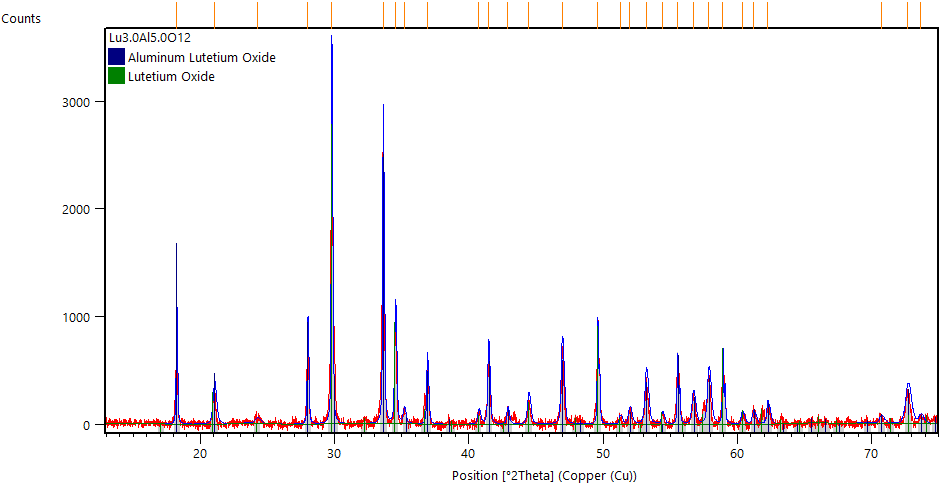
\includegraphics[width=\textwidth]{Anexos/x=0.png}%
		\caption{Análisis del patrón de difracción de rayos X de la muestra
		\ce{Lu_{3.0}Al_{5.0}O12}} \label{fig:XpertX0}
	\end{figure}

	\begin{figure}[h]
		\centering%
		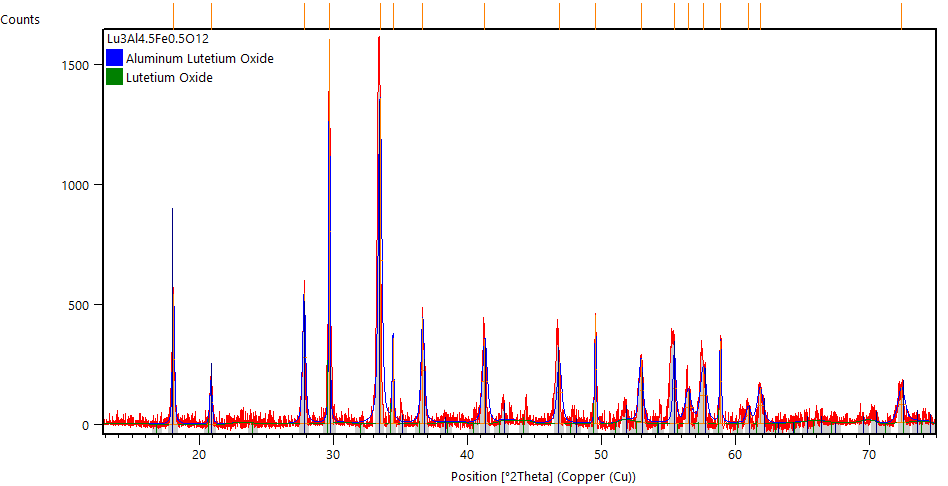
\includegraphics[width=\textwidth]{Anexos/x=05.png}%
		\caption{Análisis del patrón de difracción de rayos X de la muestra
		\ce{Lu_{3.0}Al_{4.5}Fe_{0.5}O12}} \label{fig:XpertX05}
	\end{figure}

	\begin{figure}[h]
		\centering%
		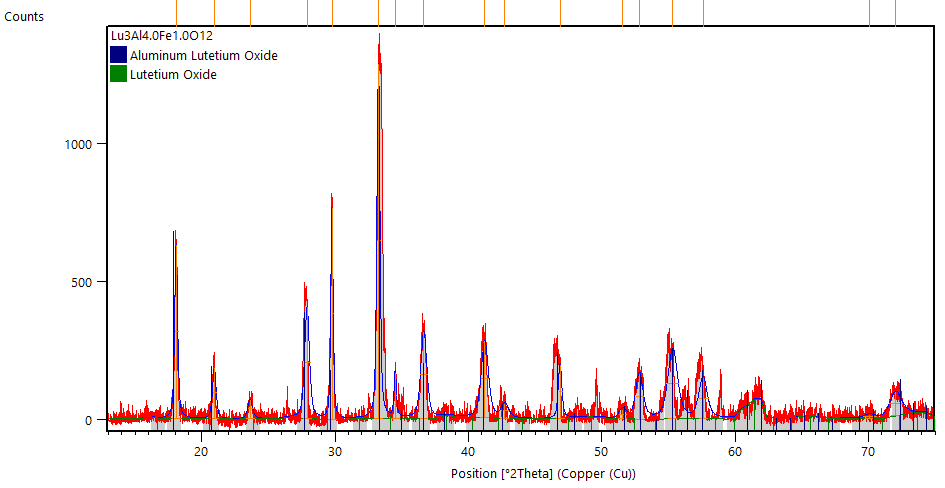
\includegraphics[width=\textwidth]{Anexos/x=10.png}%
		\caption{Análisis del patrón de difracción de rayos X de la muestra
		\ce{Lu_{3.0}Al_{4.0}Fe_{1.0}O12}}
		\label{fig:XpertX10}
	\end{figure}

	\begin{figure}[h]
		\centering%
		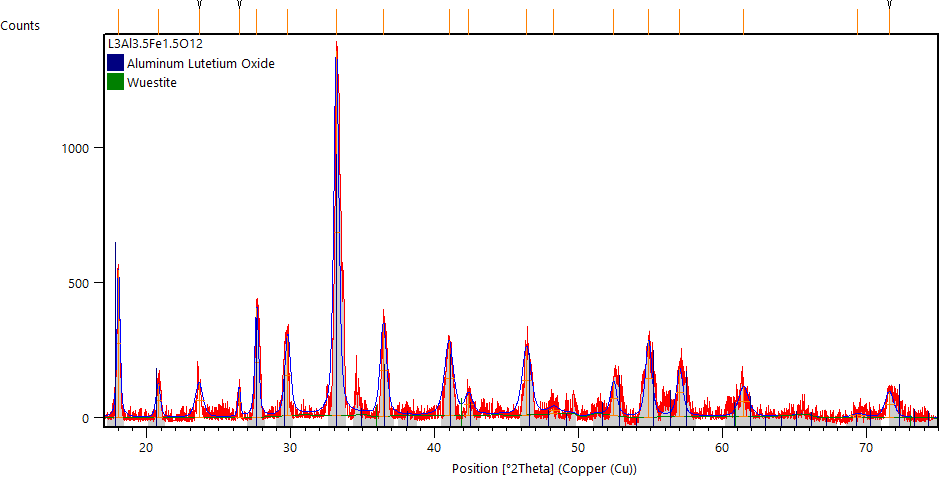
\includegraphics[width=\textwidth]{Anexos/x=15.png}%
		\caption{Análisis del patrón de difracción de rayos X de la muestra
		\ce{Lu_{3.0}Al_{3.5}Fe_{1.5}O12}} \label{fig:XpertX15}
	\end{figure}

	\begin{figure}[h]
		\centering%
		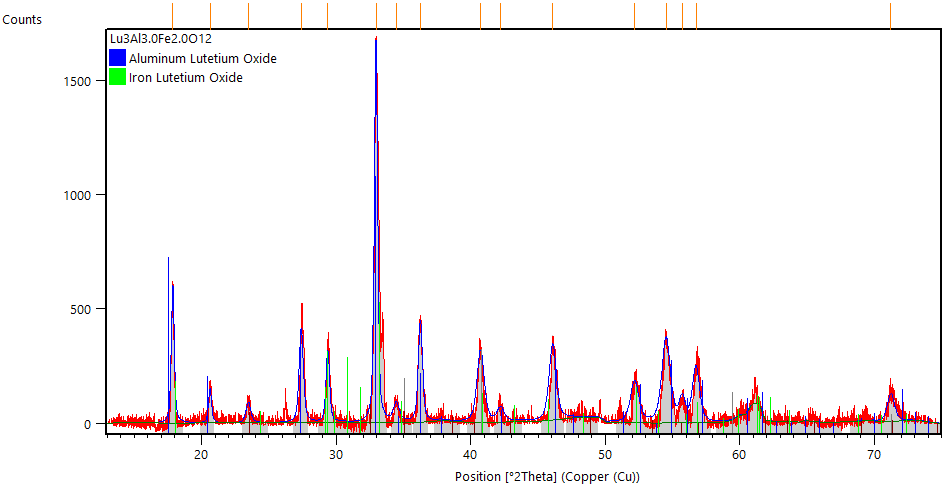
\includegraphics[width=\textwidth]{Anexos/x=20.png}%
		\caption{Análisis del patrón de difracción de rayos X de la muestra
		\ce{Lu_{3.0}Al_{3.0}Fe_{2.0}O12}} \label{fig:XpertX20}
	\end{figure}

	\begin{figure}[h]
		\centering%
		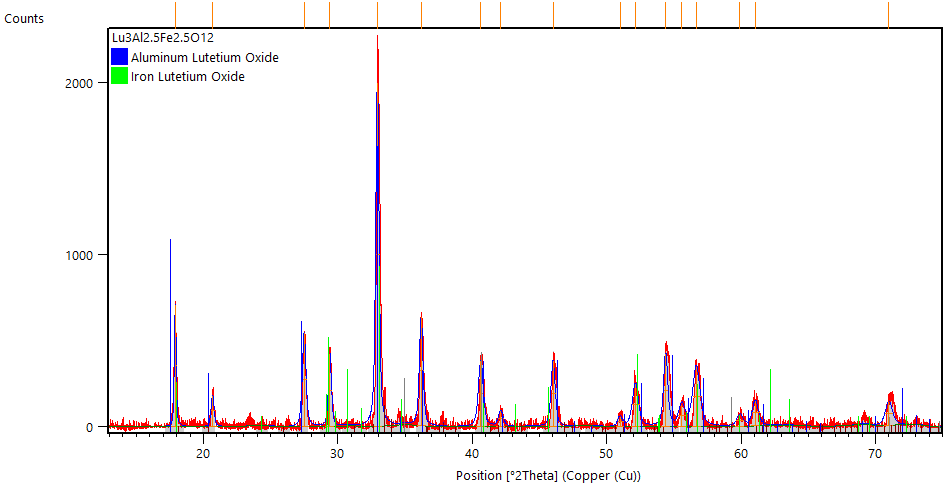
\includegraphics[width=\textwidth]{Anexos/x=25.png}%
		\caption{Análisis del patrón de difracción de rayos X de la muestra
		\ce{Lu_{3.0}Al_{2.5}Fe_{2.5}O12}}  \label{fig:XpertX25}
	\end{figure}

	\begin{figure}[h]
		\centering%
		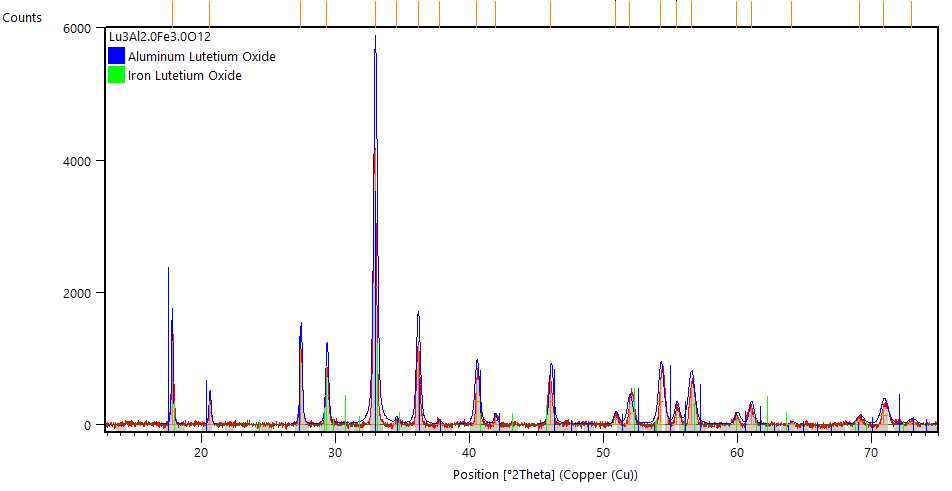
\includegraphics[width=\textwidth]{Anexos/x=30.png}%
		\caption{Análisis del patrón de difracción de rayos X de la muestra
		\ce{Lu_{3.0}Al_{2.0}Fe_{3.0}O12}} \label{fig:XpertX30}
	\end{figure}

	\begin{figure}[h]
		\centering%
		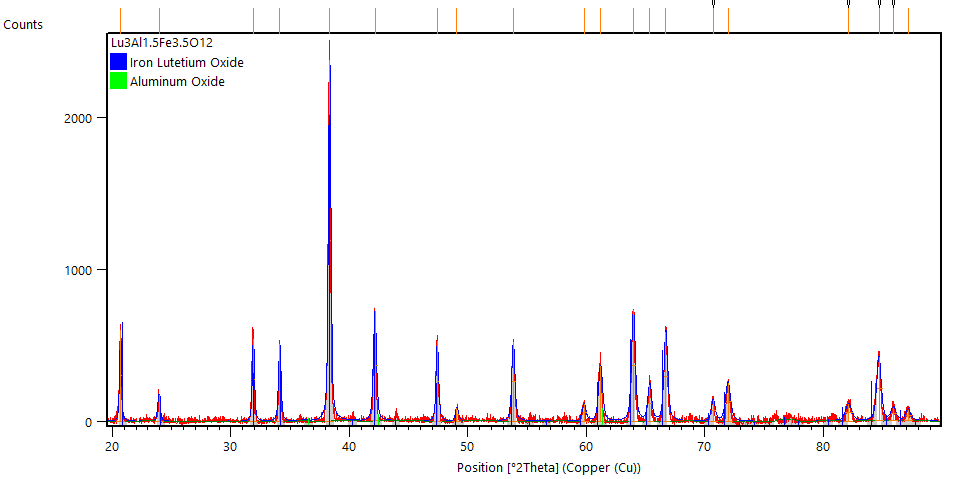
\includegraphics[width=\textwidth]{Anexos/x=35}%
		\caption{Análisis del patrón de difracción de rayos X de la muestra
		\ce{Lu_{3.0}Al_{1.5}Fe_{3.5}O12}} \label{fig:XpertX35}
	\end{figure}

	\begin{figure}[h]
		\centering%
		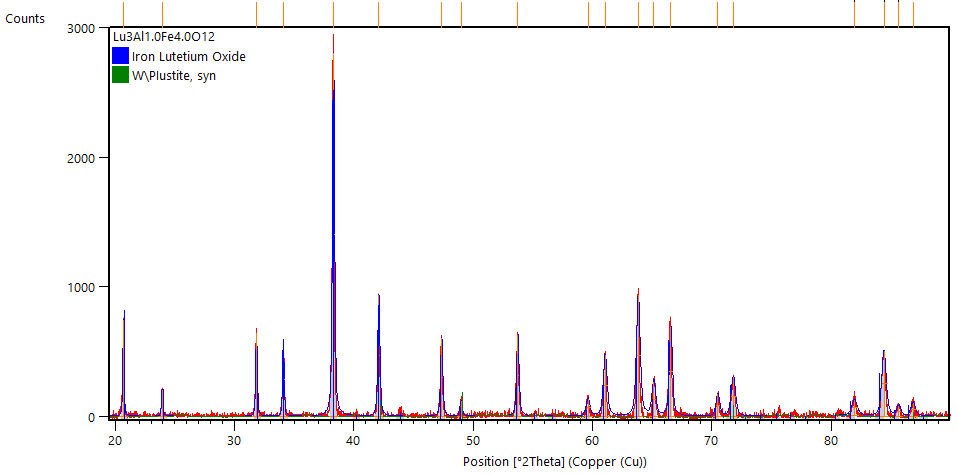
\includegraphics[width=\textwidth]{Anexos/x=40.png}%
		\caption{Análisis del patrón de difracción de rayos X de la muestra
		\ce{Lu_{3.0}Al_{1.0}Fe_{4.0}O12}} \label{fig:XpertX40}
	\end{figure}

	\begin{figure}[t!]
		\centering%
		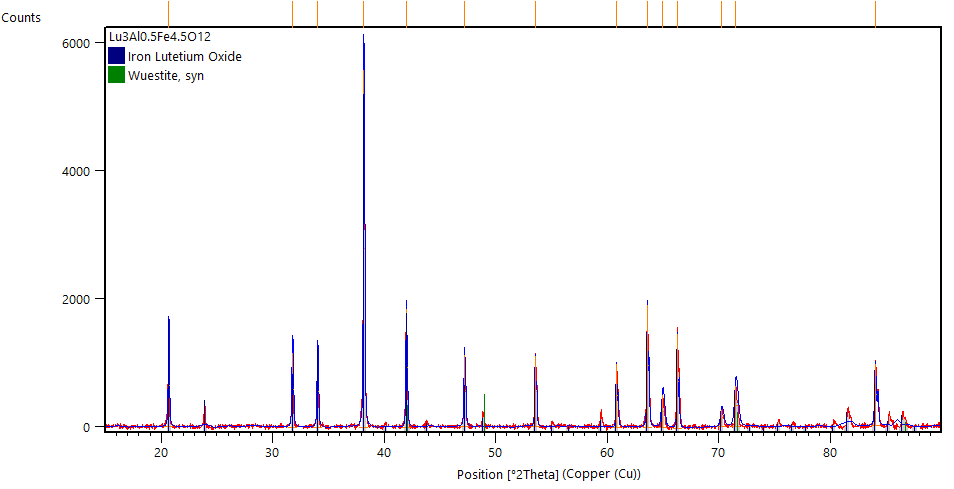
\includegraphics[width=\textwidth]{Anexos/x=45.png}%
		\caption{Análisis del patrón de difracción de rayos X de la muestra
		\ce{Lu_{3.0}Al_{0.5}Fe_{4.5}O12}} \label{fig:XpertX45}
	\end{figure}

	\chapter{Refinamiento Rietveld}\label{AnexoB}

	\begin{figure}[h]
		\centering%
		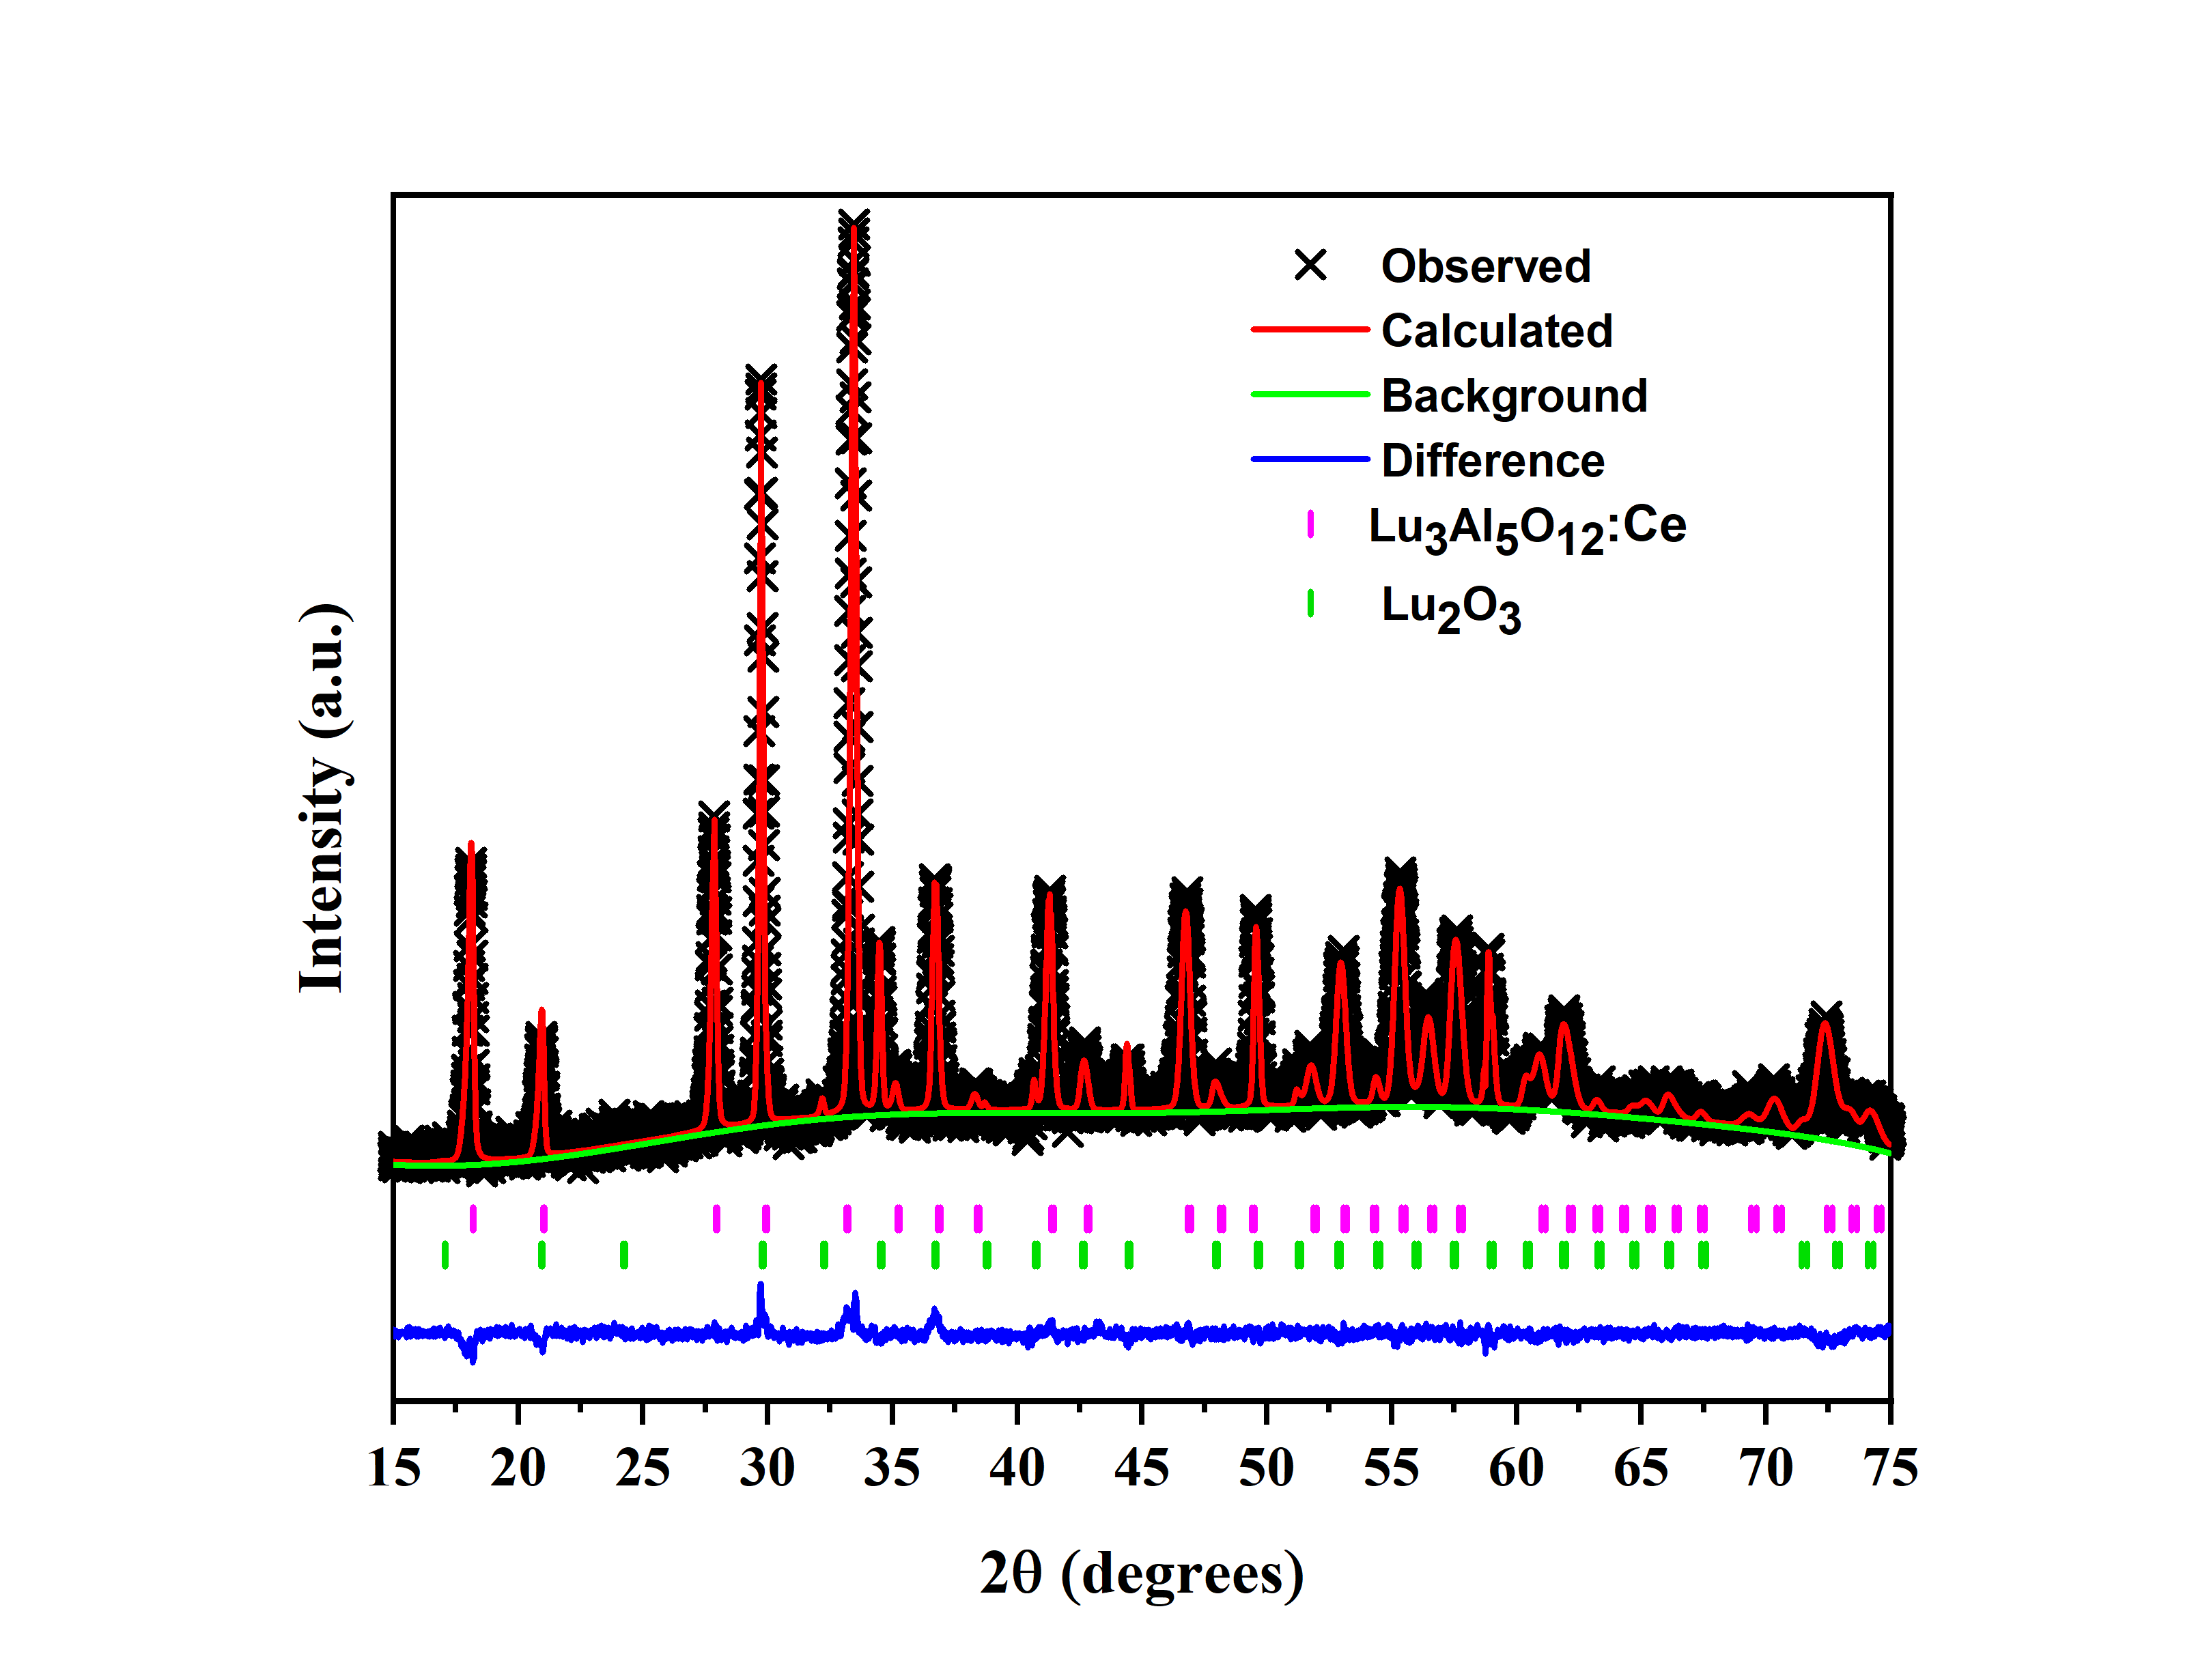
\includegraphics[width=12cm]{Anexos/x00.png}%
		\caption{Resultados de refinamiento Rietveld de a \ce{Lu_{3.0}Al_{5.0}O12}}
		\label{fig:Refi00}
	\end{figure}

	\begin{figure}[h]
		\centering%
		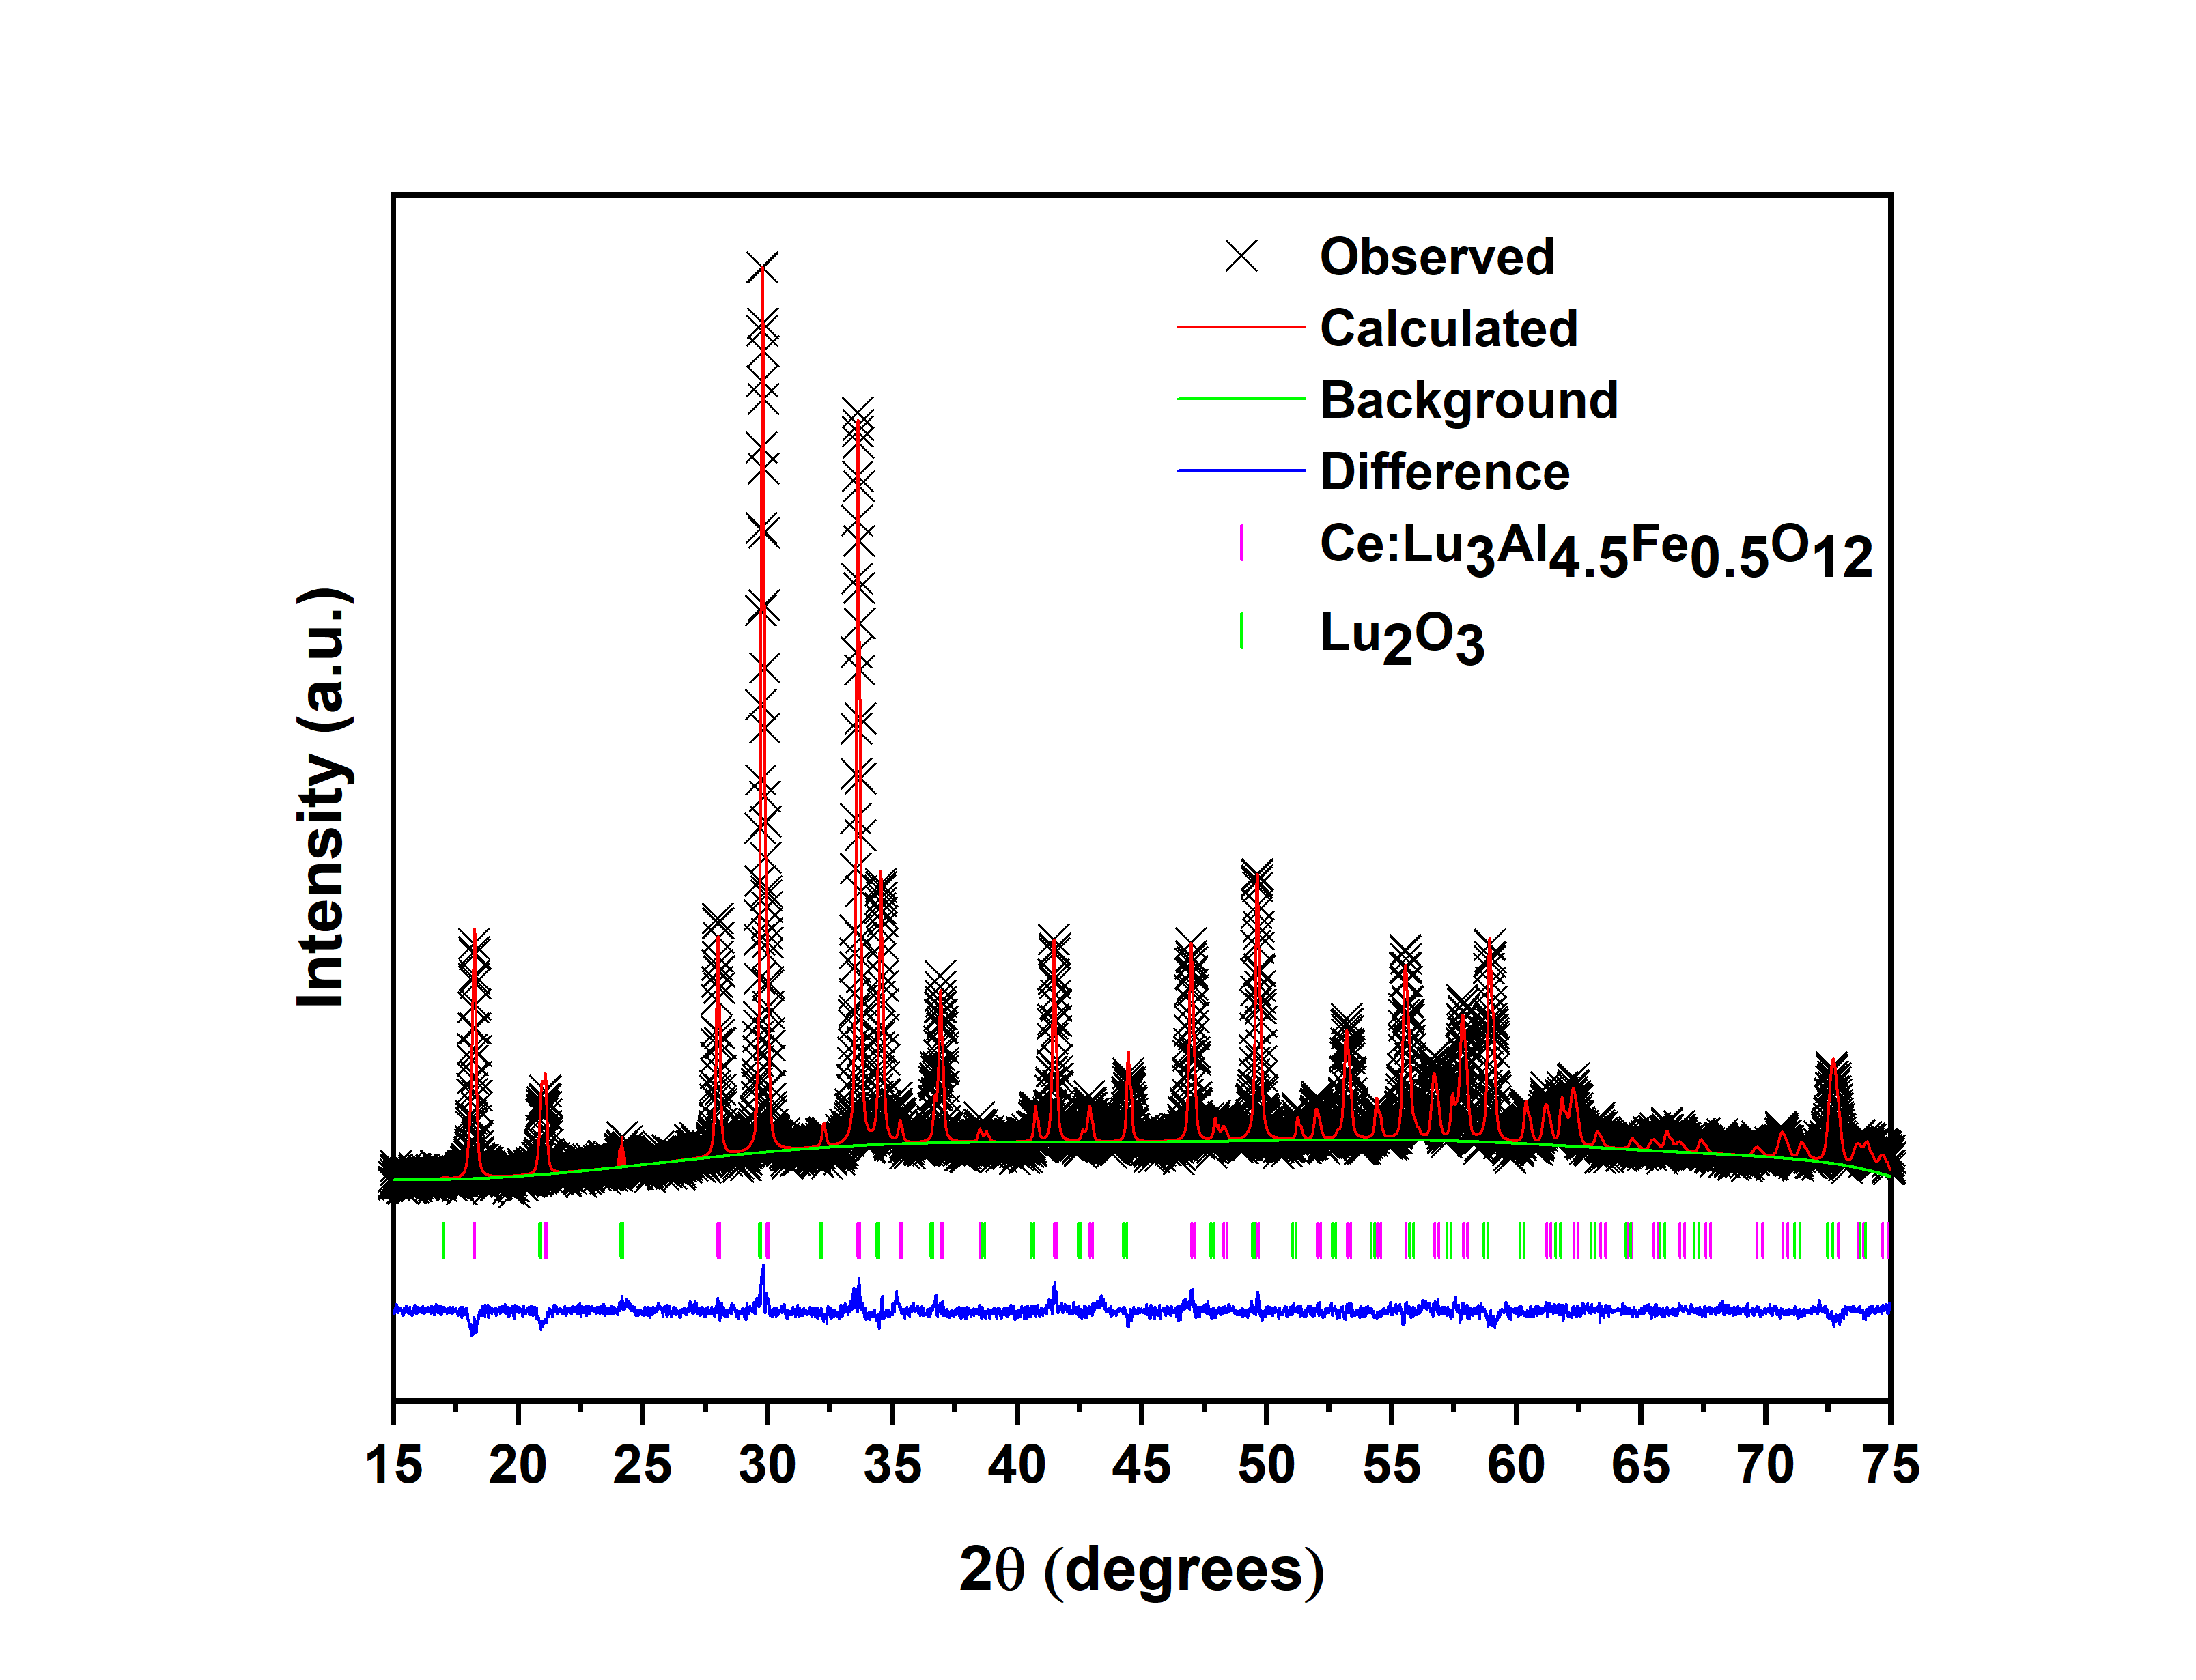
\includegraphics[width=11cm]{Anexos/x05.png}%
		\caption{Resultados de refinamiento Rietveld de
		\ce{Lu_{3.0}Al_{4.5}Fe_{0.5}O12}} \label{fig:refi05}
	\end{figure}

	\begin{figure}[h]
		\centering%
		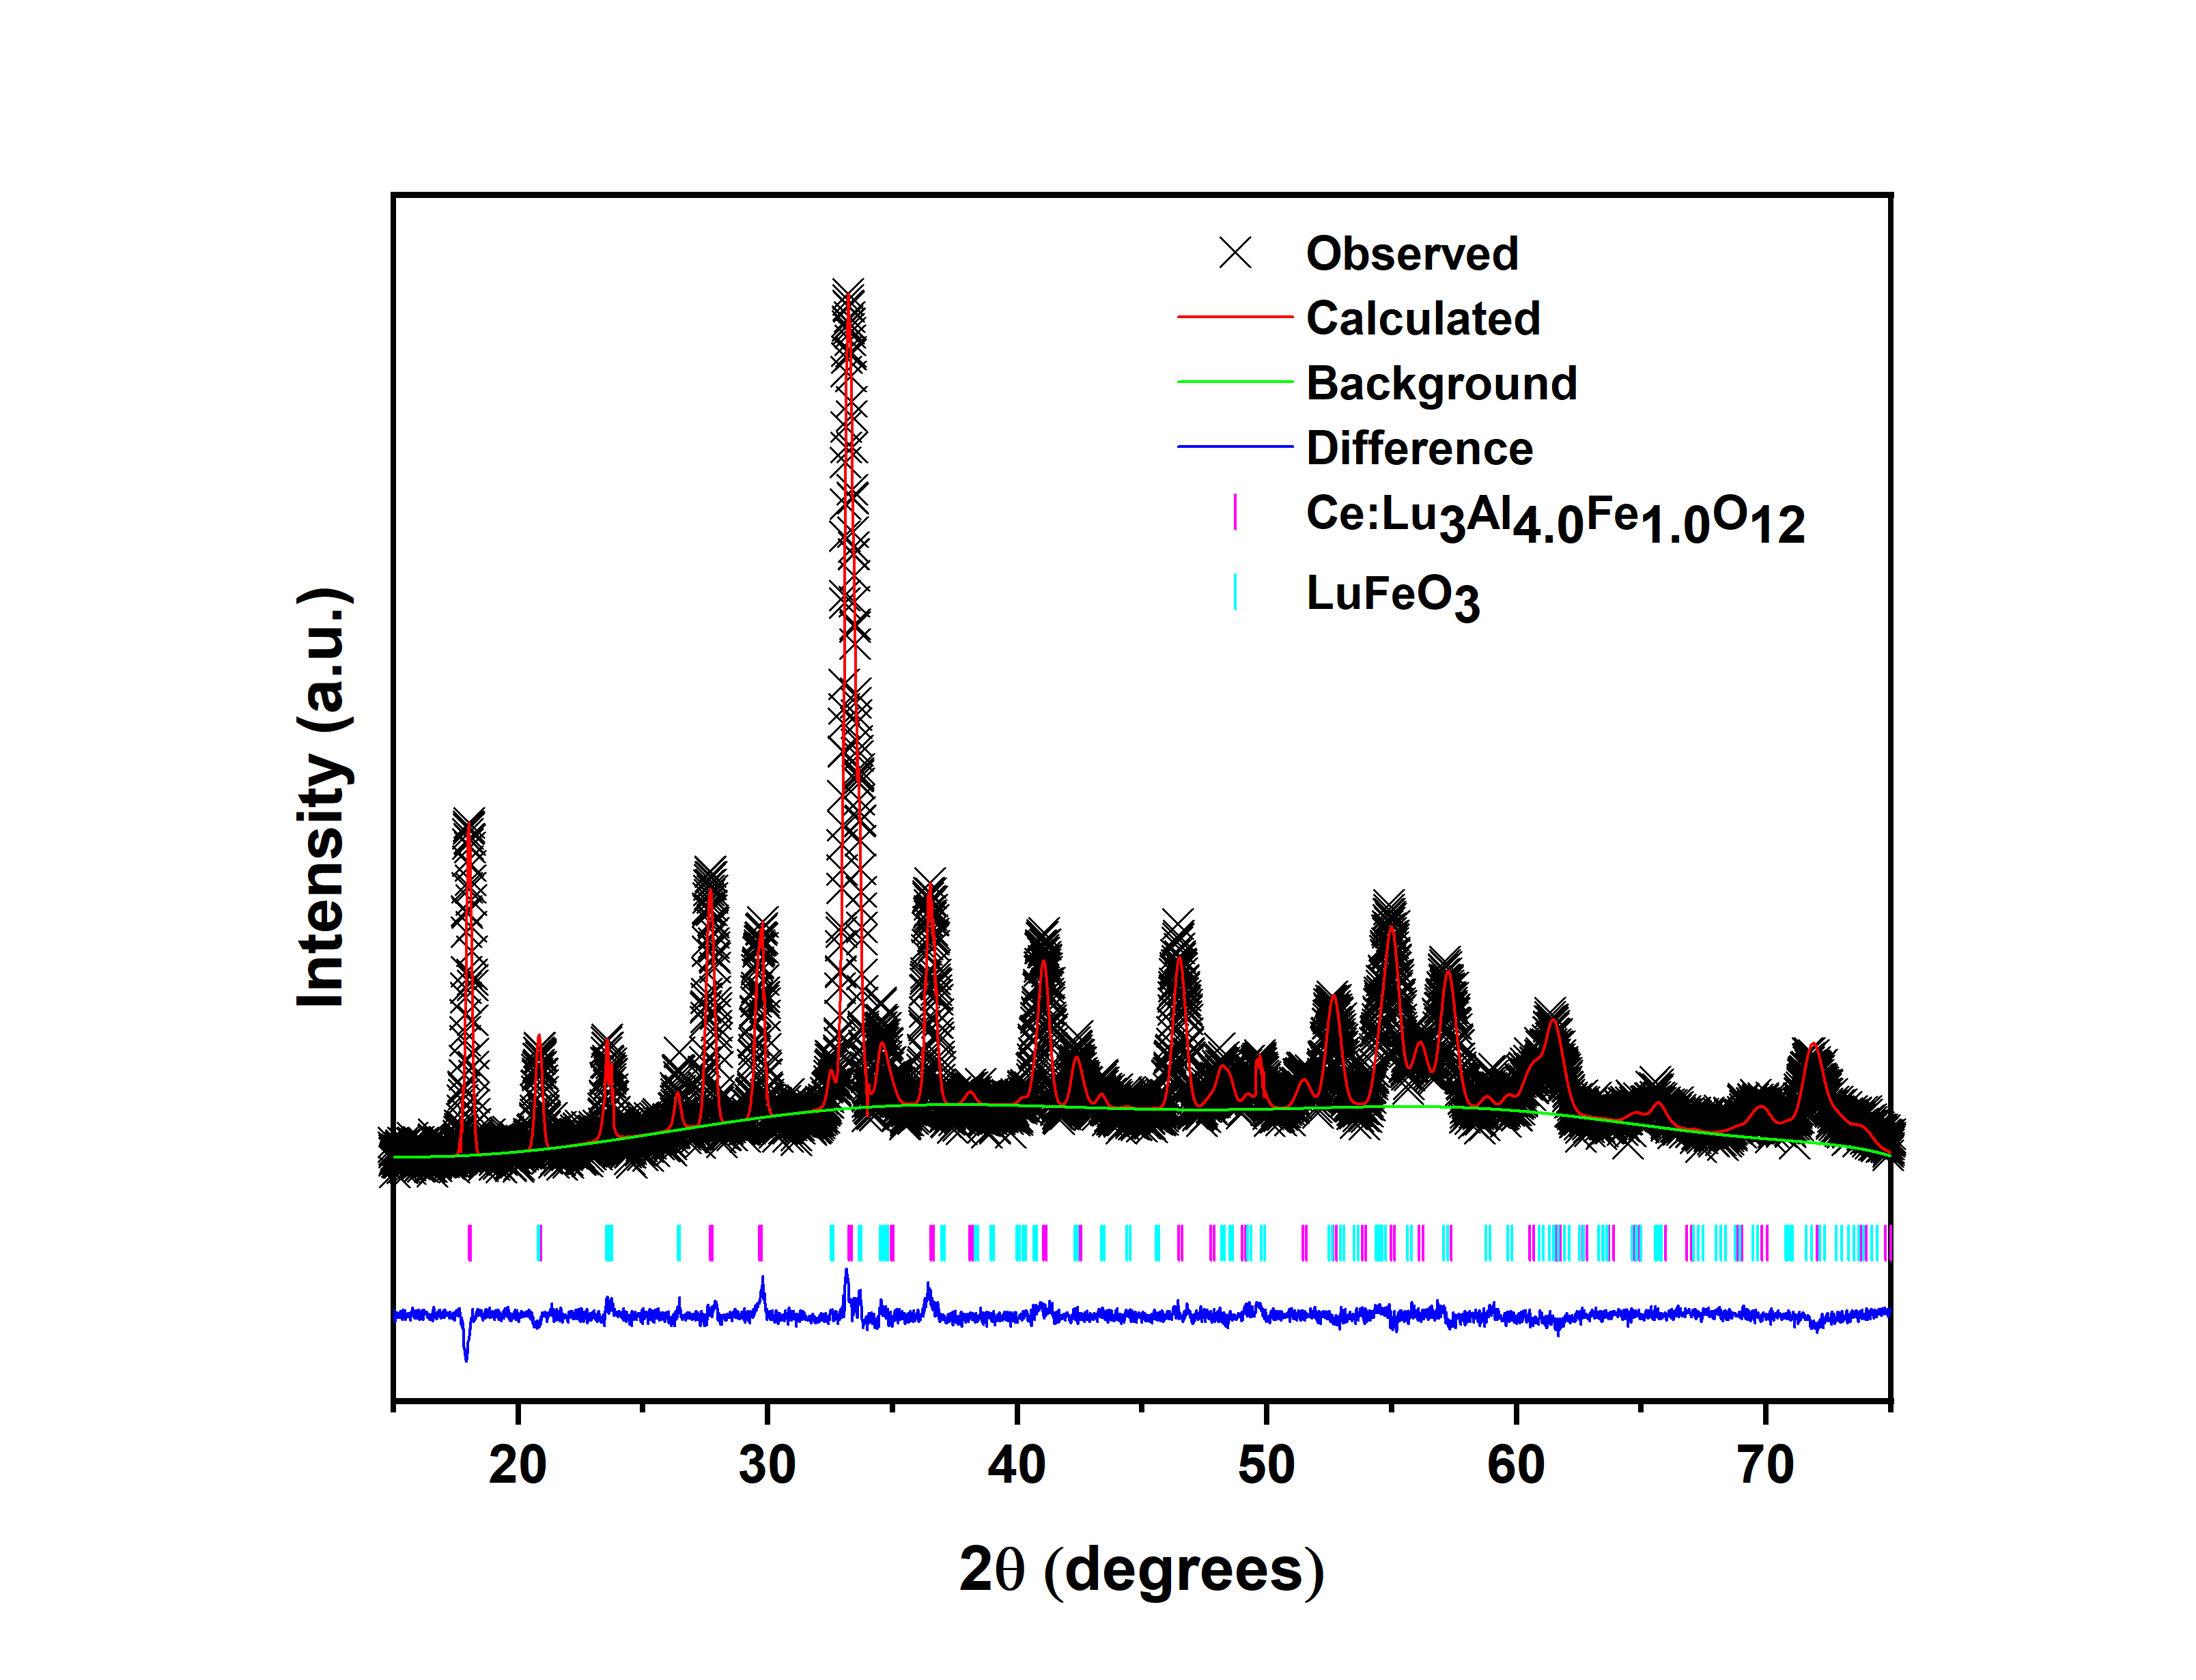
\includegraphics[width=11cm]{Anexos/x10.png}%
		\caption{Resultados de refinamiento Rietveld de
		\ce{Lu_{3.0}Al_{4.0}Fe_{1.0}O12}}\label{fig:refi10}
	\end{figure}

	\begin{figure}[h]
		\centering%
		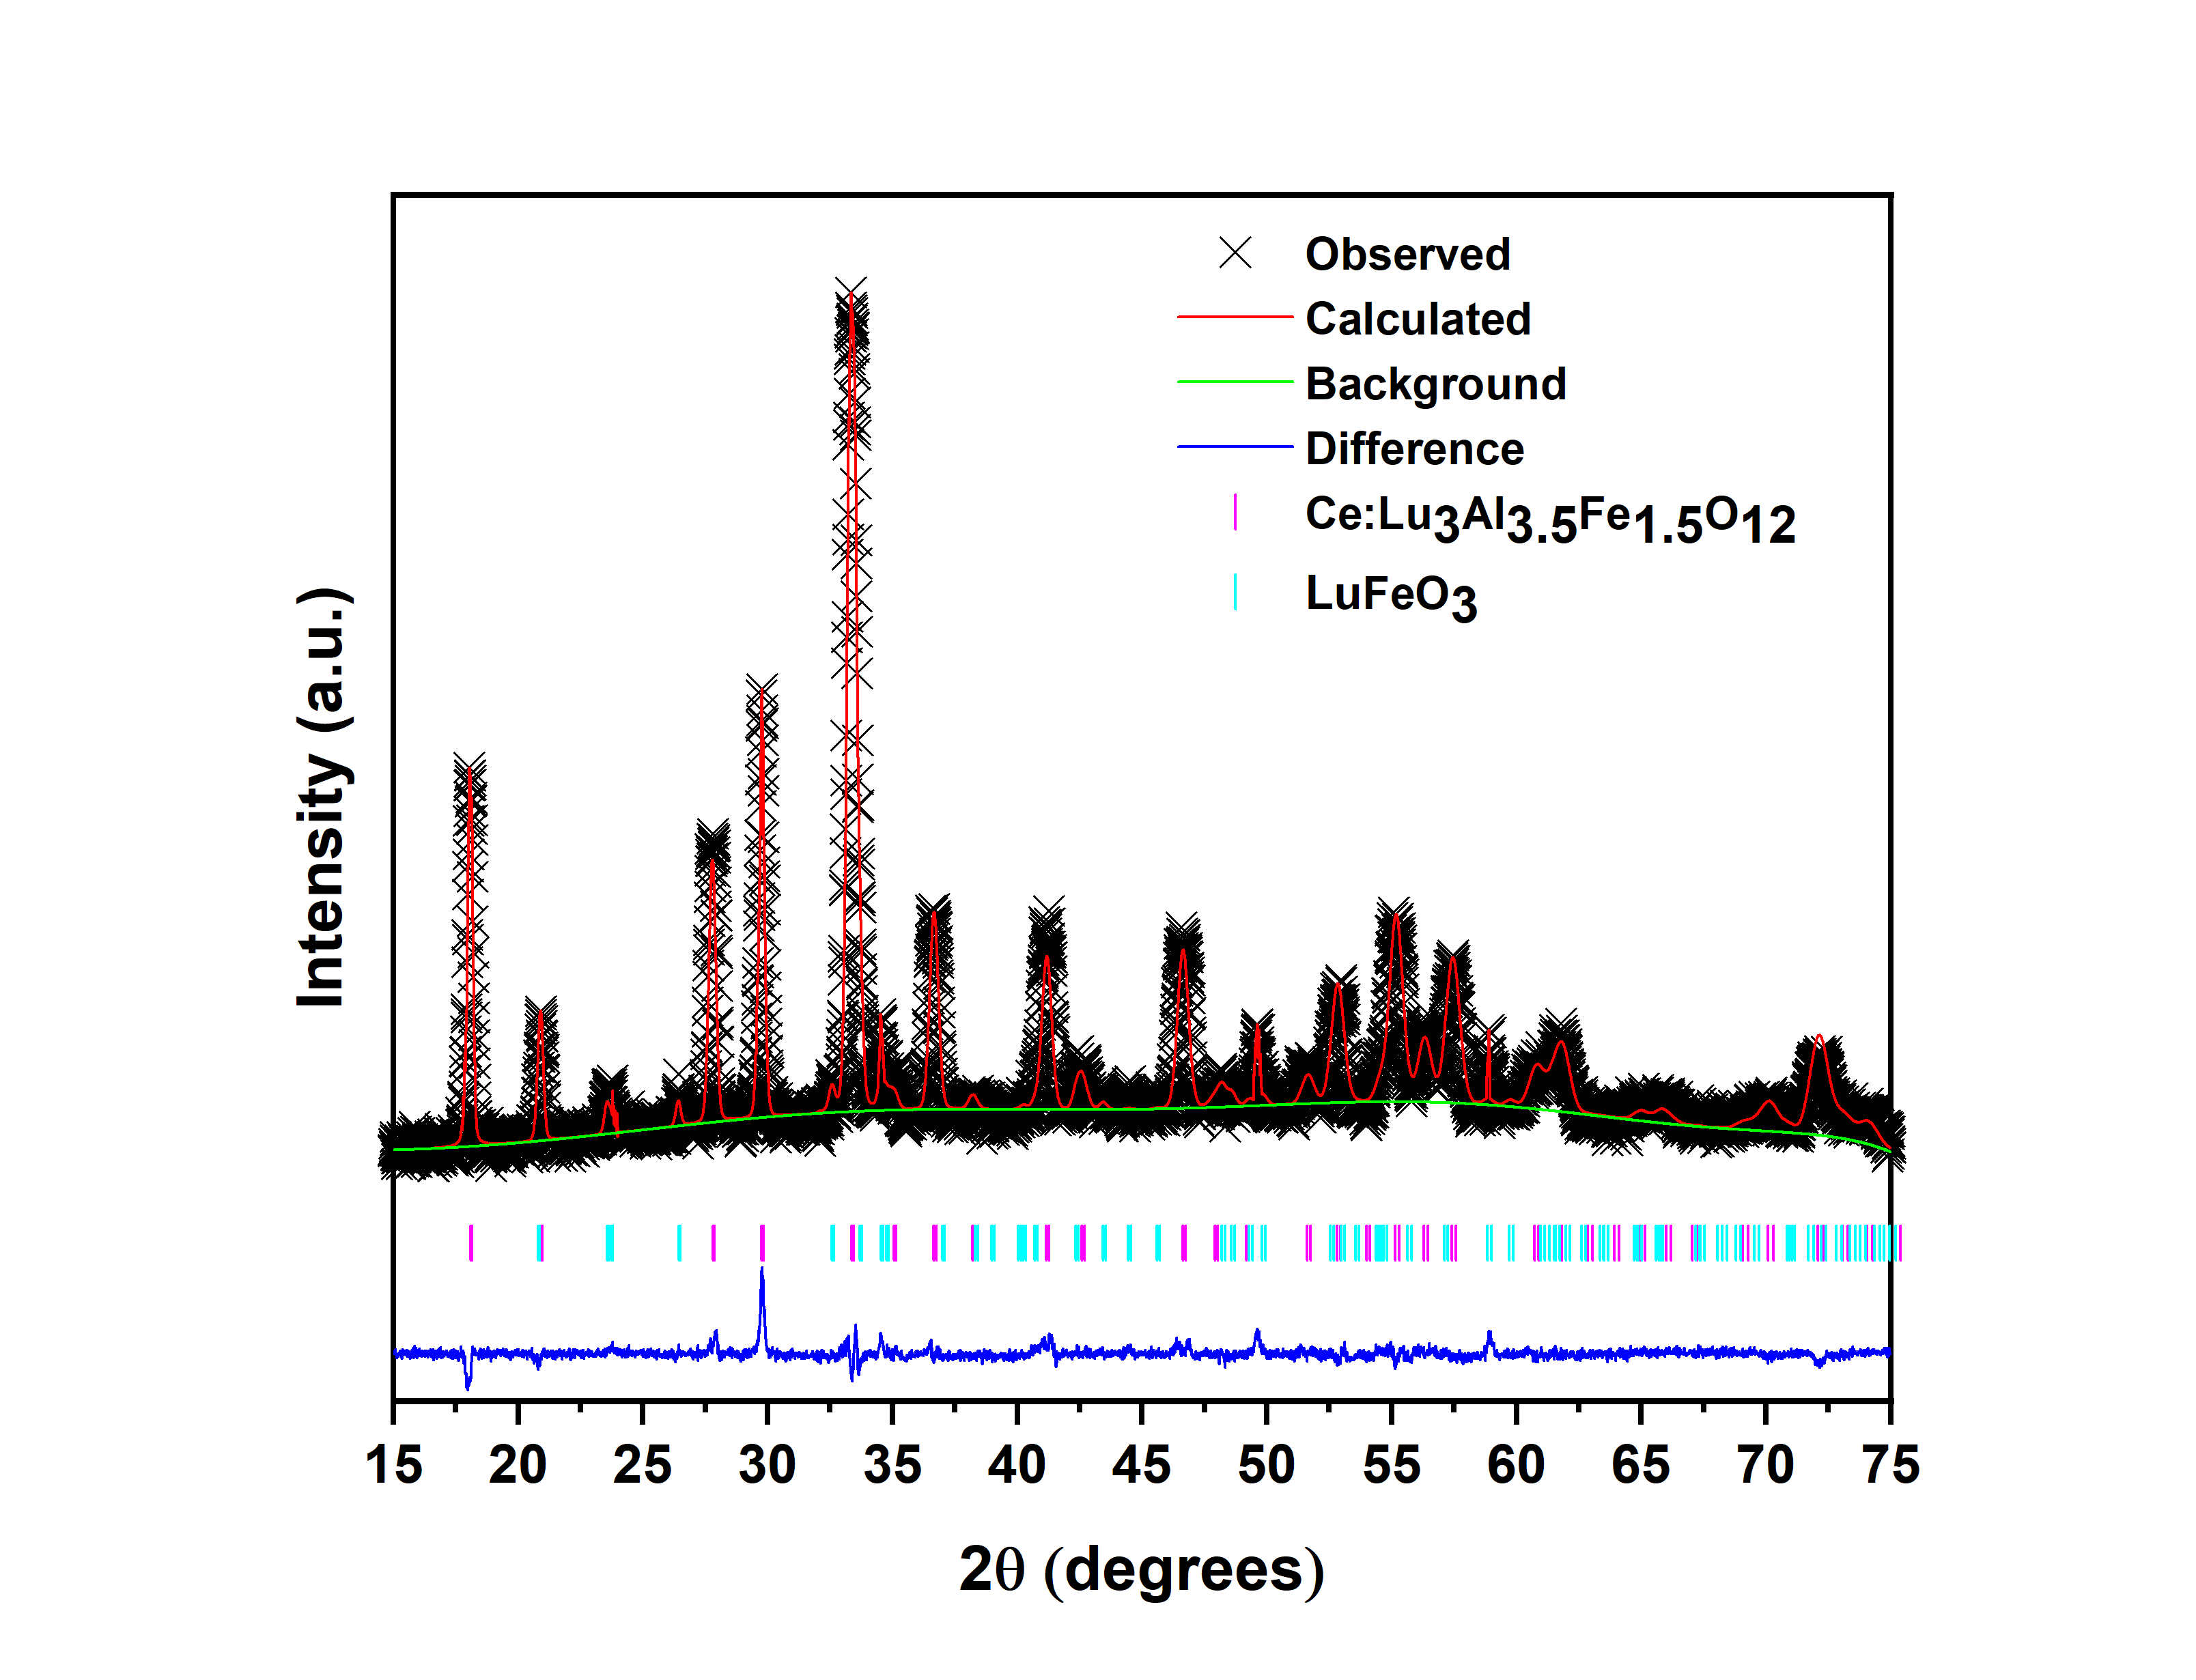
\includegraphics[width=11cm]{Anexos/x15.png}%
		\caption{Resultados de refinamiento Rietveld de
		\ce{Lu_{3.0}Al_{3.5}Fe_{1.5}O12}}\label{fig:refi15}
	\end{figure}

	\begin{figure}[h]
		\centering%
		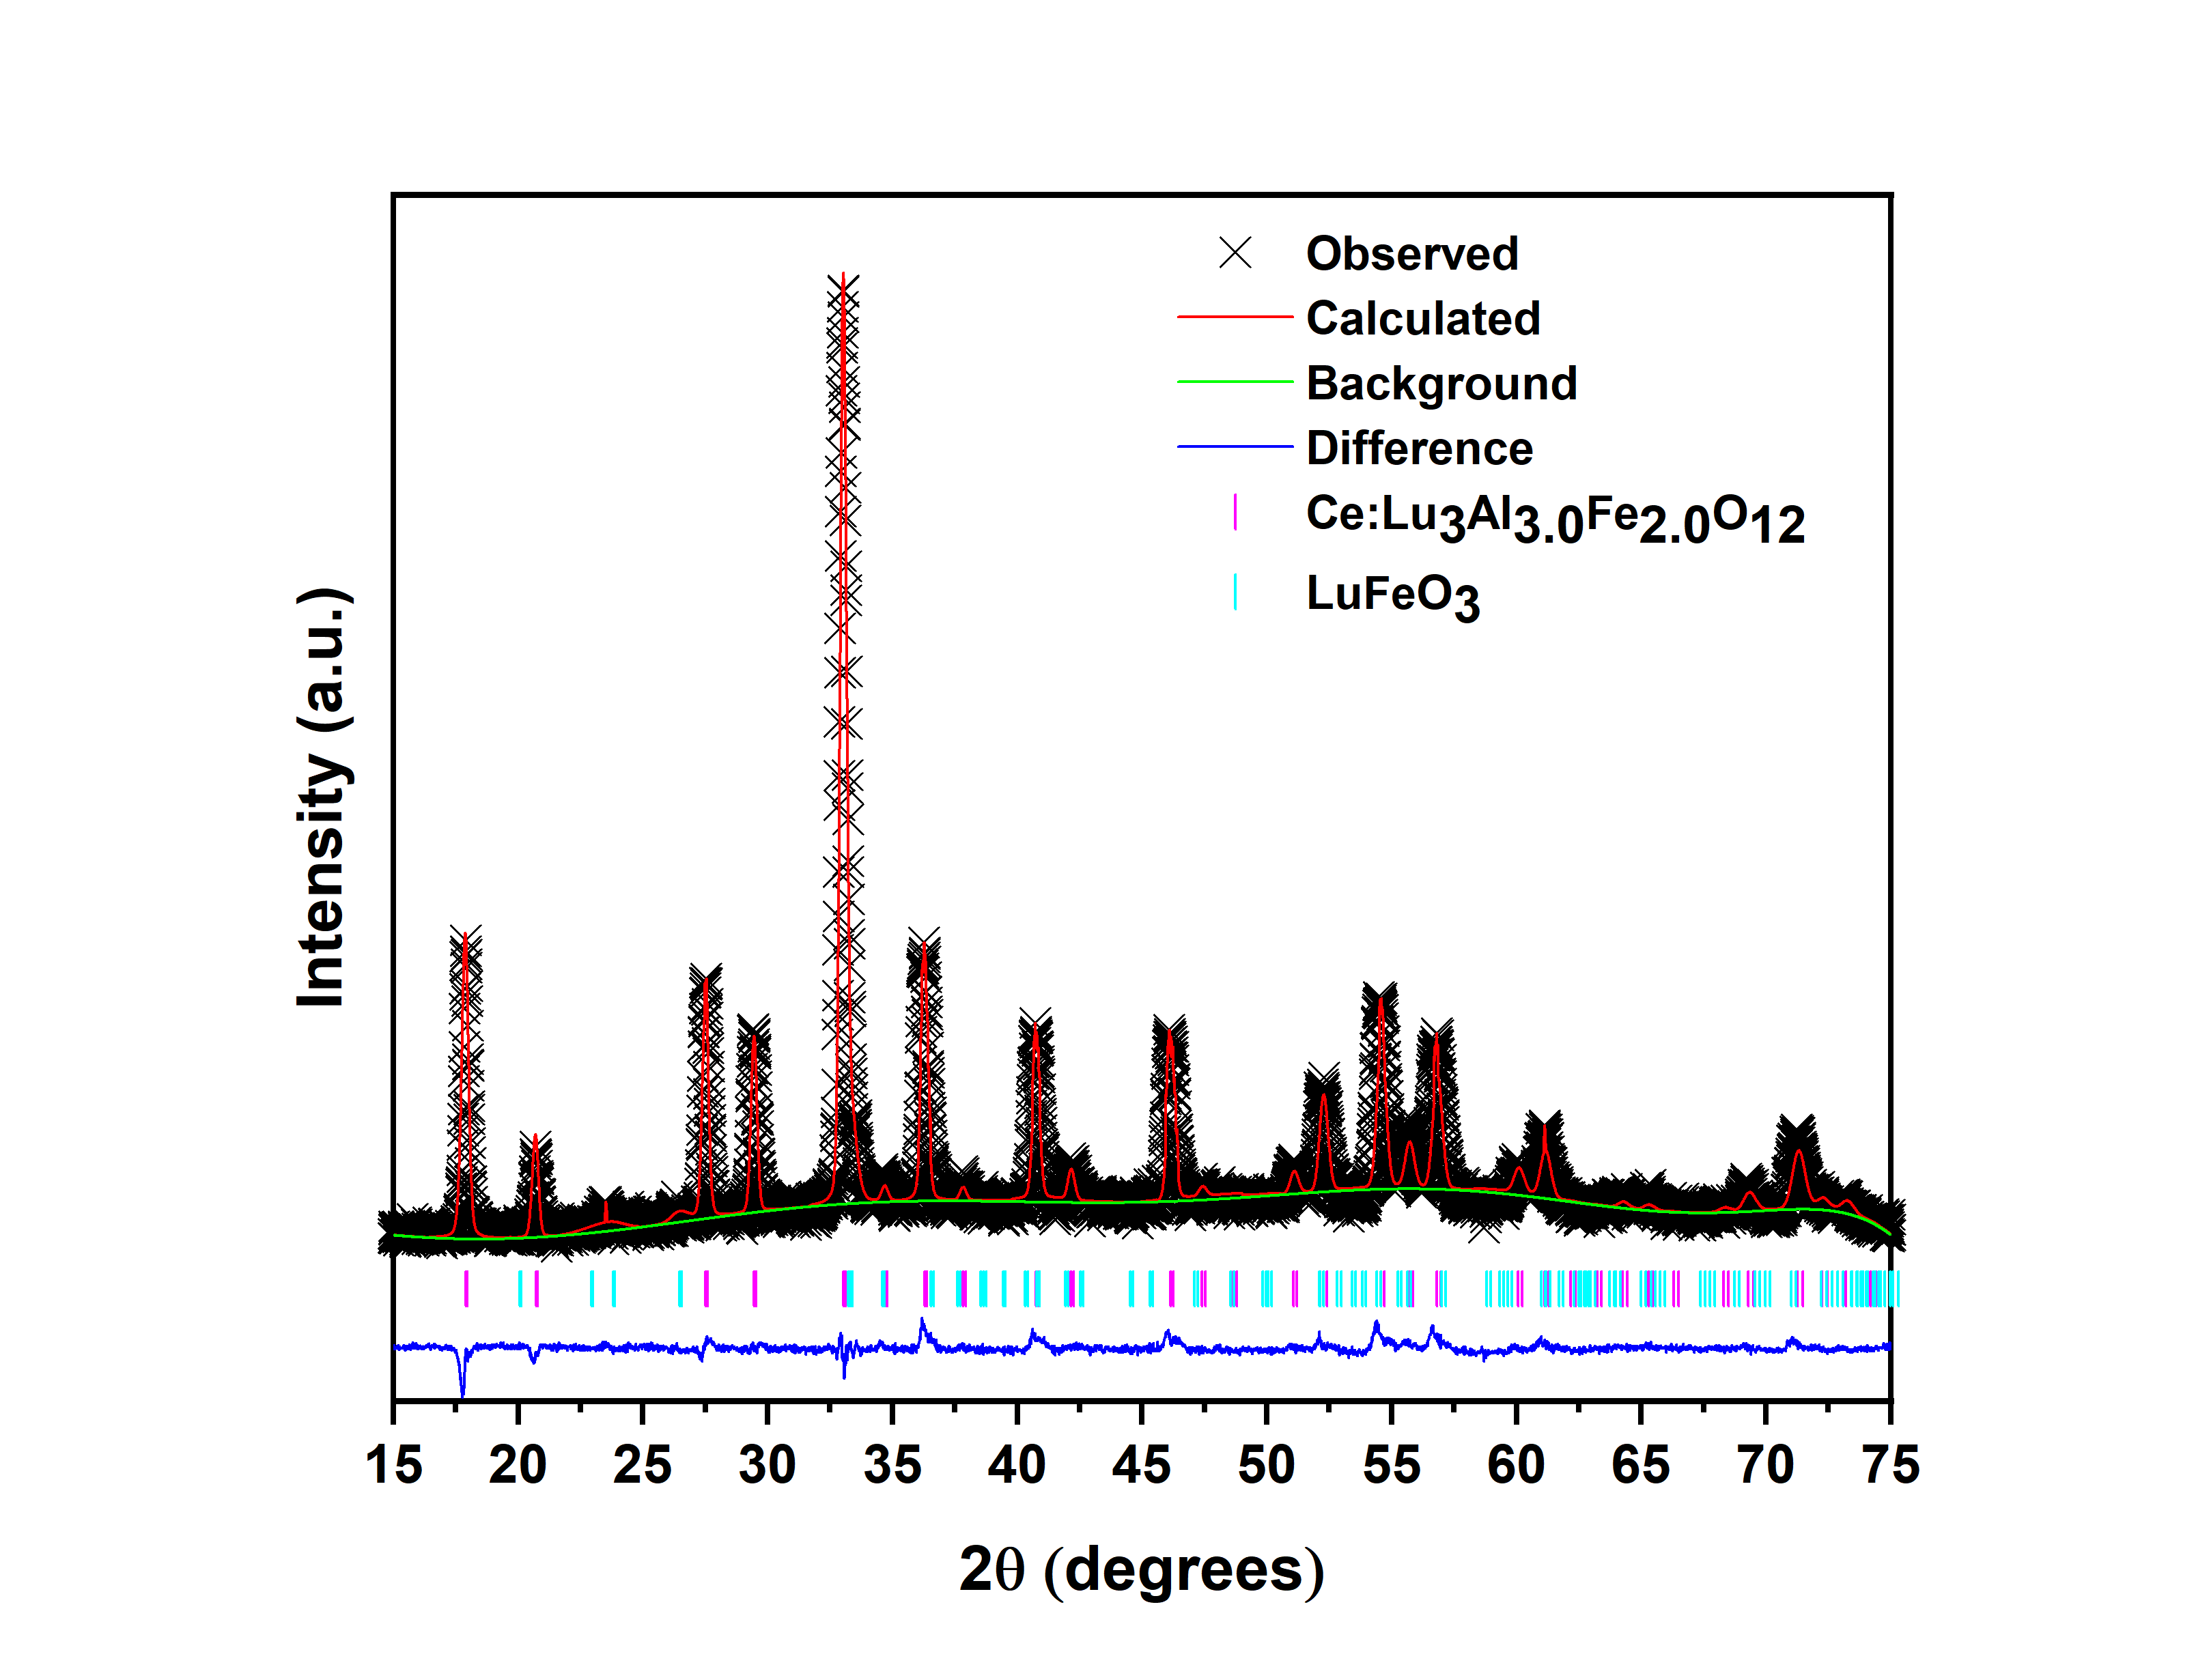
\includegraphics[width=11cm]{Anexos/x20.png}%
		\caption{Resultados de refinamiento Rietveld de
		\ce{Lu_{3.0}Al_{3.0}Fe_{2.0}O12}}\label{fig:refi20}
	\end{figure}

	\begin{figure}[h]
		\centering%
		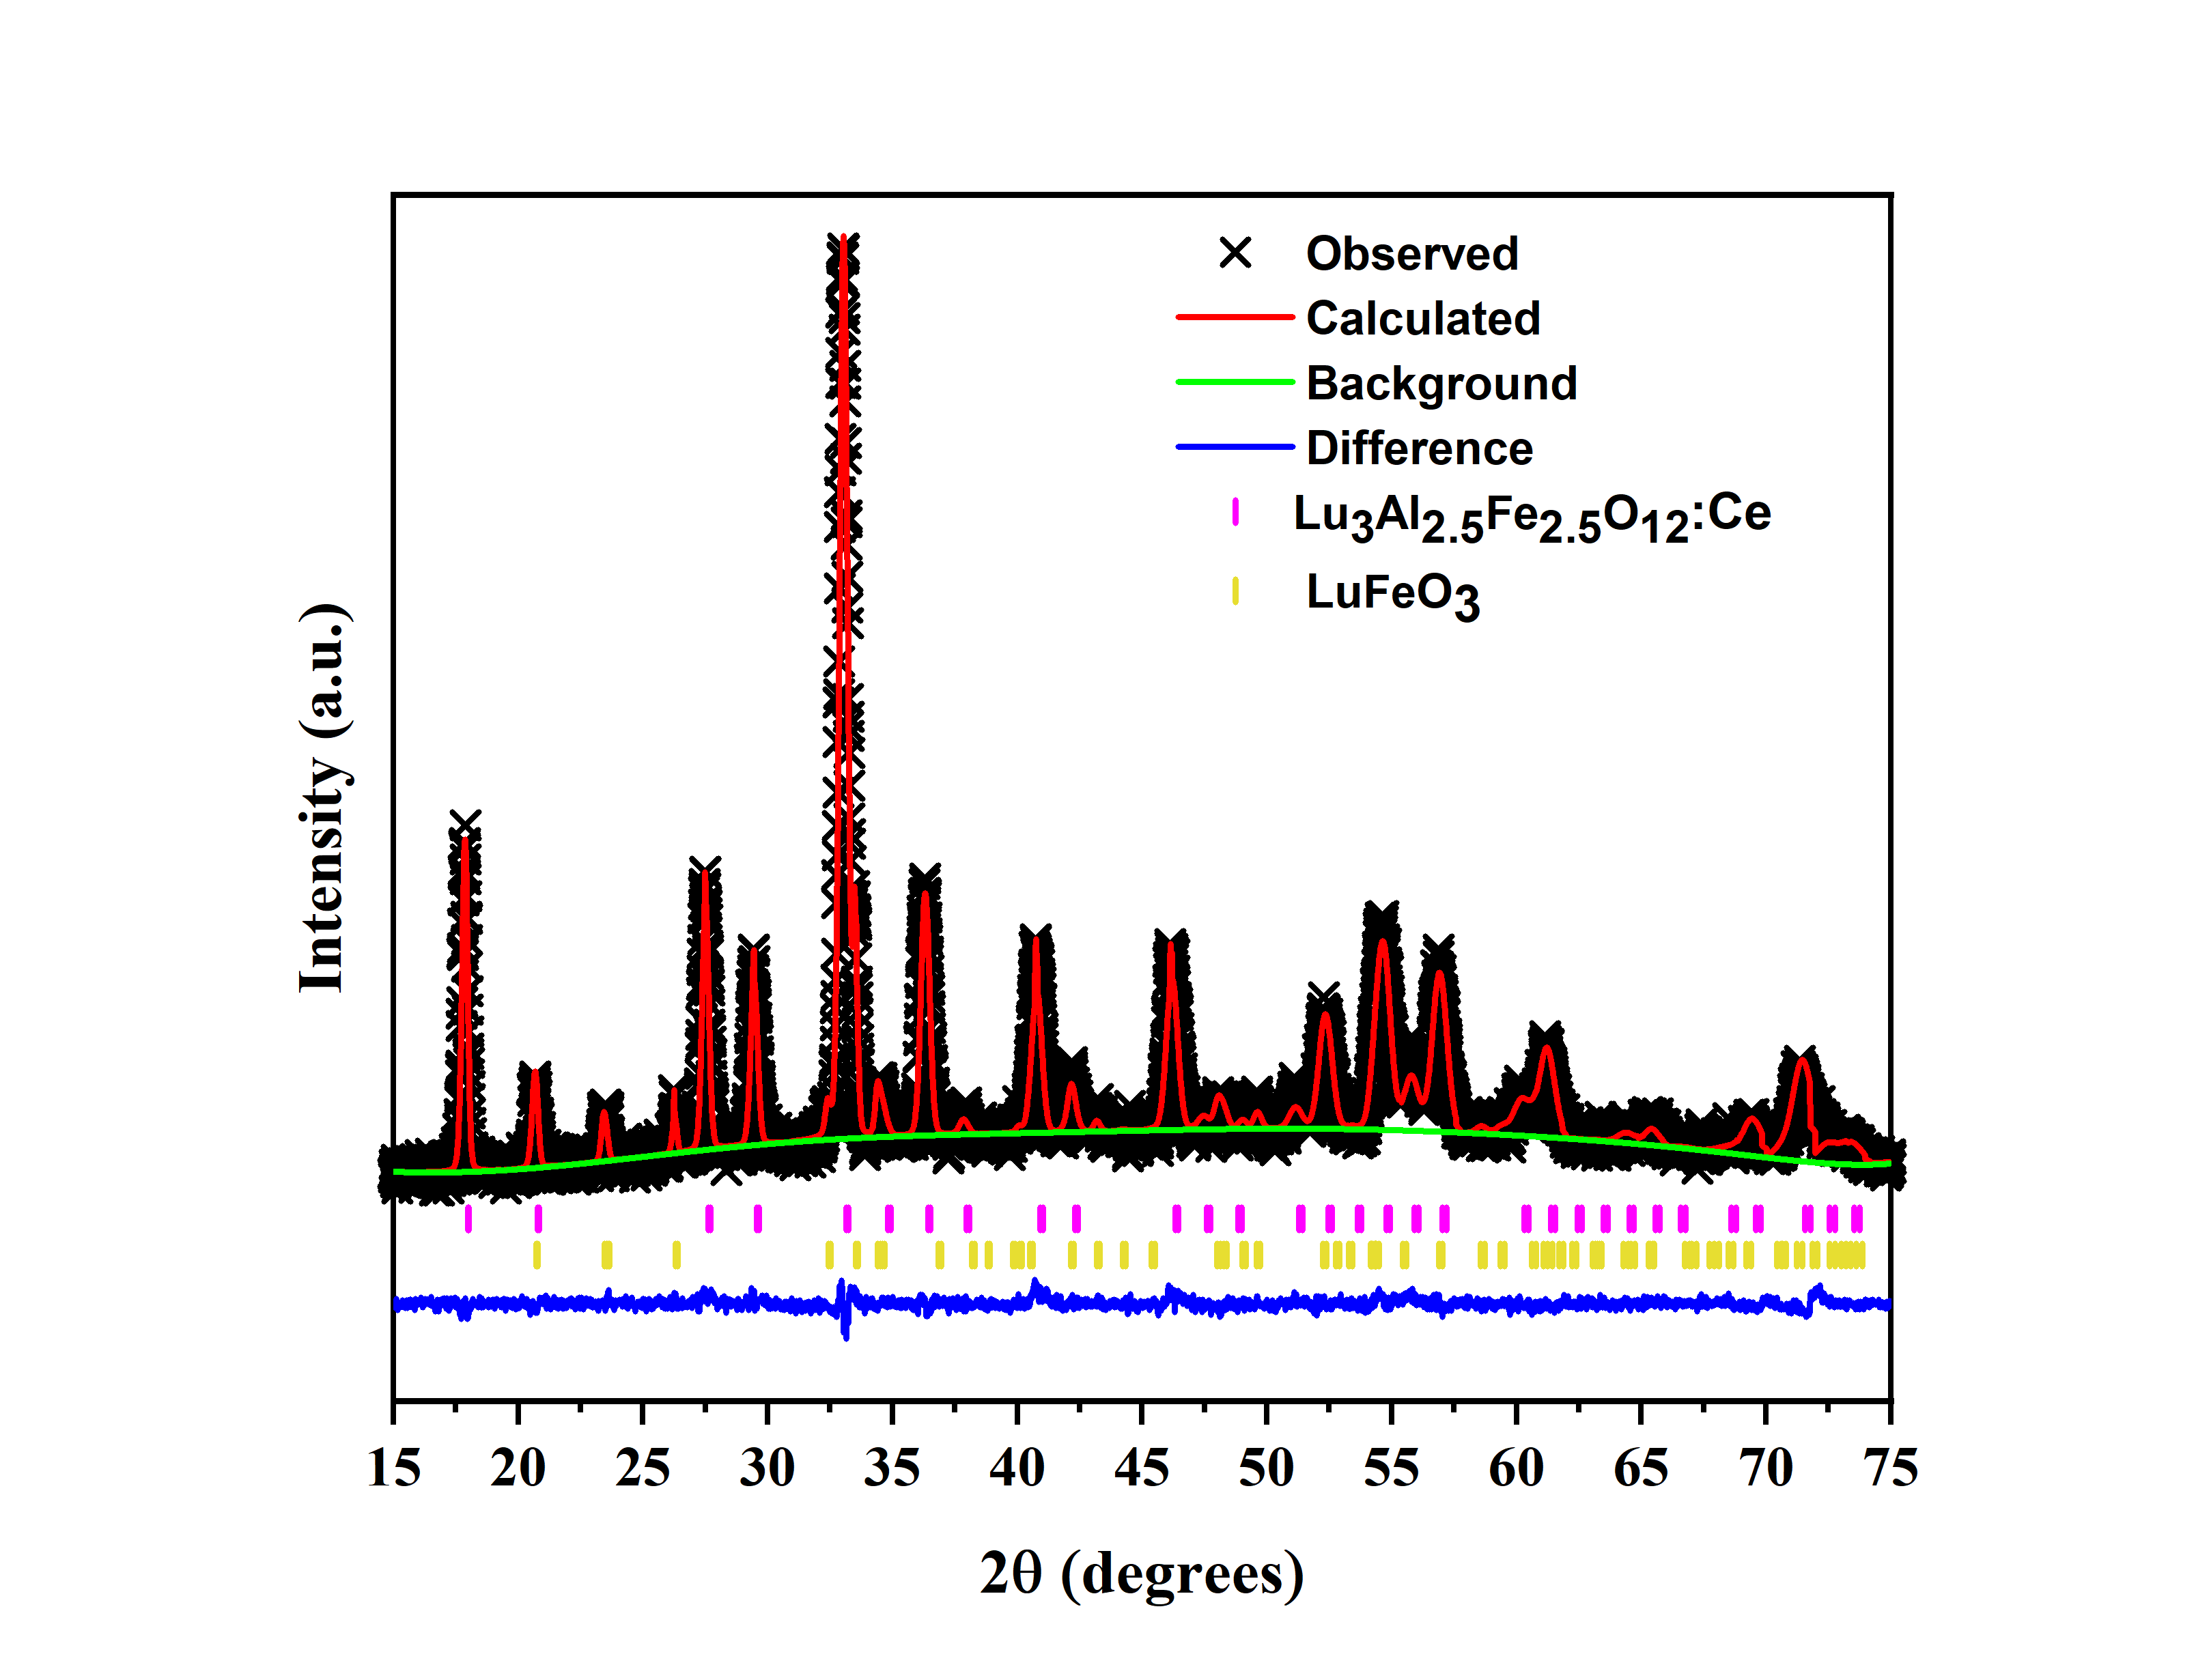
\includegraphics[width=11cm]{Anexos/x25.png}%
		\caption{Resultados de refinamiento Rietveld de
		\ce{Lu_{3.0}Al_{2.5}Fe_{2.5}O12}}\label{fig:refi25}
	\end{figure}

	\begin{figure}[h]
		\centering%
		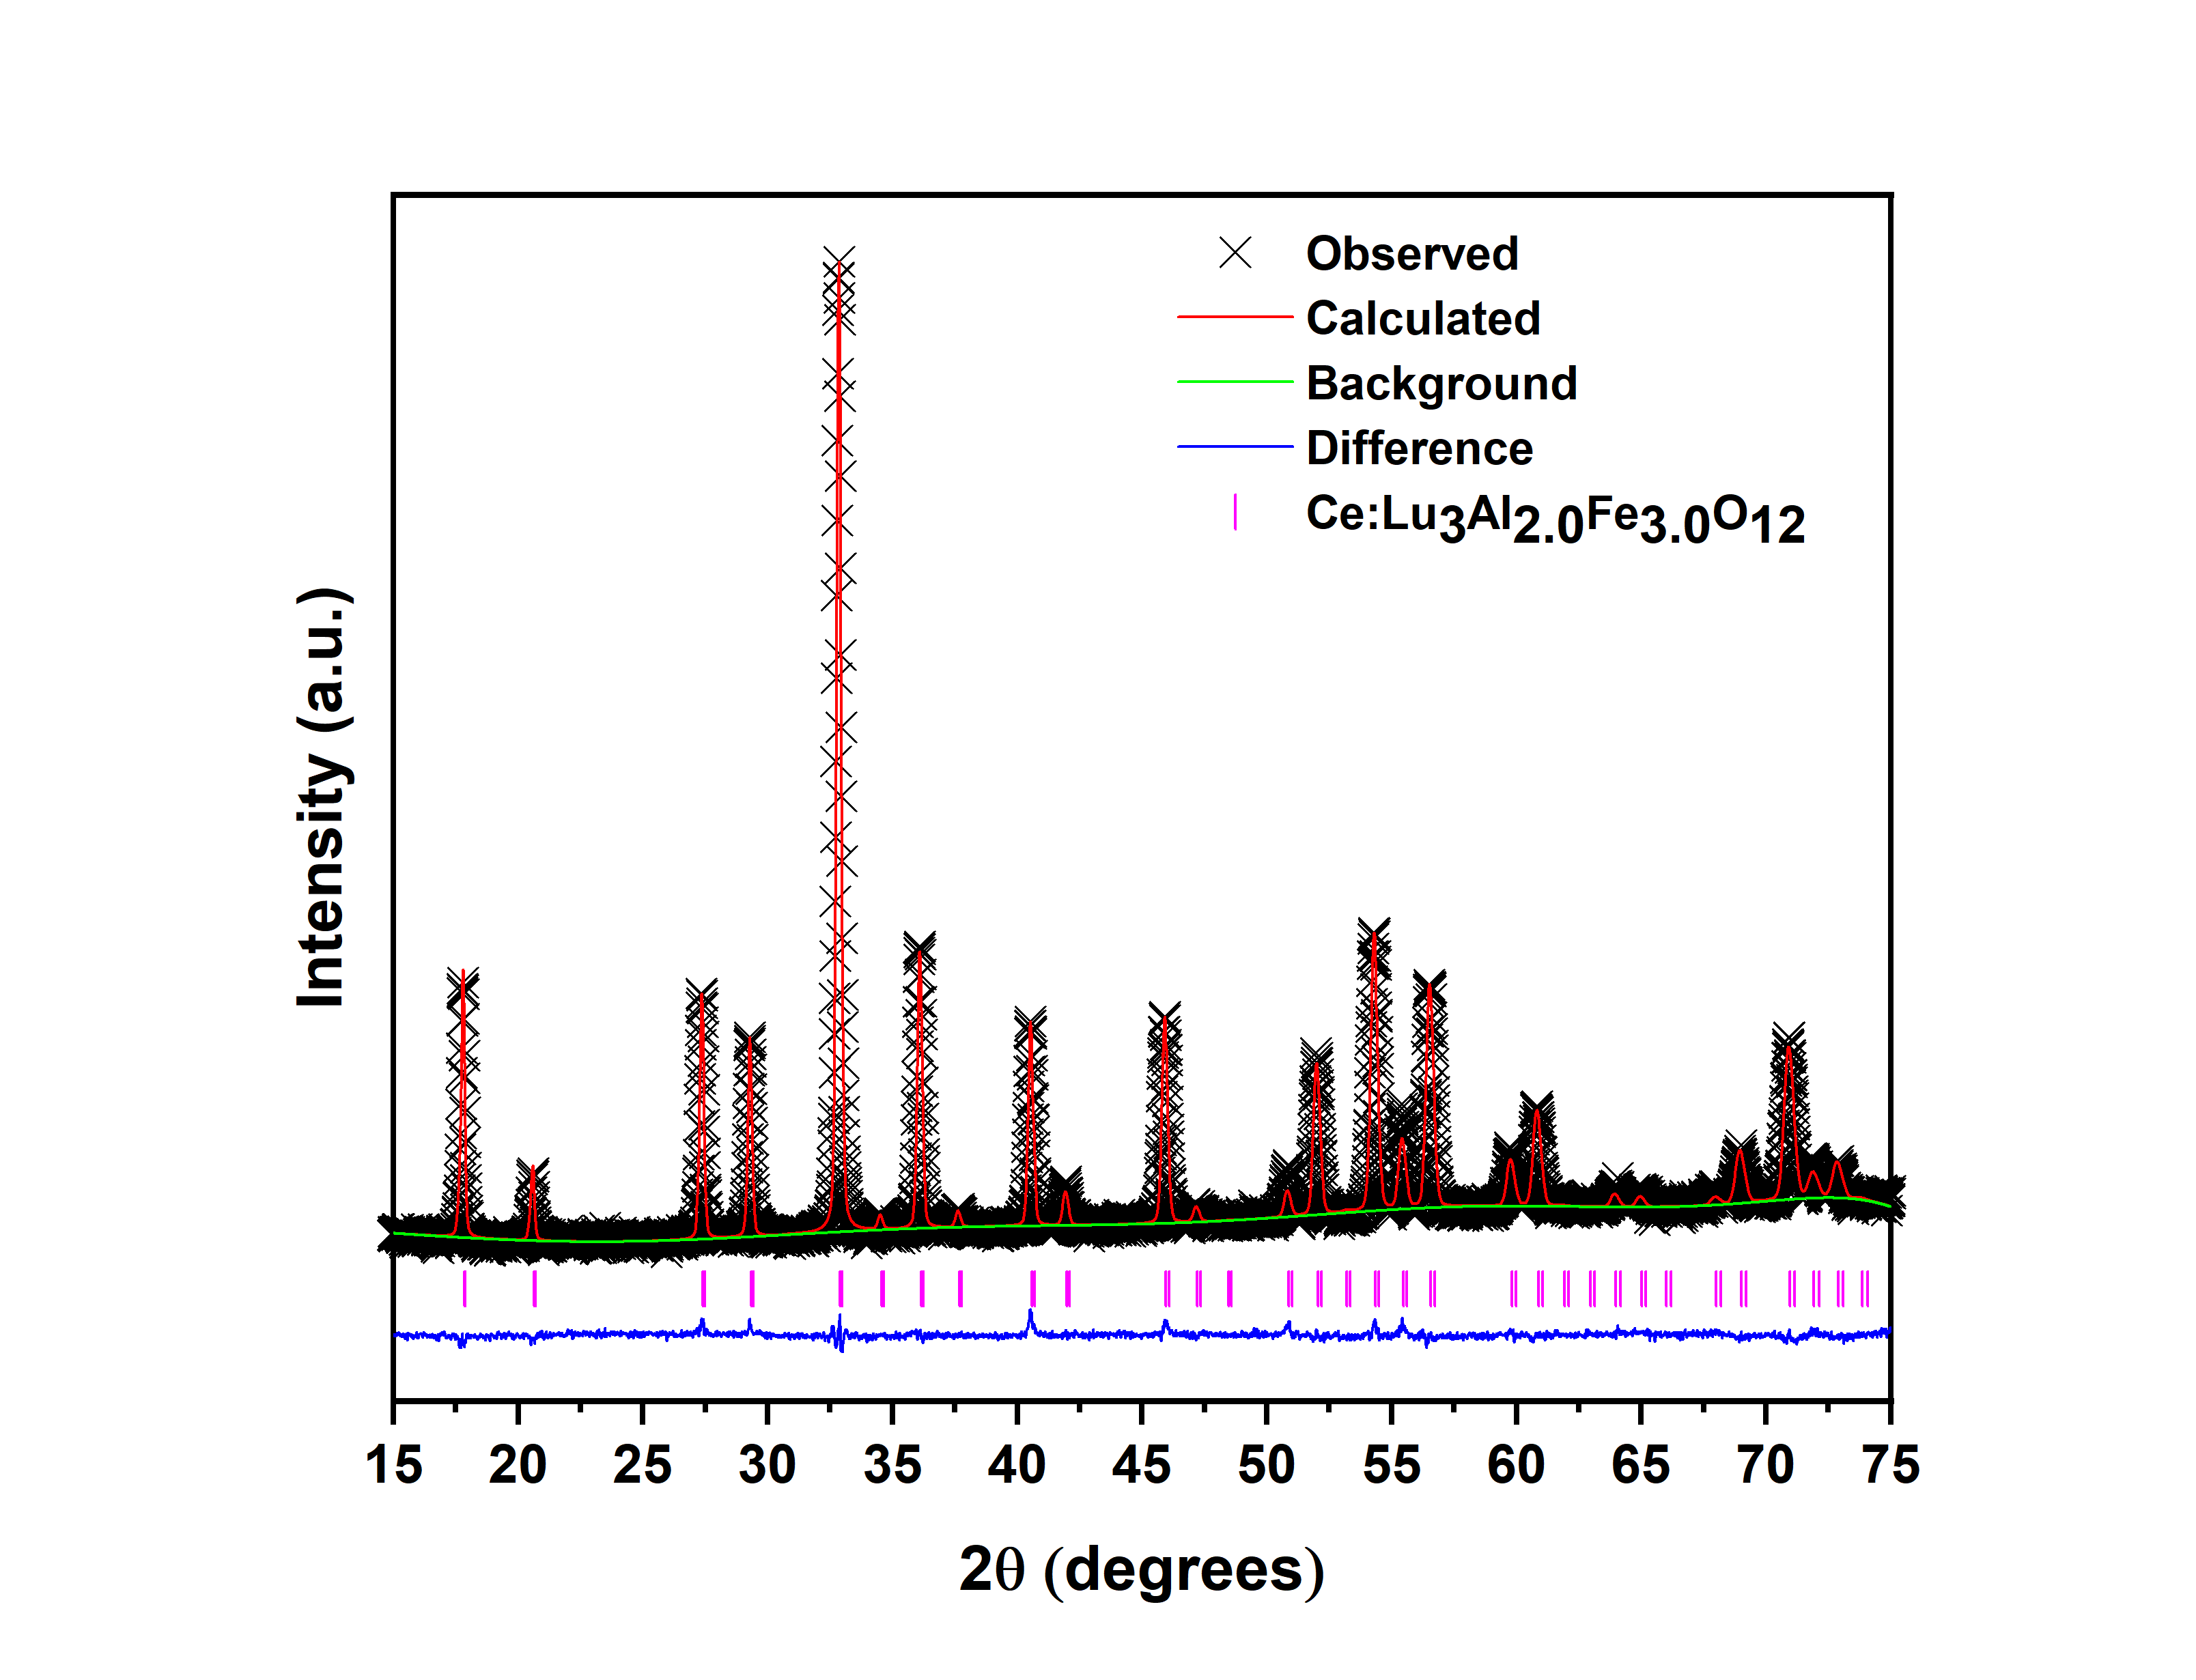
\includegraphics[width=11cm]{Anexos/x30.png}%
		\caption{Resultados de refinamiento Rietveld de
		\ce{Lu_{3.0}Al_{2.0}Fe_{3.0}O12}}\label{fig:refi30}
	\end{figure}

	\begin{figure}[h]
		\centering%
		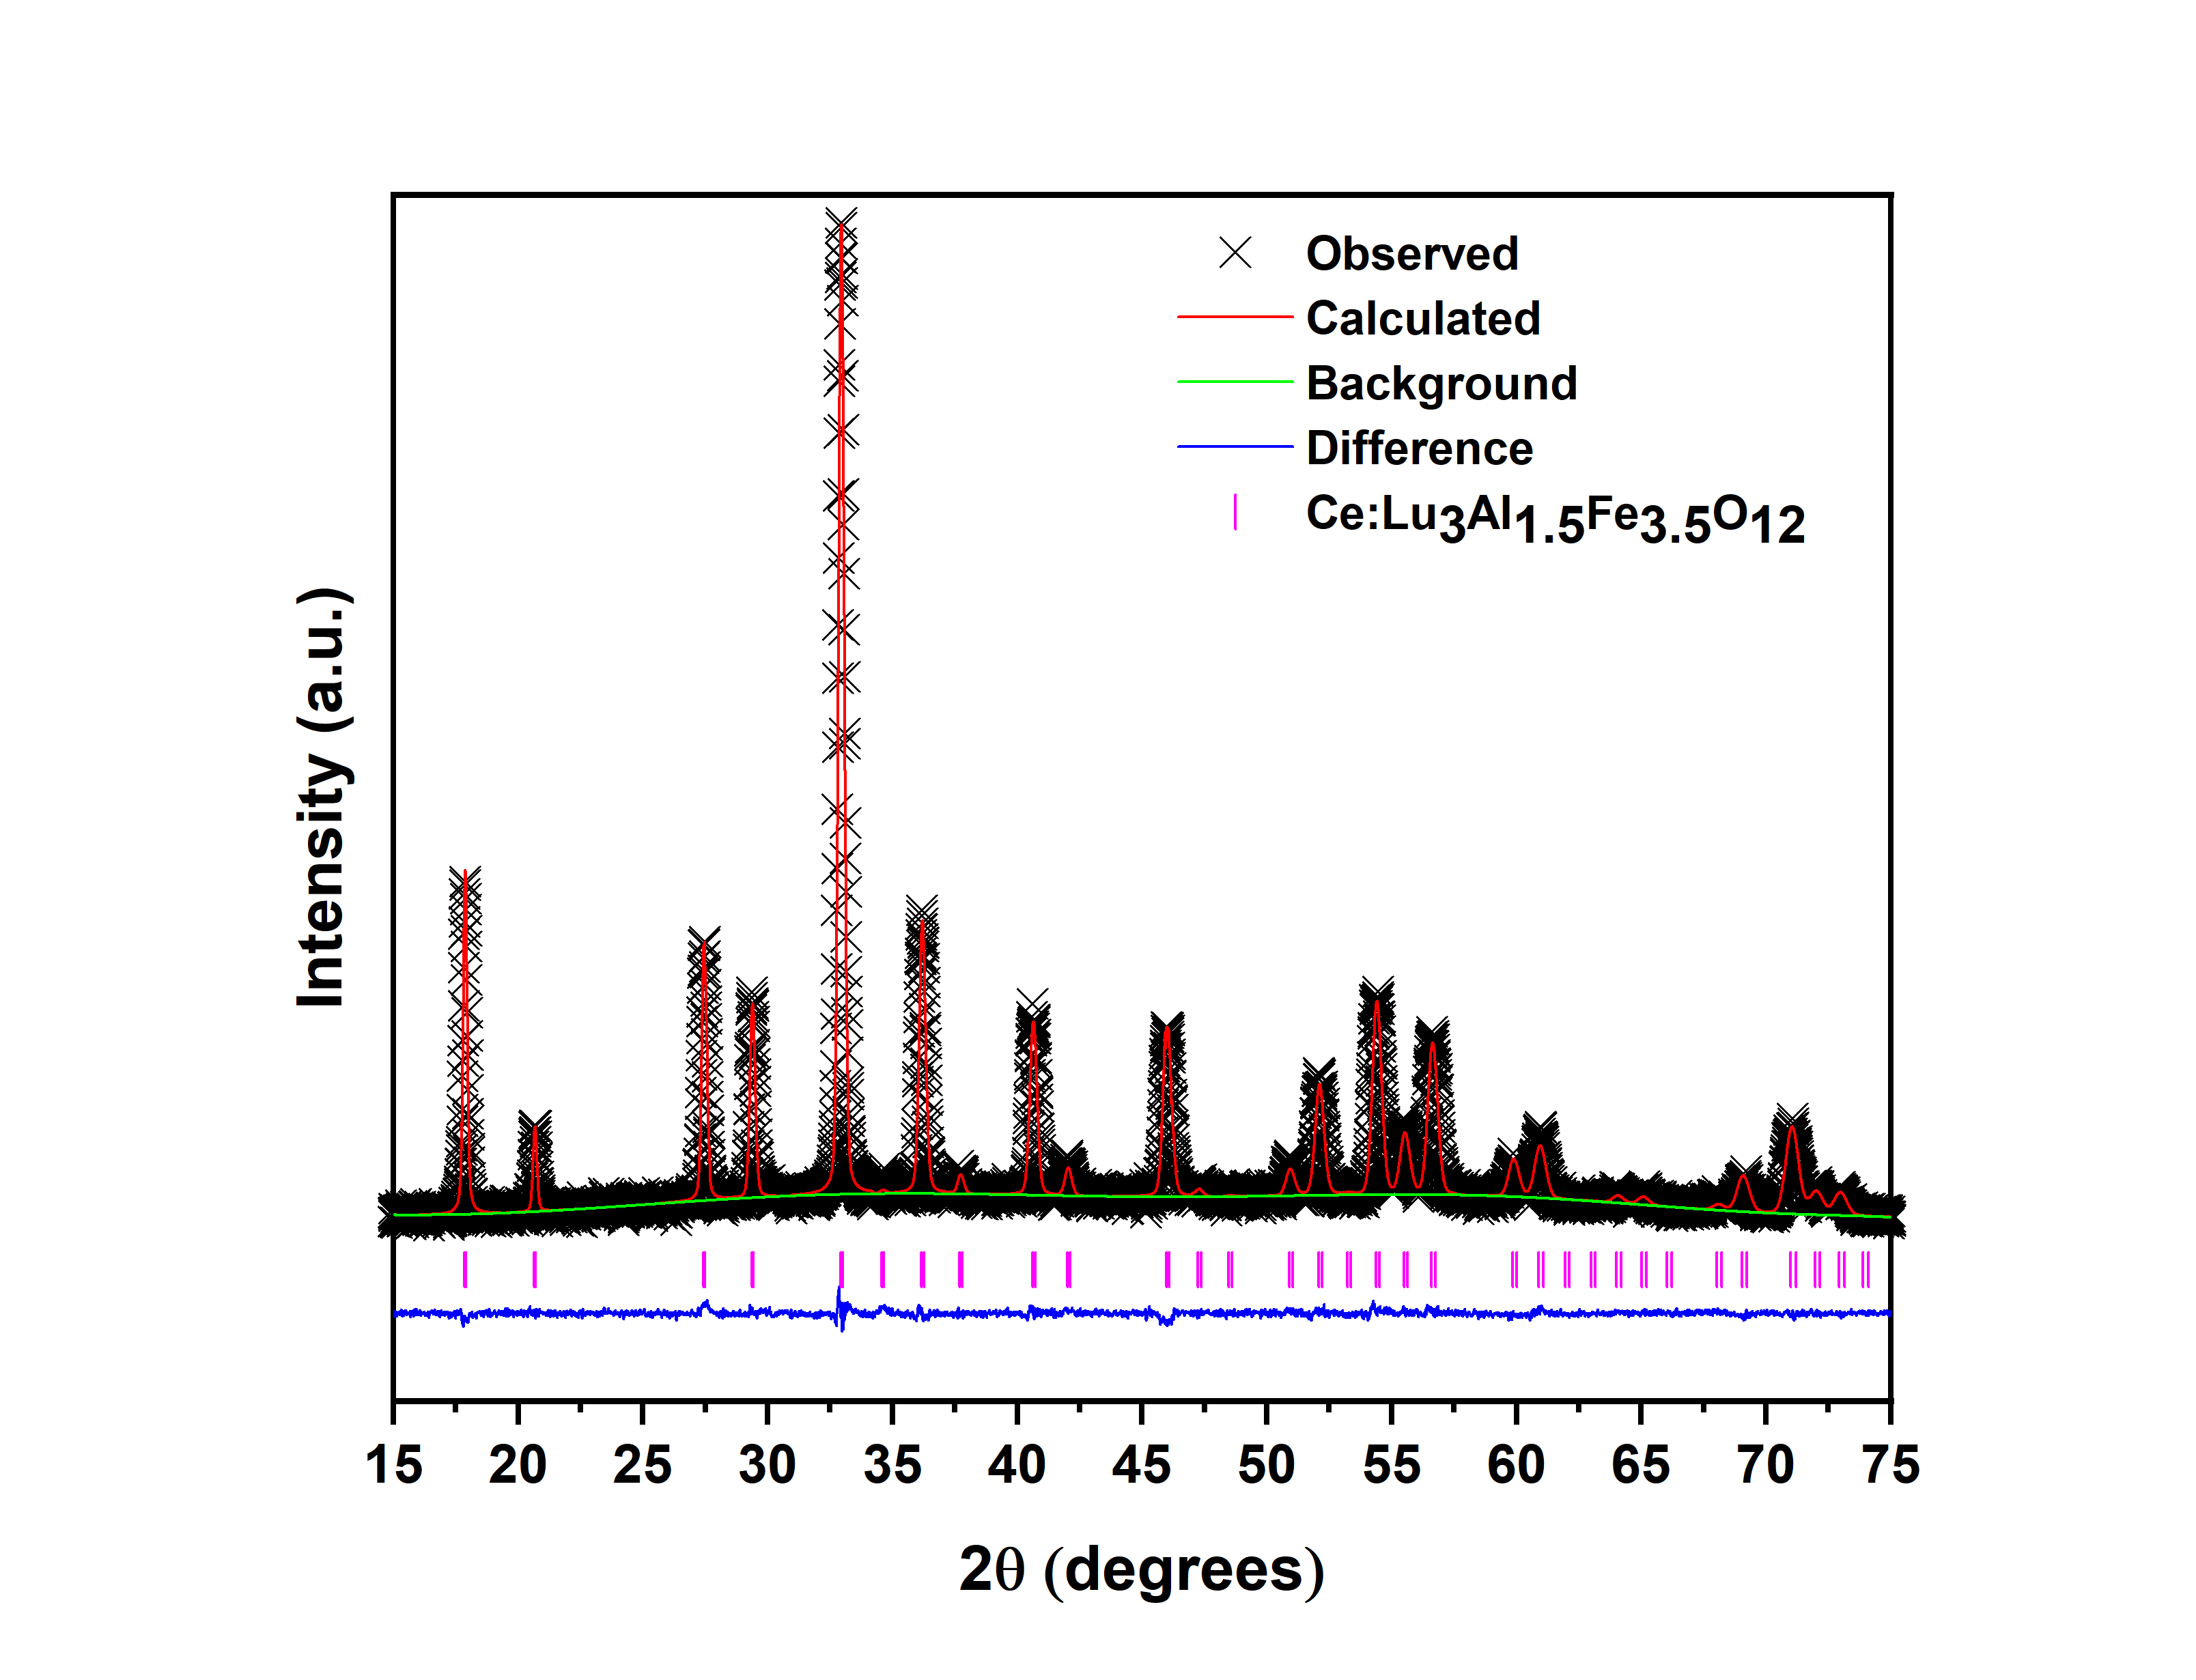
\includegraphics[width=11cm]{Anexos/x35.png}%
		\caption{Resultados de refinamiento Rietveld de
		\ce{Lu_{3.0}Al_{1.5}Fe_{3.5}O12}}\label{fig:refi35}
	\end{figure}

	\begin{figure}[h]
		\centering%
		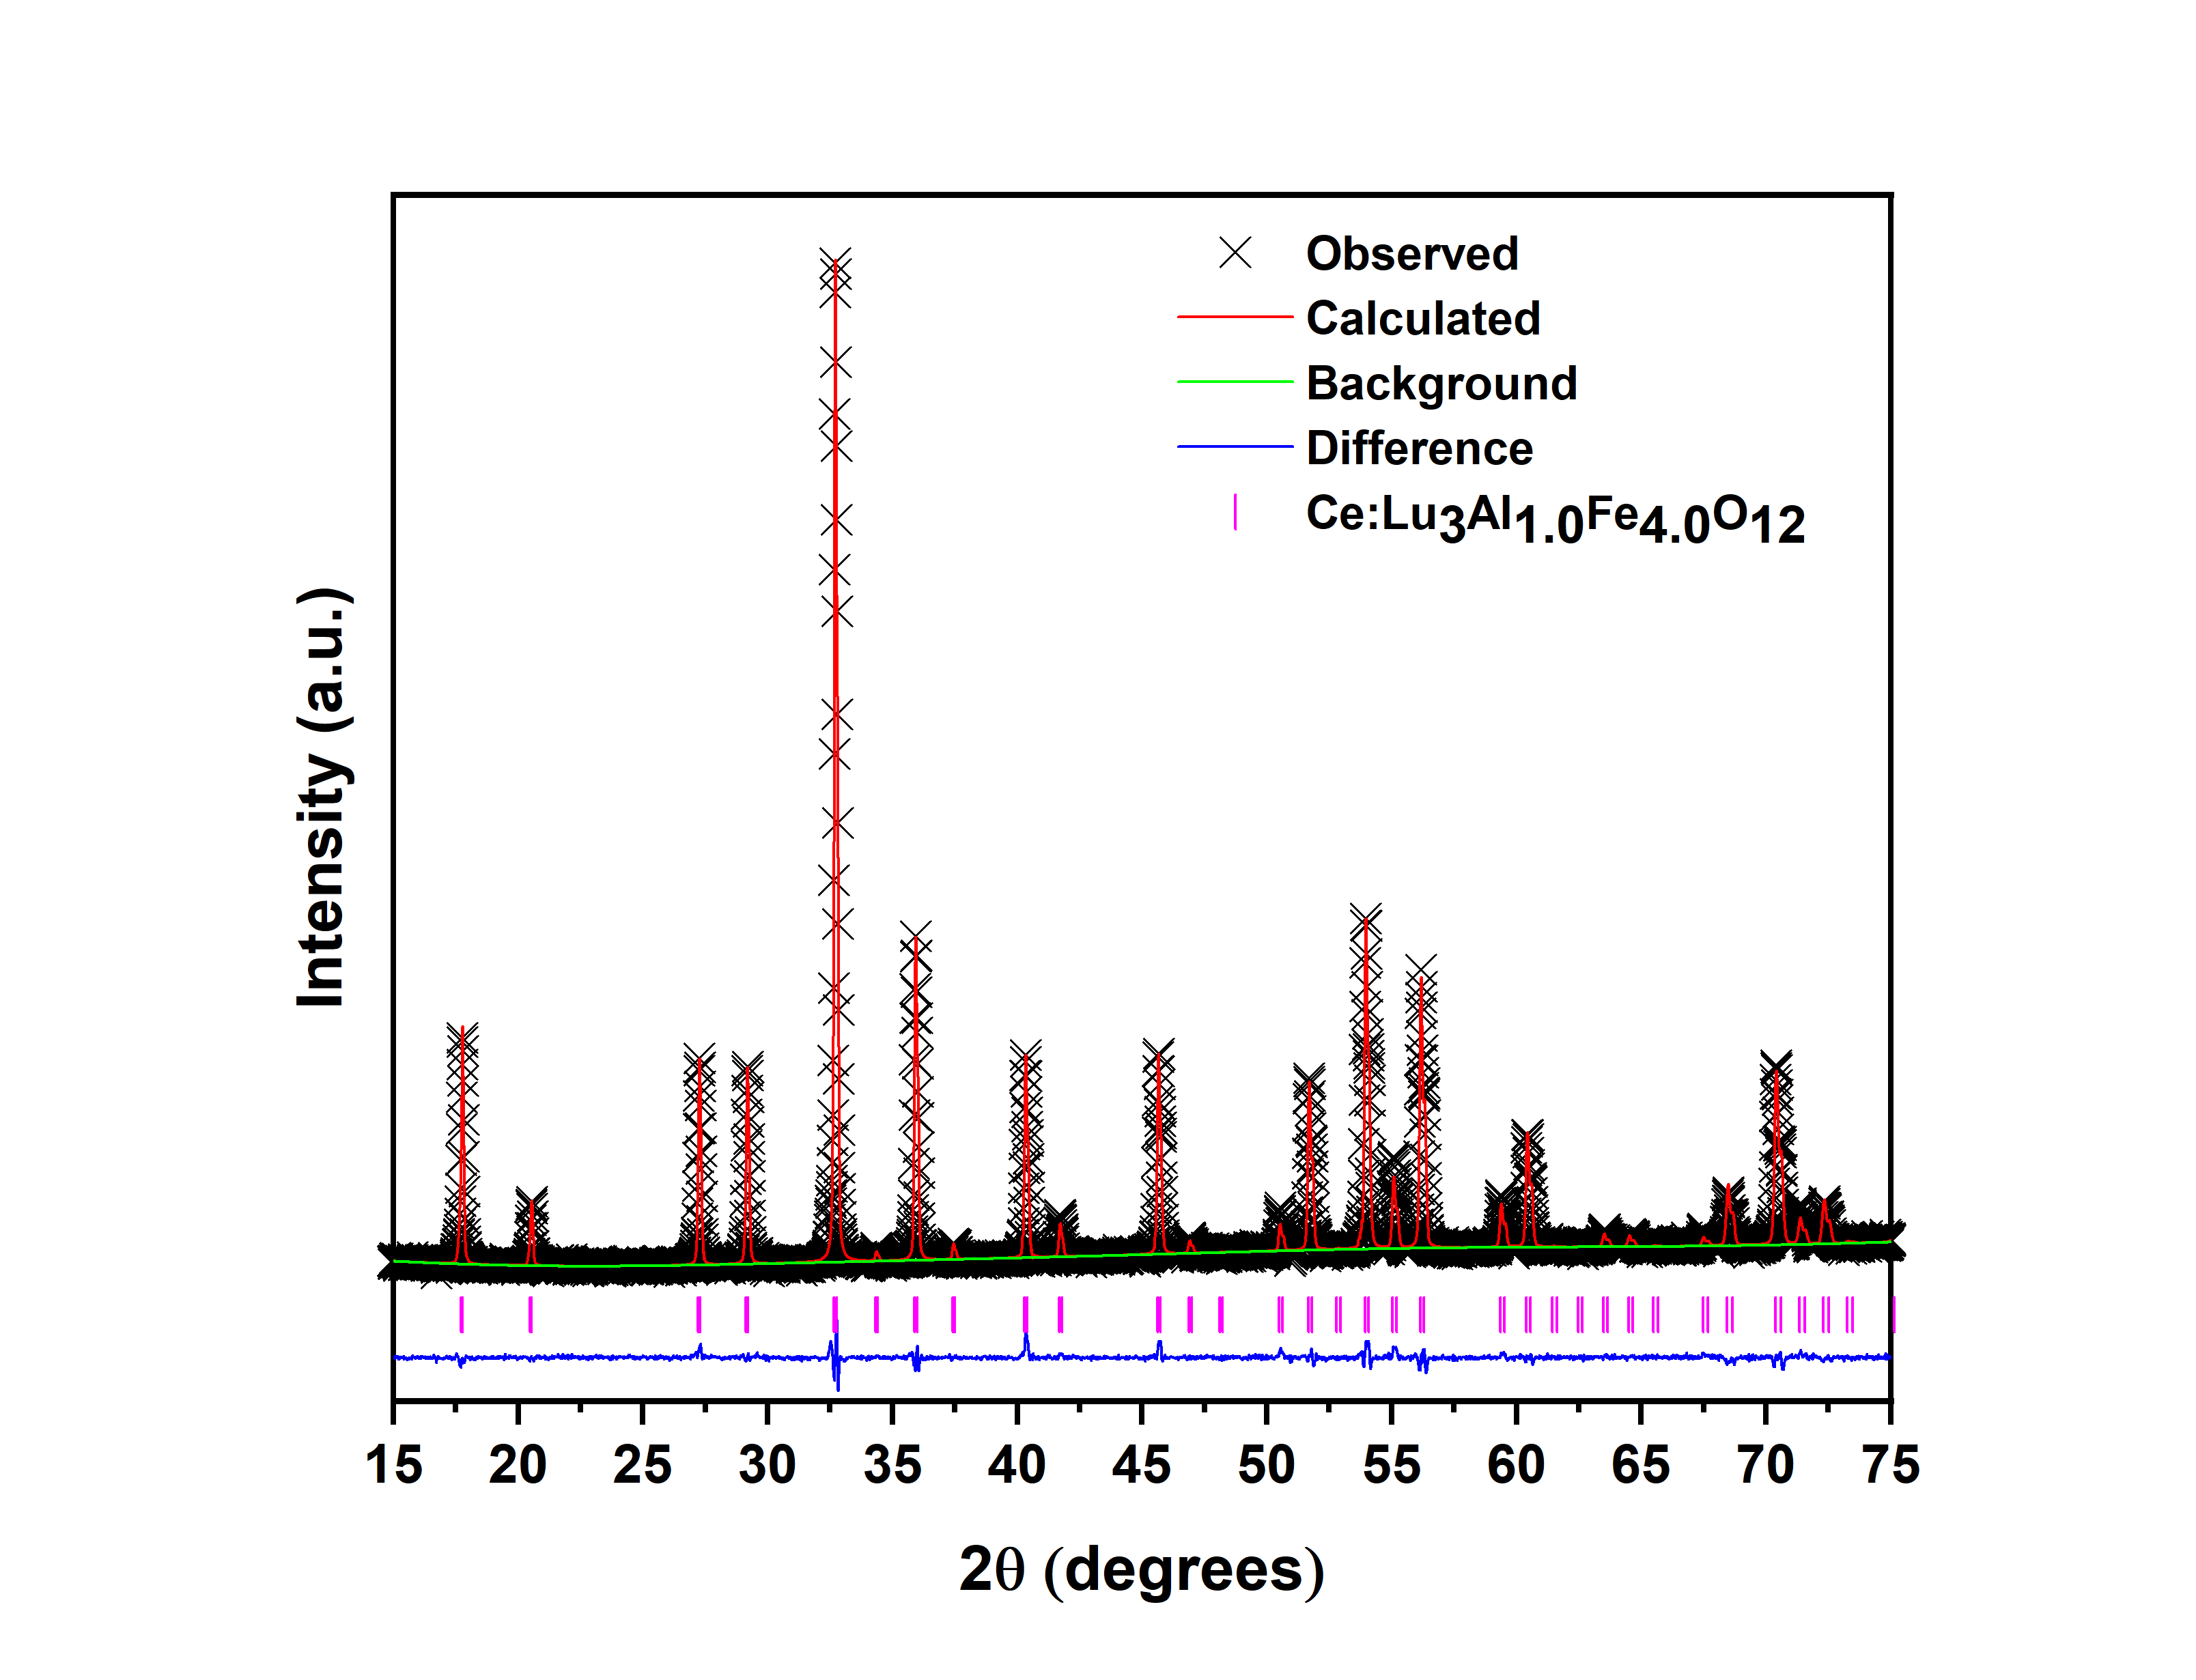
\includegraphics[width=11cm]{Anexos/x40.png}%
		\caption{Resultados de refinamiento Rietveld de
		\ce{Lu_{3.0}Al_{1.0}Fe_{4.0}O12}}\label{fig:refi40}
	\end{figure}

	\begin{figure}[t!]
		\centering%
		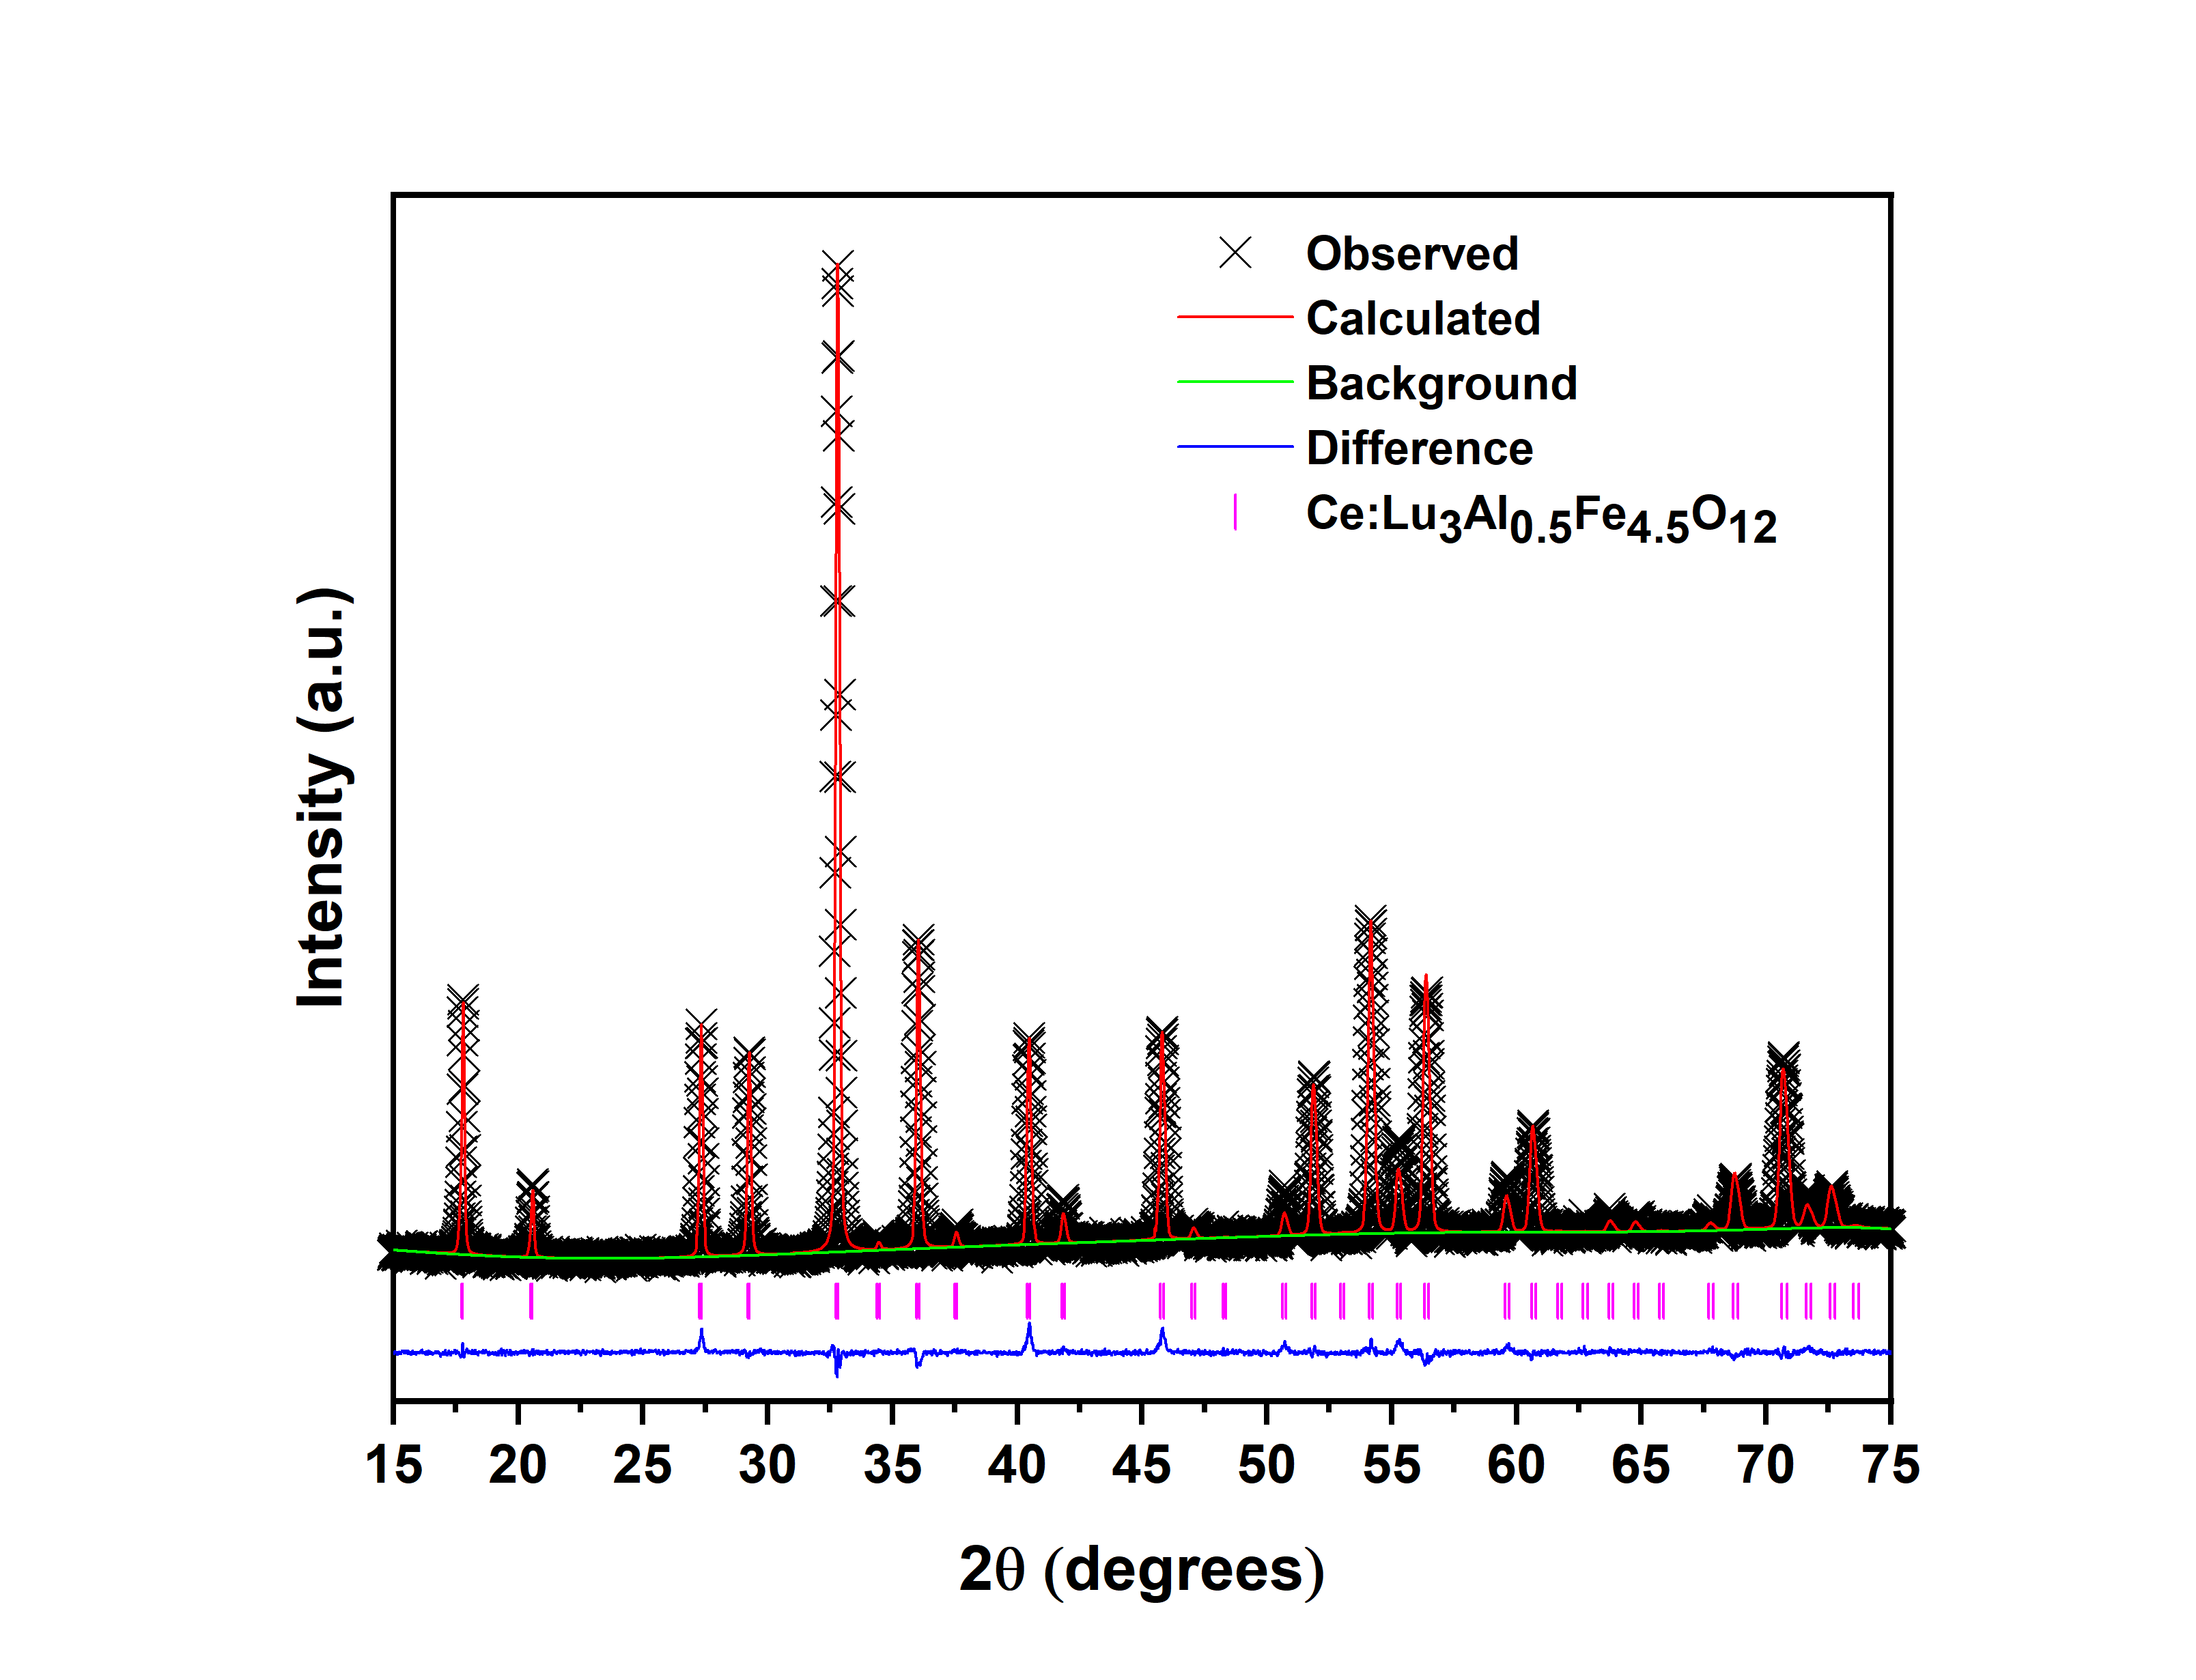
\includegraphics[width=11cm]{Anexos/x45.png}%
		\caption{Resultados de refinamiento Rietveld de
		\ce{Lu_{3.0}Al_{0.5}Fe_{4.5}O12}}\label{fig:refi45}
	\end{figure}

	\chapter{Microscopia Electrónica de Barrido}\label{AnexoC}

	\begin{figure}[h]
		\centering%

		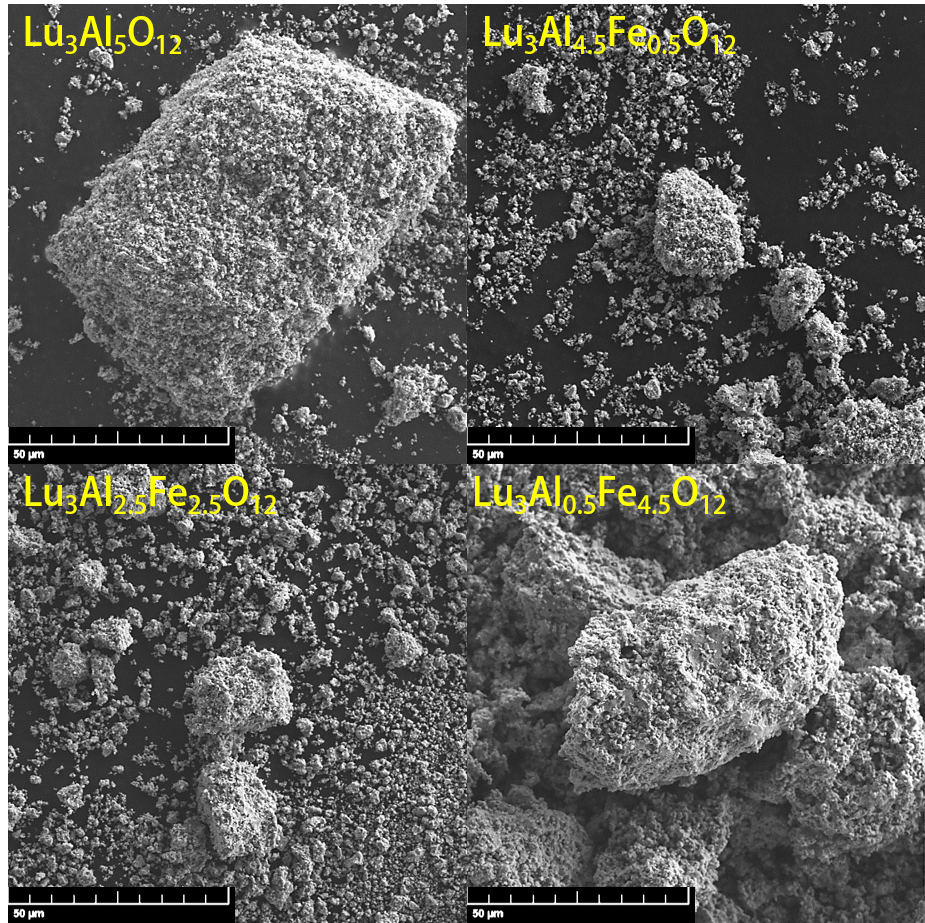
\includegraphics[width=12cm]{Kap5/sec2k.png}%
		\caption{Microscopia con electrones secundarios a 2.000 aumentos de los
		materiales \ce{Lu_{3.0}Al_{0.5}Fe_{4.5}O12} con x=0.0, 0.5, 2.5 y
		4.5}\label{fig:sec2}
	\end{figure}

	\begin{figure}[h]
		\centering%

		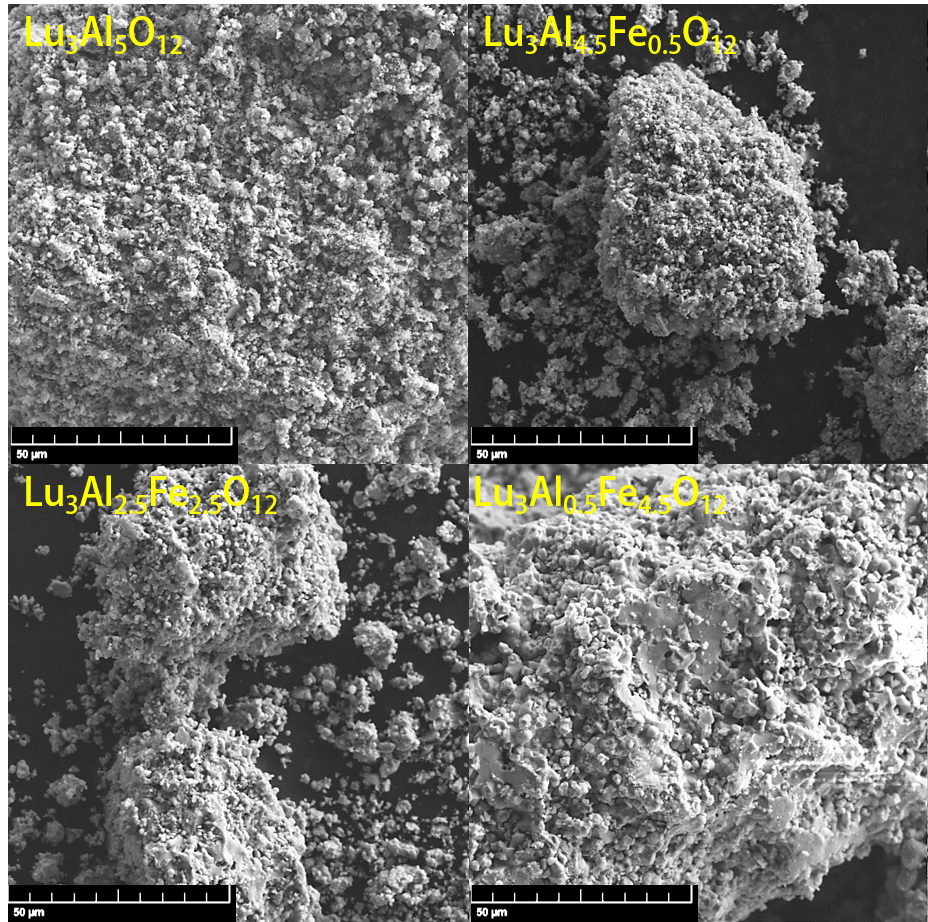
\includegraphics[width=\textwidth]{Kap5/sec5k.png}%
		\caption{Microscopia con electrones secundarios a 5.000 aumentos de los
		materiales \ce{Lu_{3.0}Al_{0.5}Fe_{4.5}O12} con x=0.0, 0.5, 2.5 y
		4.5}\label{fig:sec5}
	\end{figure}

	\begin{figure}[h]
		\centering%

		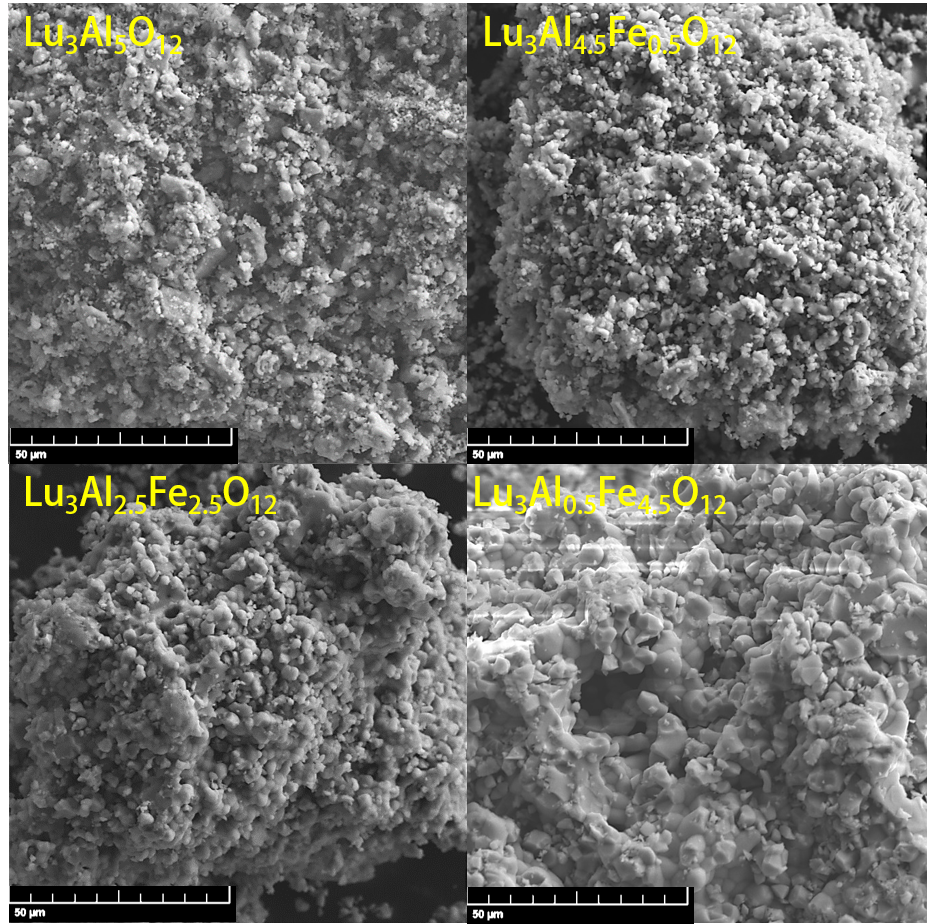
\includegraphics[width=\textwidth]{Kap5/sec10k.png}%
		\caption{Microscopia con electrones secundarios a 10.000 aumentos de los
		materiales \ce{Lu_{3.0}Al_{0.5}Fe_{4.5}O12} con x=0.0, 0.5, 2.5 y
		4.5}\label{fig:sec10}
	\end{figure}

	\begin{figure}[h]
		\centering%

		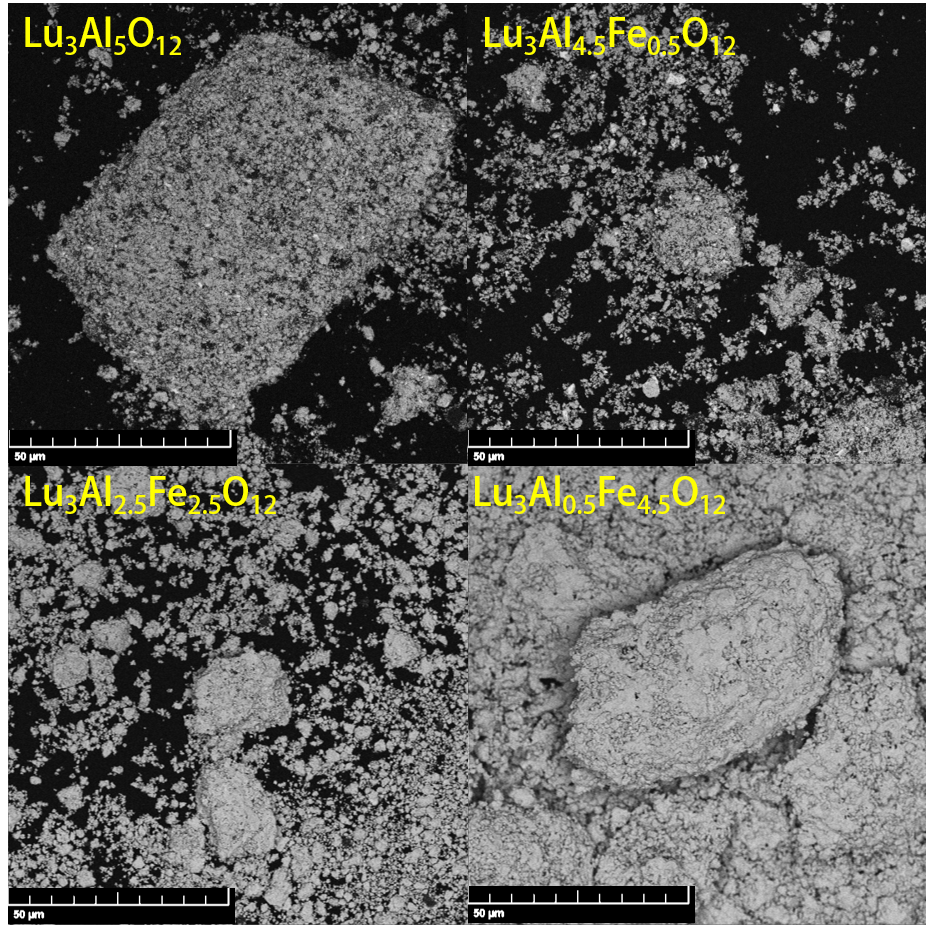
\includegraphics[width=\textwidth]{Kap5/ret2k.png}%
		\caption{Microscopia con electrones retrodispersados a 2.000 aumentos de los
		materiales \ce{Lu_{3.0}Al_{0.5}Fe_{4.5}O12} con x=0.0, 0.5, 2.5 y
		4.5}\label{fig:ret2}
	\end{figure}

	\begin{figure}[h]
		\centering%

		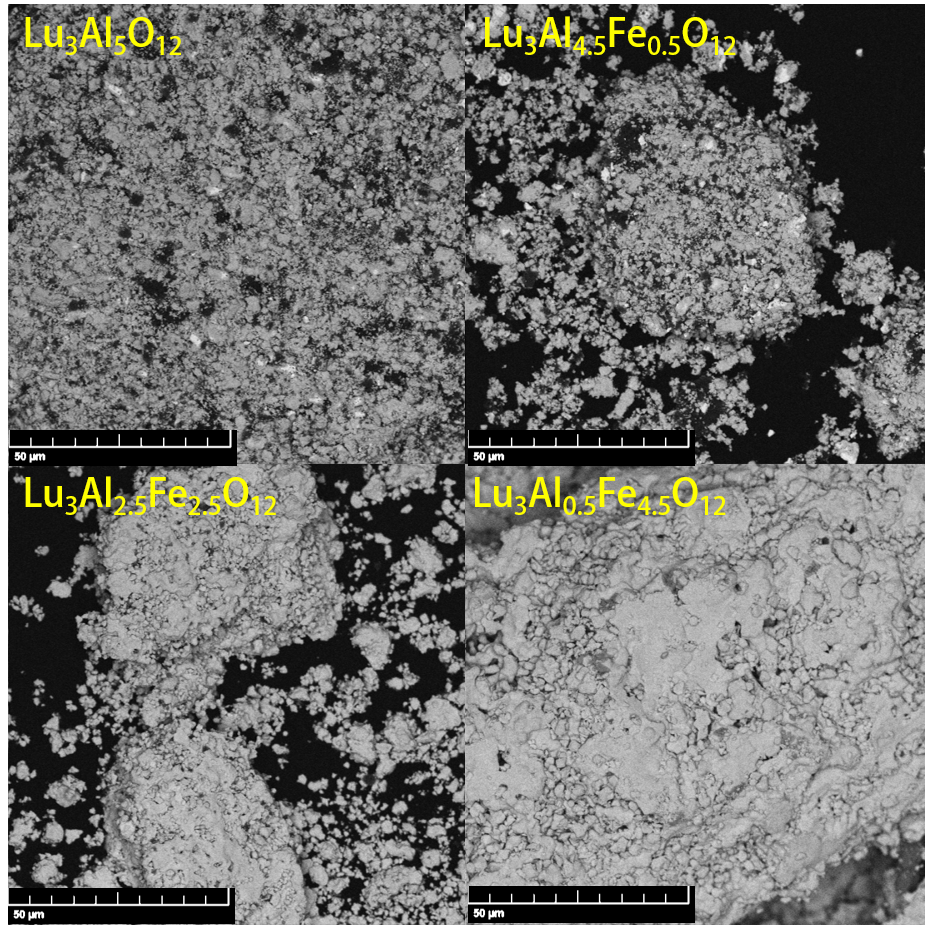
\includegraphics[width=\textwidth]{Kap5/ret5k.png}%
		\caption{Microscopia con electrones retrodispersados a 5.000 aumentos de los
		materiales \ce{Lu_{3.0}Al_{0.5}Fe_{4.5}O12} con x=0.0, 0.5, 2.5 y
		4.5}\label{fig:ret5}
	\end{figure}

	\begin{figure}[h]
		\centering%

		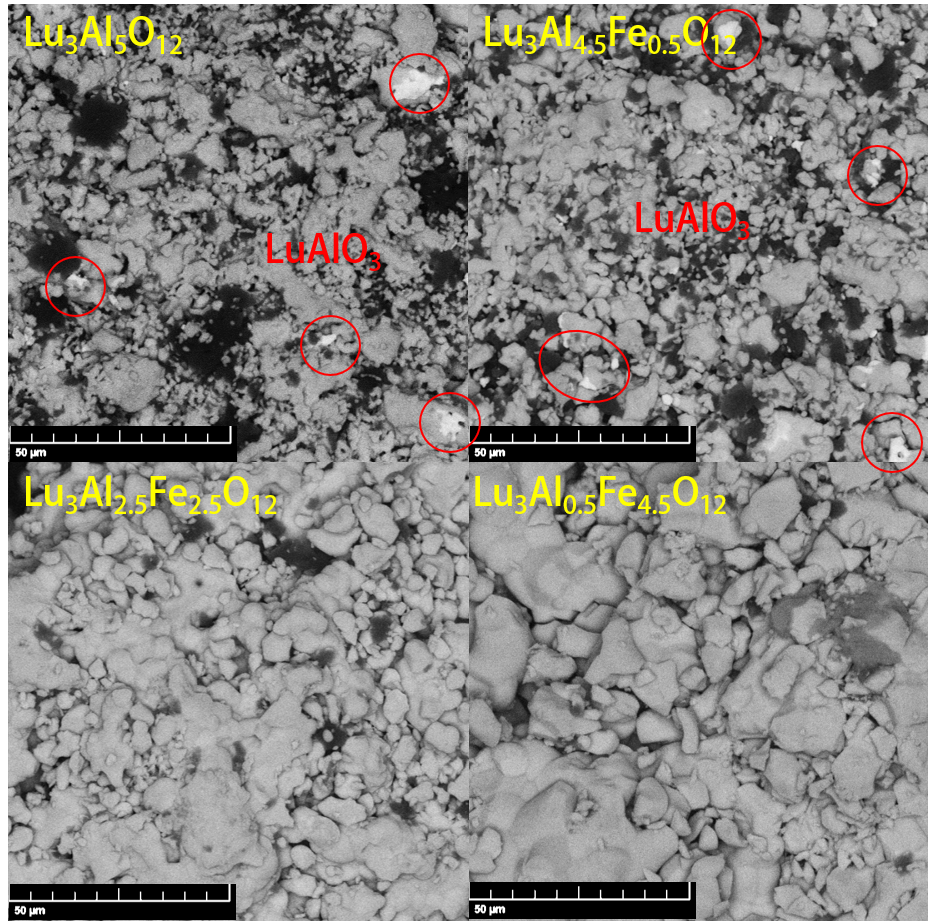
\includegraphics[width=\textwidth]{Kap5/ret20k.png}%
		\caption{Microscopia con electrones retrodispersados a 20.000 aumentos de los
		materiales \ce{Lu_{3.0}Al_{0.5}Fe_{4.5}O12} con x=0.0, 0.5, 2.5 y
		4.5}\label{fig:ret20}
	\end{figure}

	\begin{figure}[h]
		\centering%

		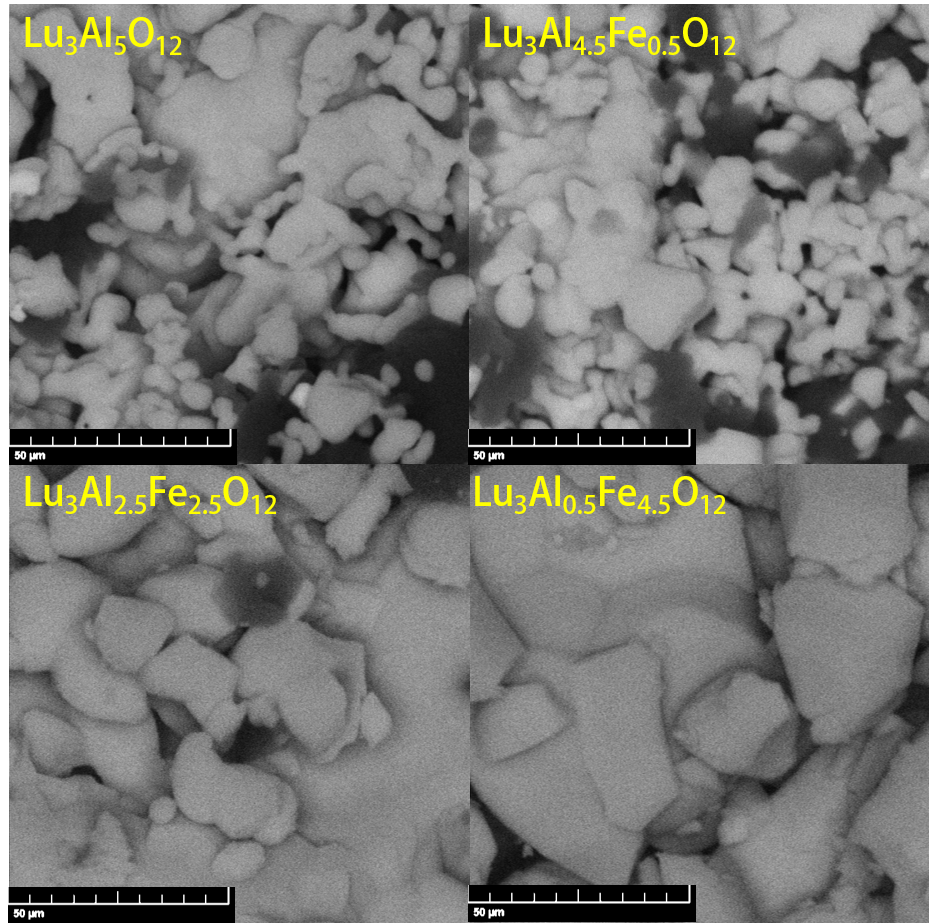
\includegraphics[width=\textwidth]{Kap5/ret90k.png}%
		\caption{Microscopia con electrones retrodispersados a 2.000 aumentos de los
		materiales \ce{Lu_{3.0}Al_{0.5}Fe_{4.5}O12} con x=0.0, 0.5, 2.5 y
		4.5}\label{fig:ret90}
	\end{figure}

	\chapter{Tamaño de Partícula}\label{AnexoD}

	\begin{figure}[h]
		\centering%

		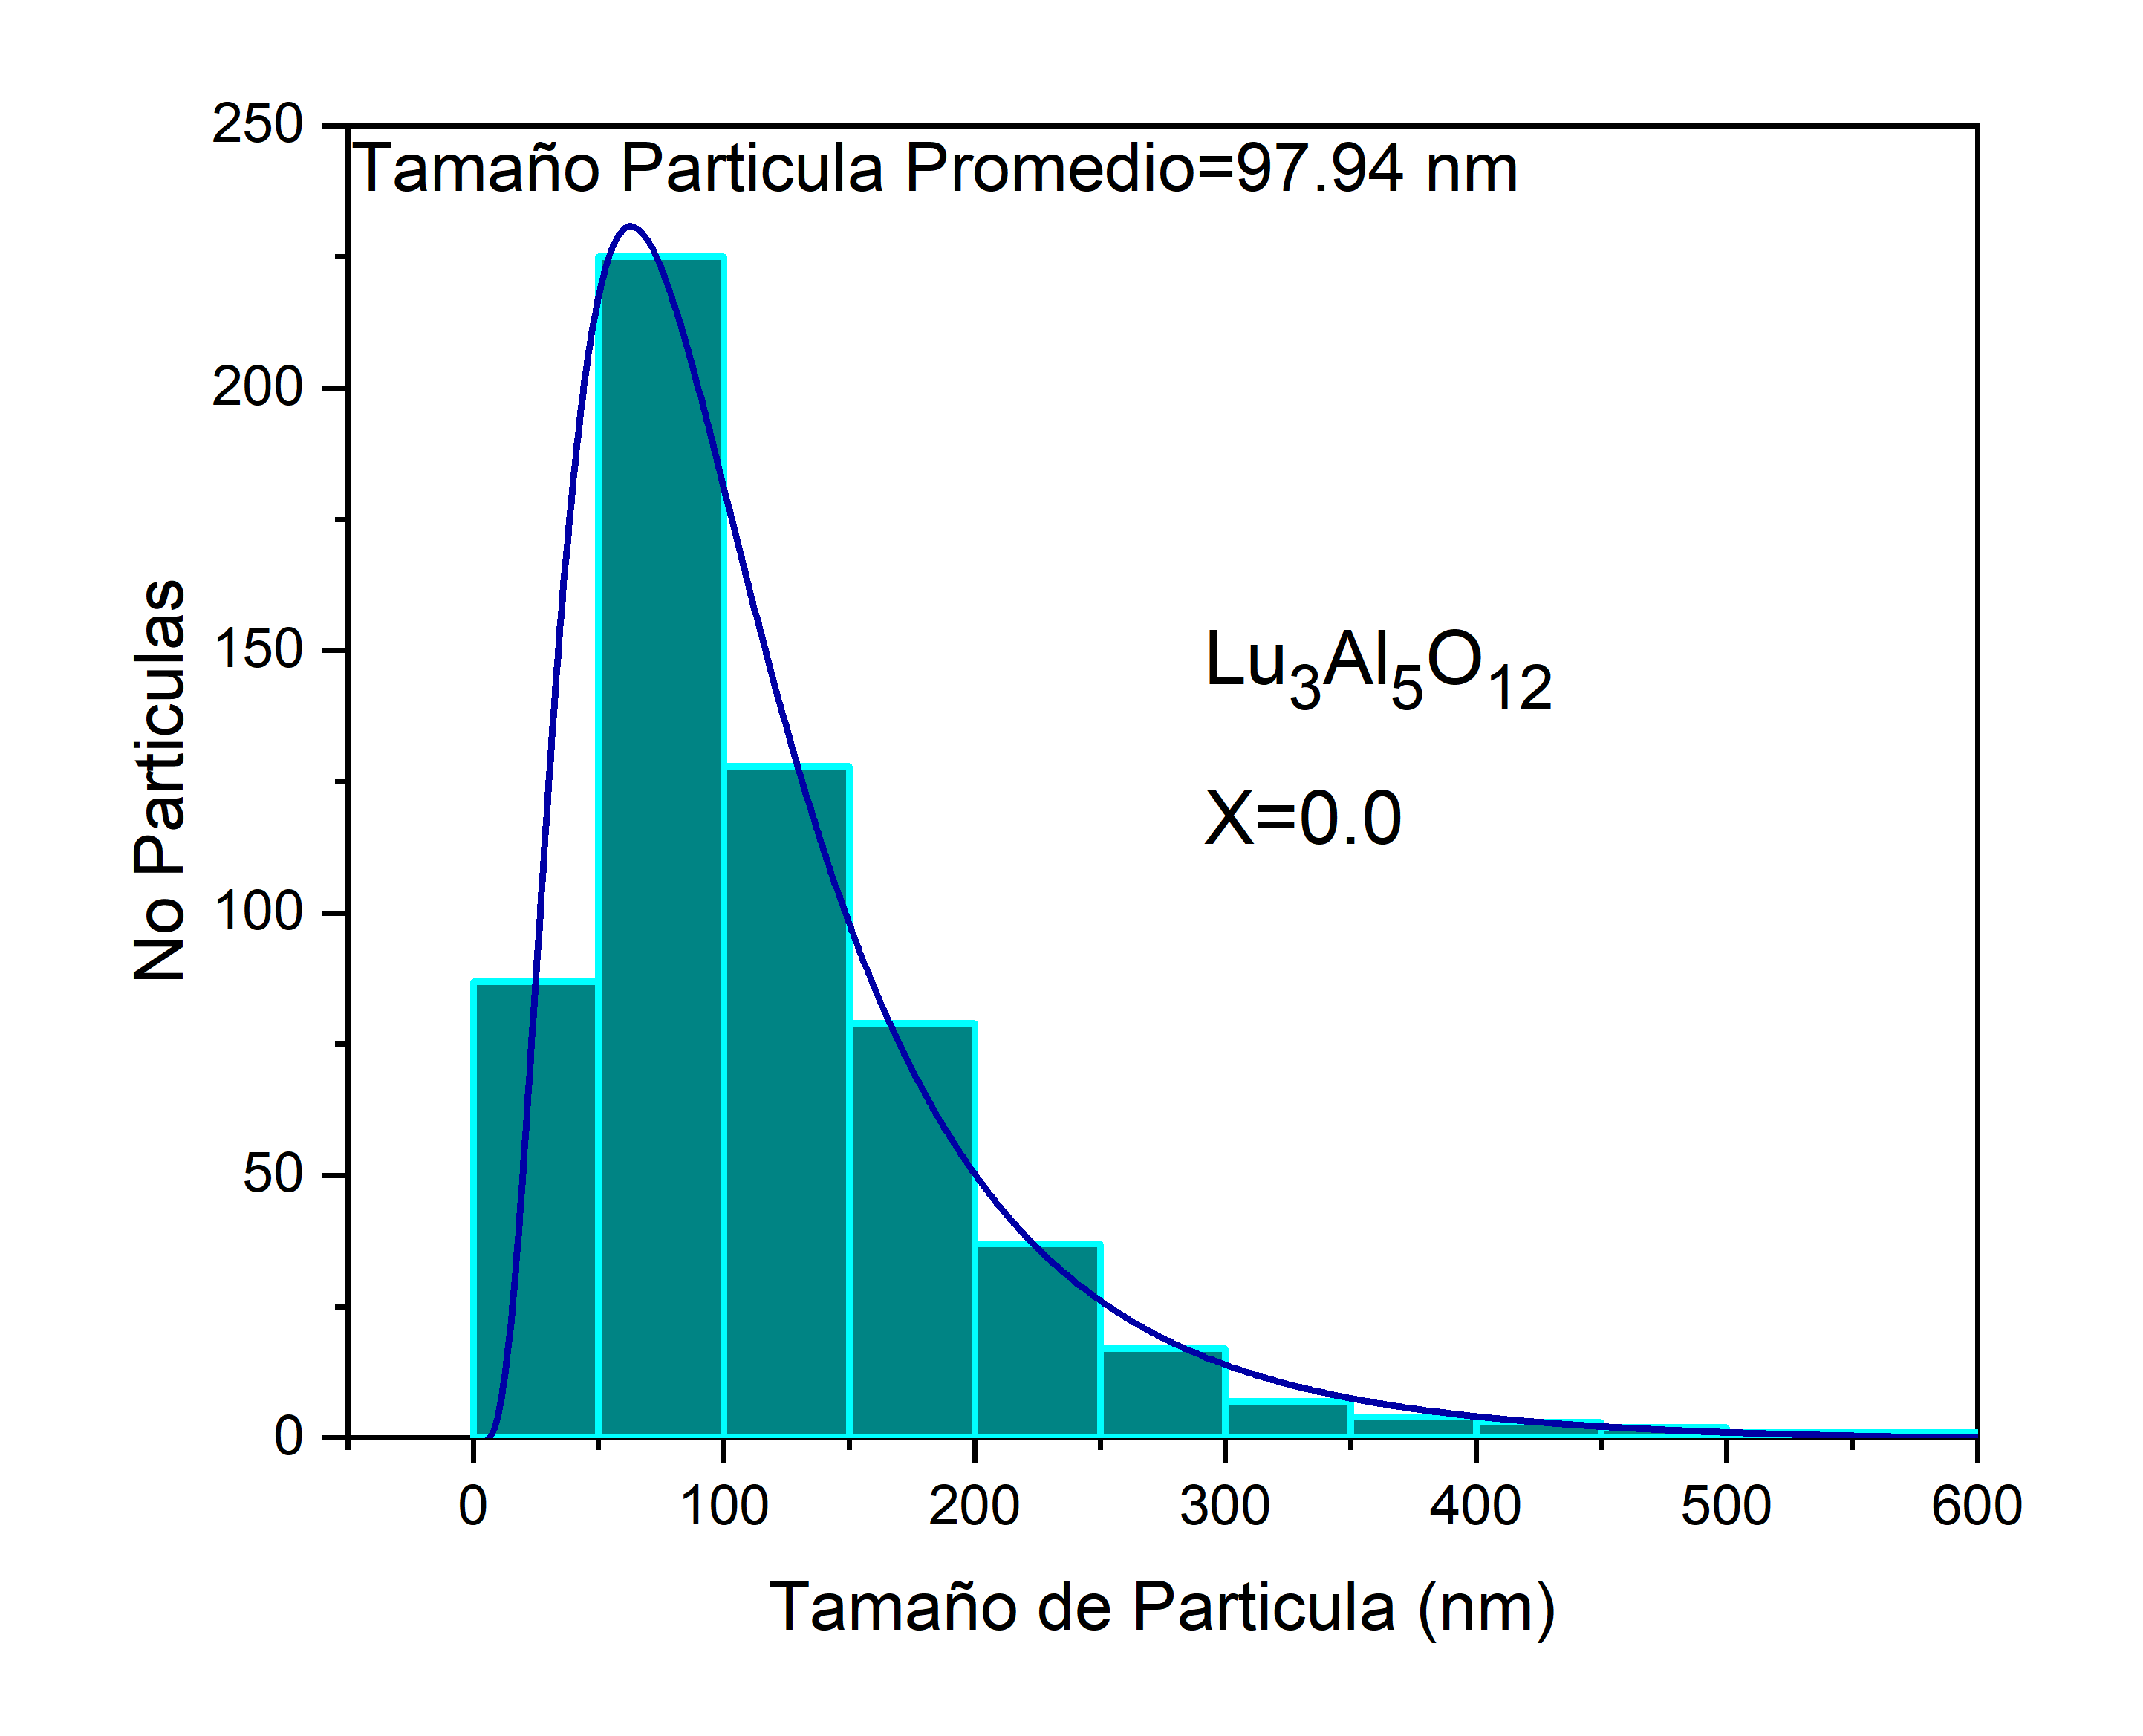
\includegraphics[width=13cm]{Kap5/TamG0.png}%
		\caption{Distribución del tamaño de partícula para \ce{Lu_{3.0}Al_{5.0}O12} medida mediante ImageJ}\label{fig:tamG0}
	\end{figure}

	\begin{figure}[h]
		\centering%

		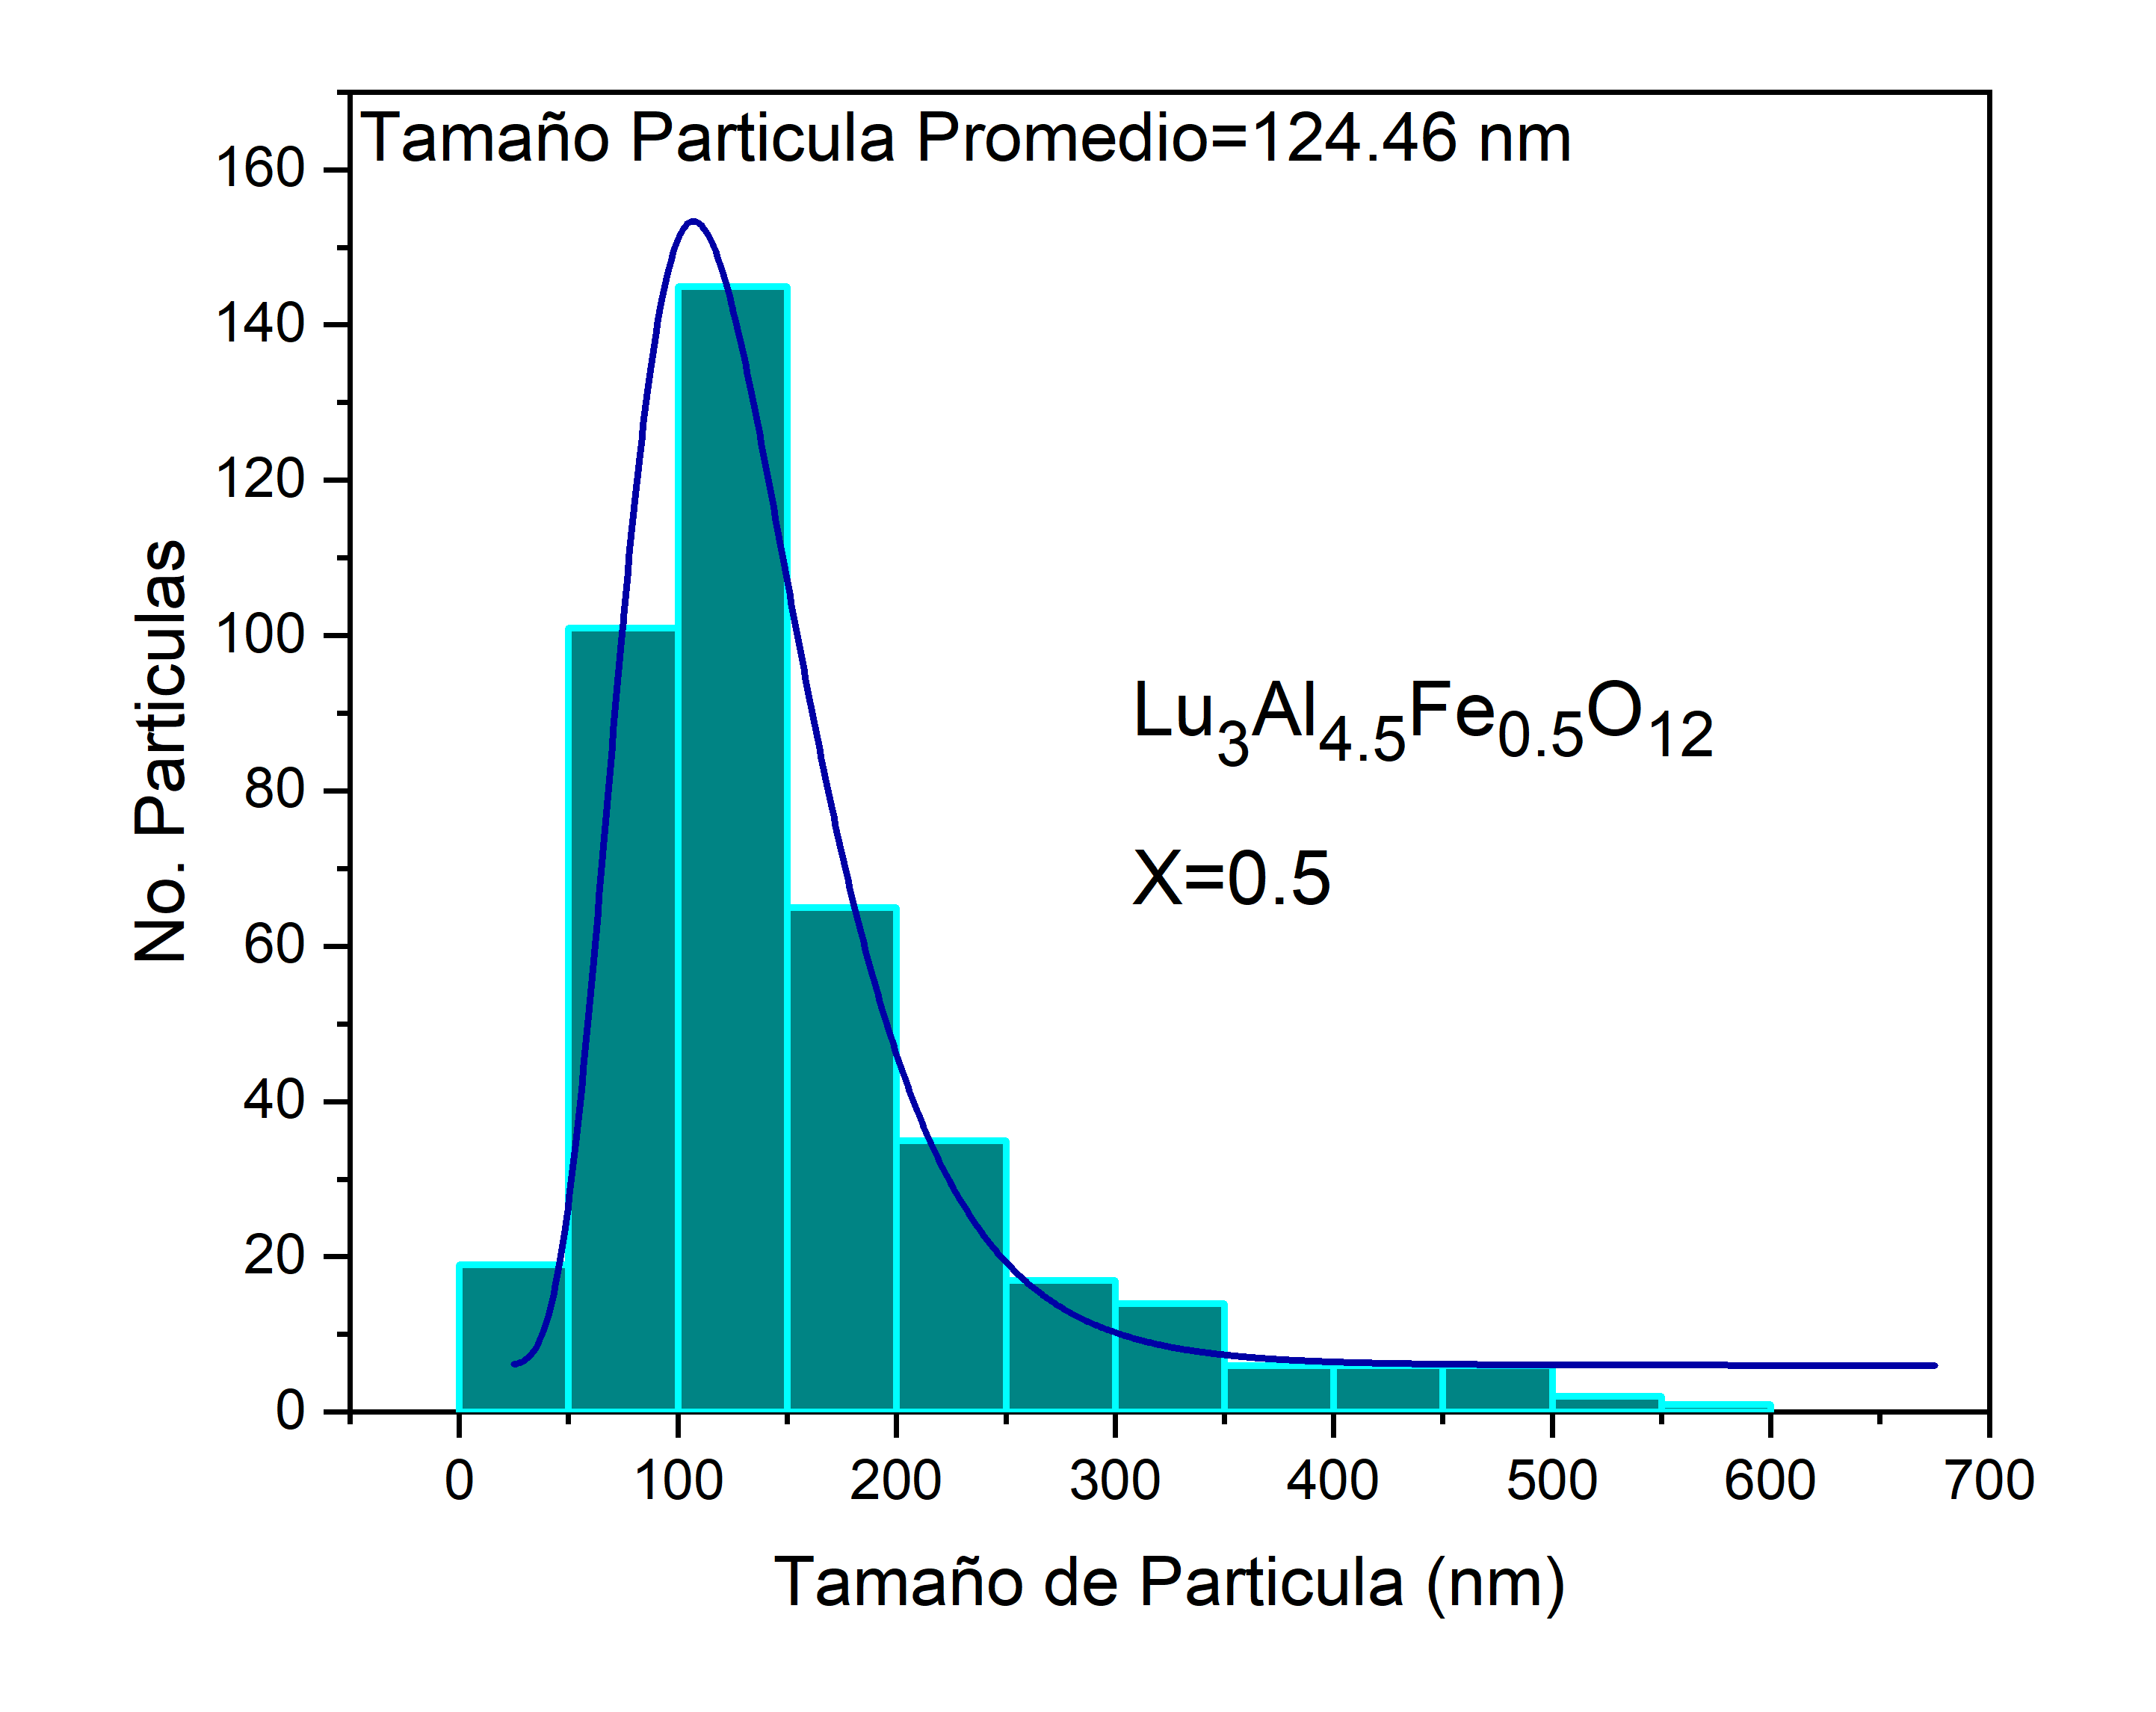
\includegraphics[width=\textwidth]{Kap5/TamG1.png}%
		\caption{Distribución del tamaño de partícula para \ce{Lu_{3.0}Al_{4.5}Fe_{0.5}O12} medida mediante ImageJ}\label{fig:tamG1}
	\end{figure}

	\begin{figure}[h]
		\centering%

		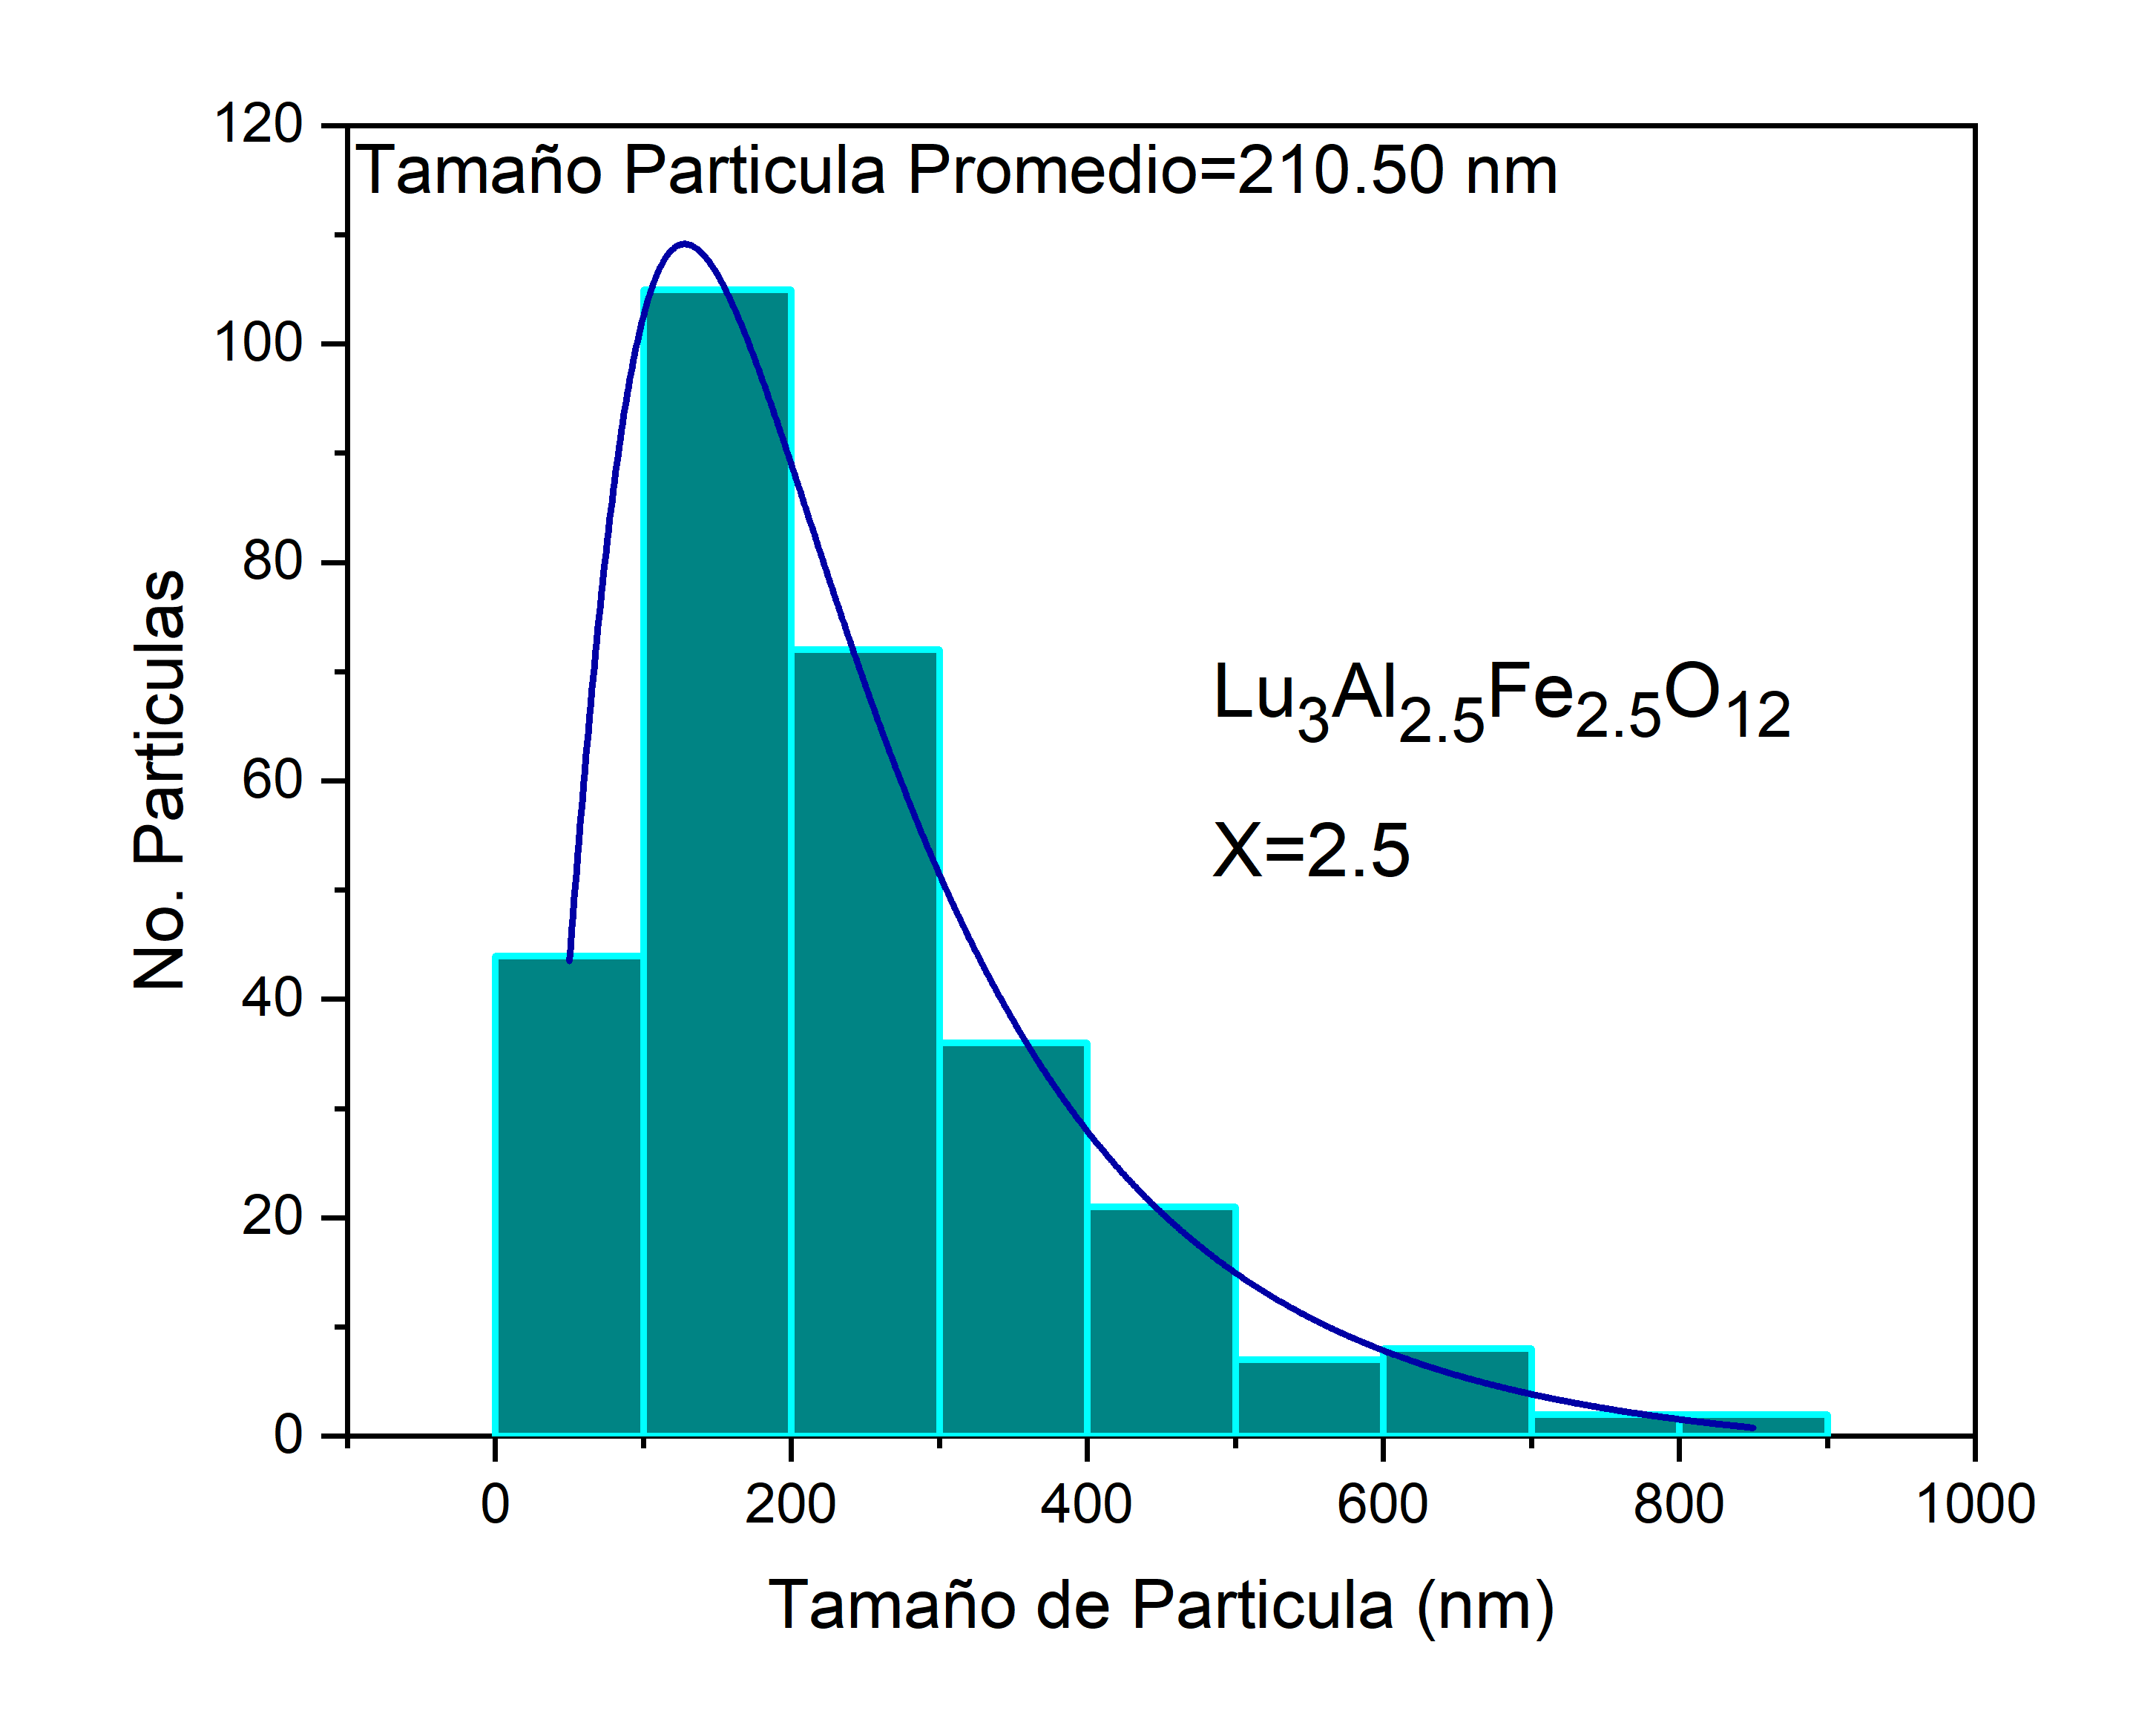
\includegraphics[width=\textwidth]{Kap5/TamG5.png}%
		\caption{Distribución del tamaño de partícula para \ce{Lu_{3.0}Al_{2.5}Fe_{2.5}O12} medida mediante ImageJ}\label{fig:tamG5}
	\end{figure}

	\begin{figure}[h]
		\centering%

		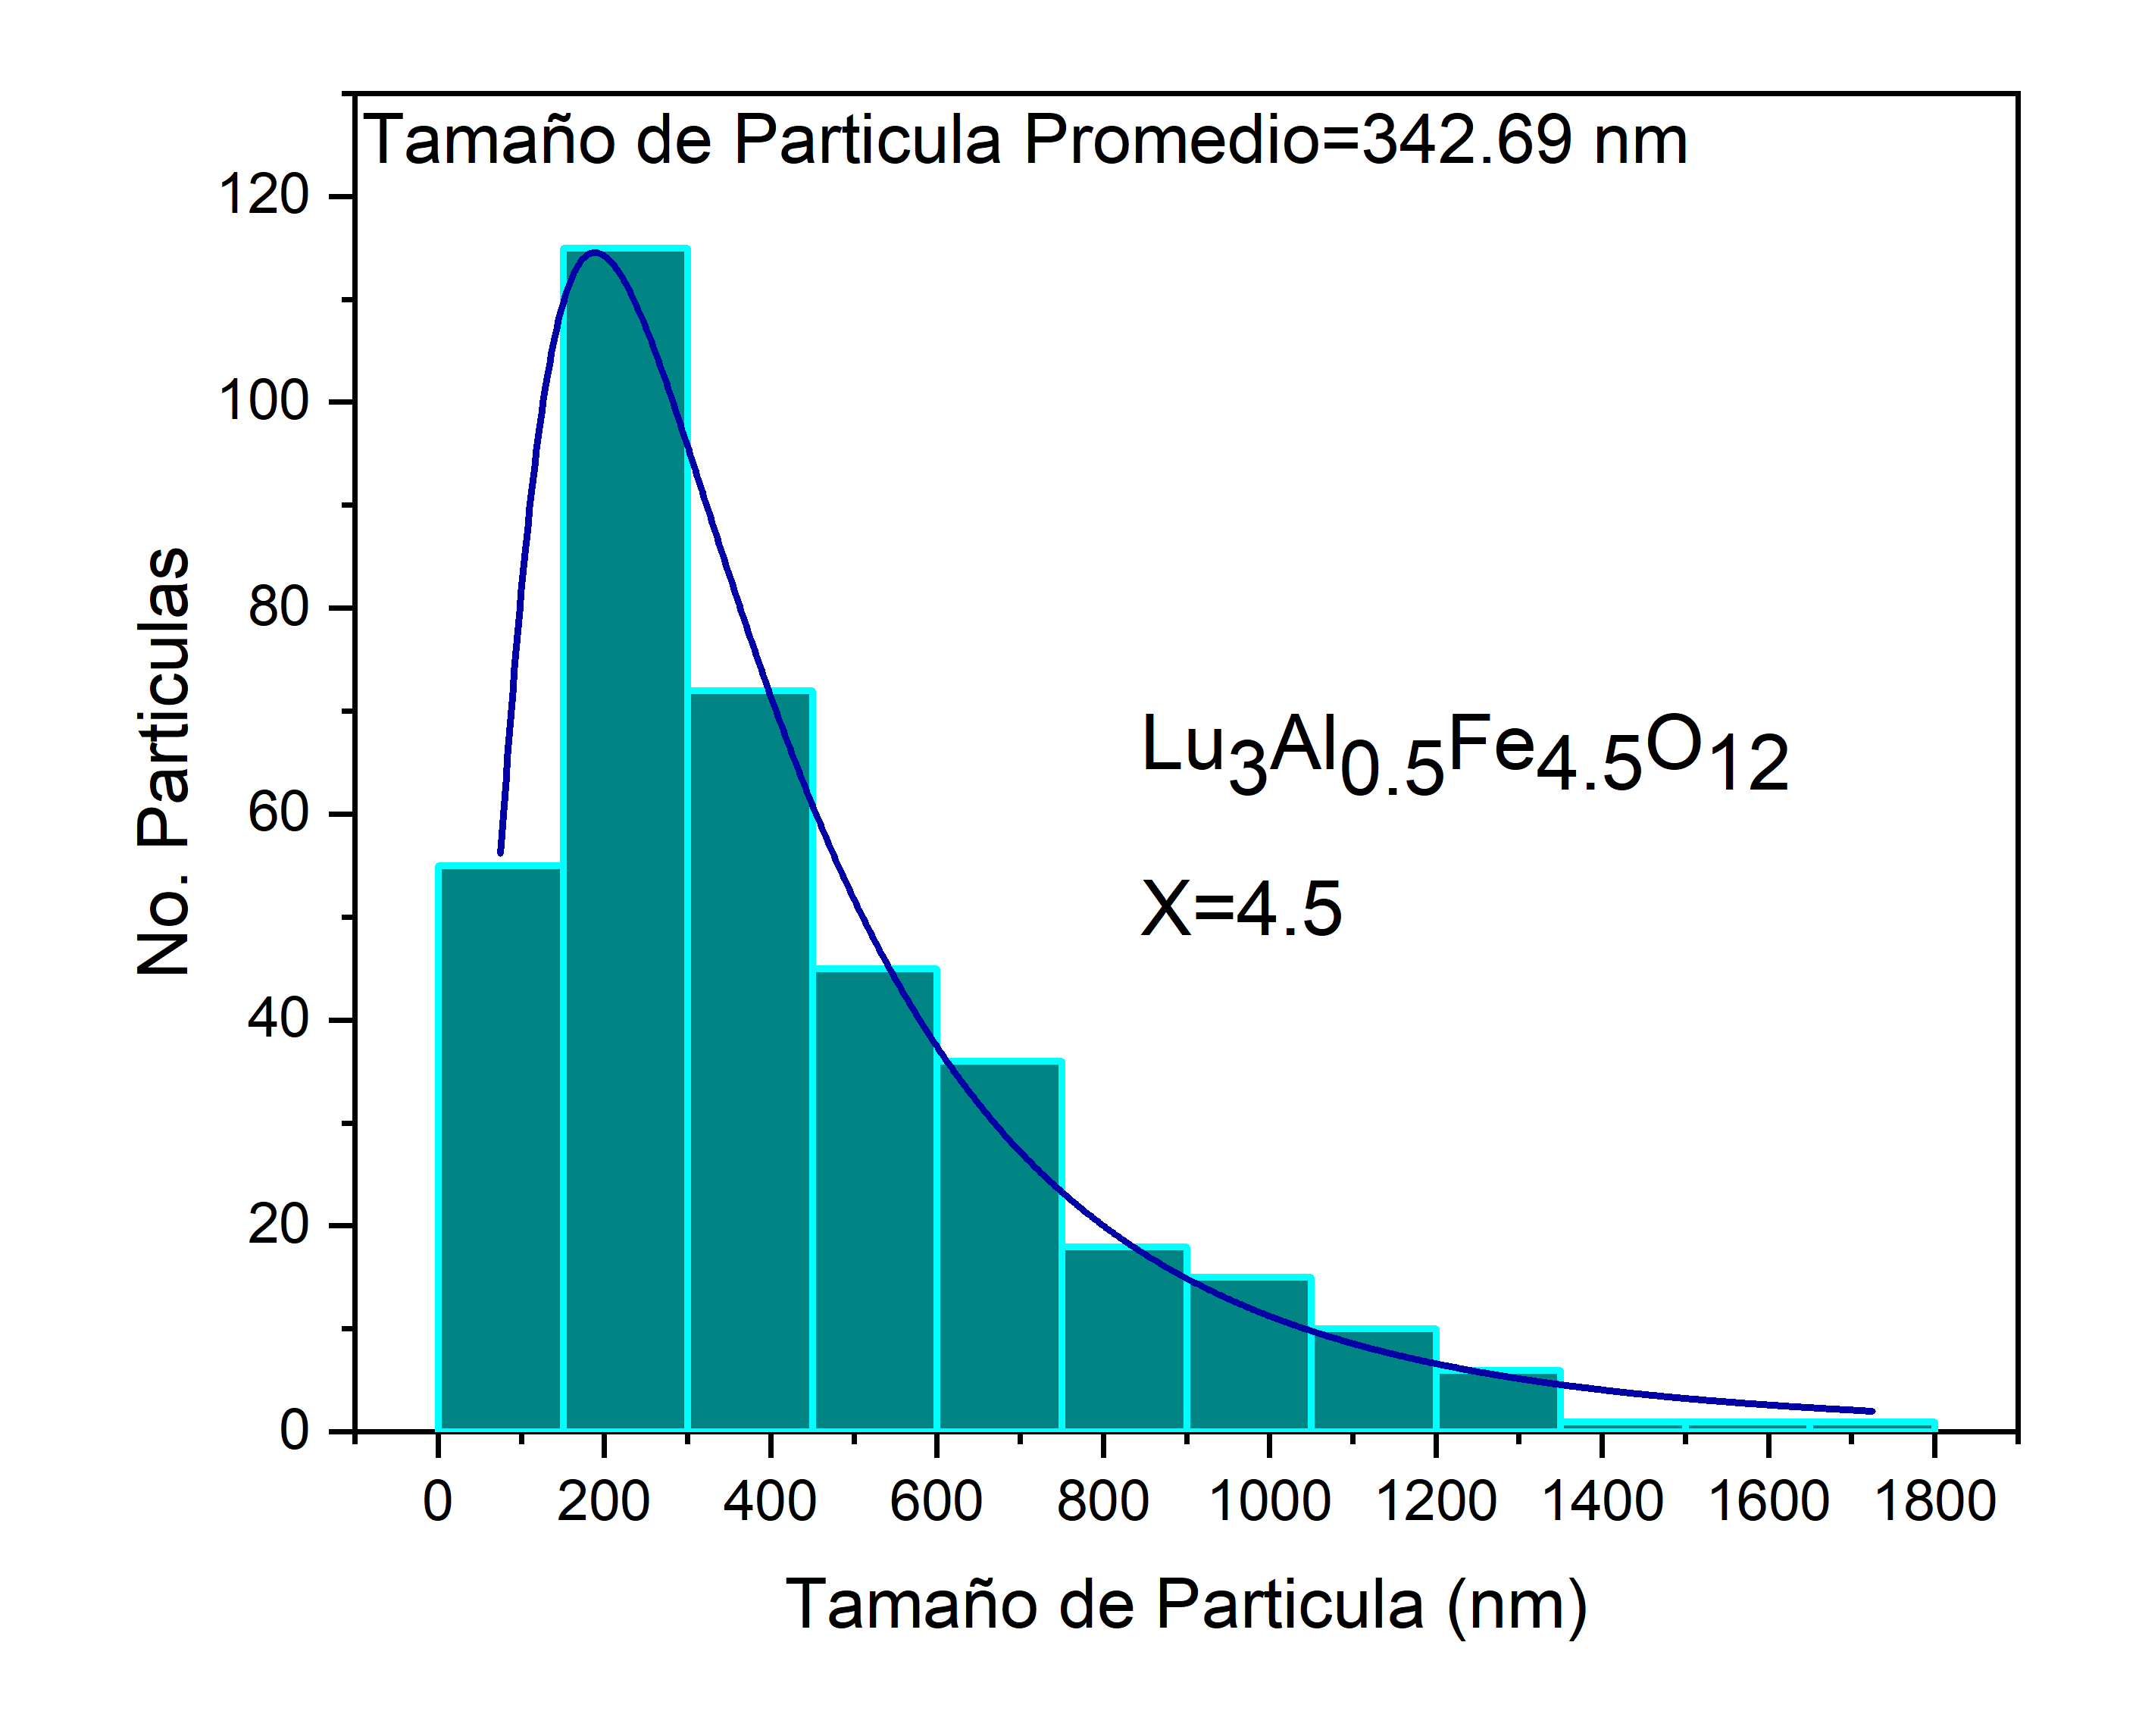
\includegraphics[width=\textwidth]{Kap5/TamG9.png}%
		\caption{Distribución del tamaño de partícula para \ce{Lu_{3.0}Al_{0.5}Fe_{4.5}O12} medida mediante ImageJ}\label{fig:tamG9}
	\end{figure}

	\chapter{EDX}\label{edx}

	\begin{figure}[h]
		\centering%

		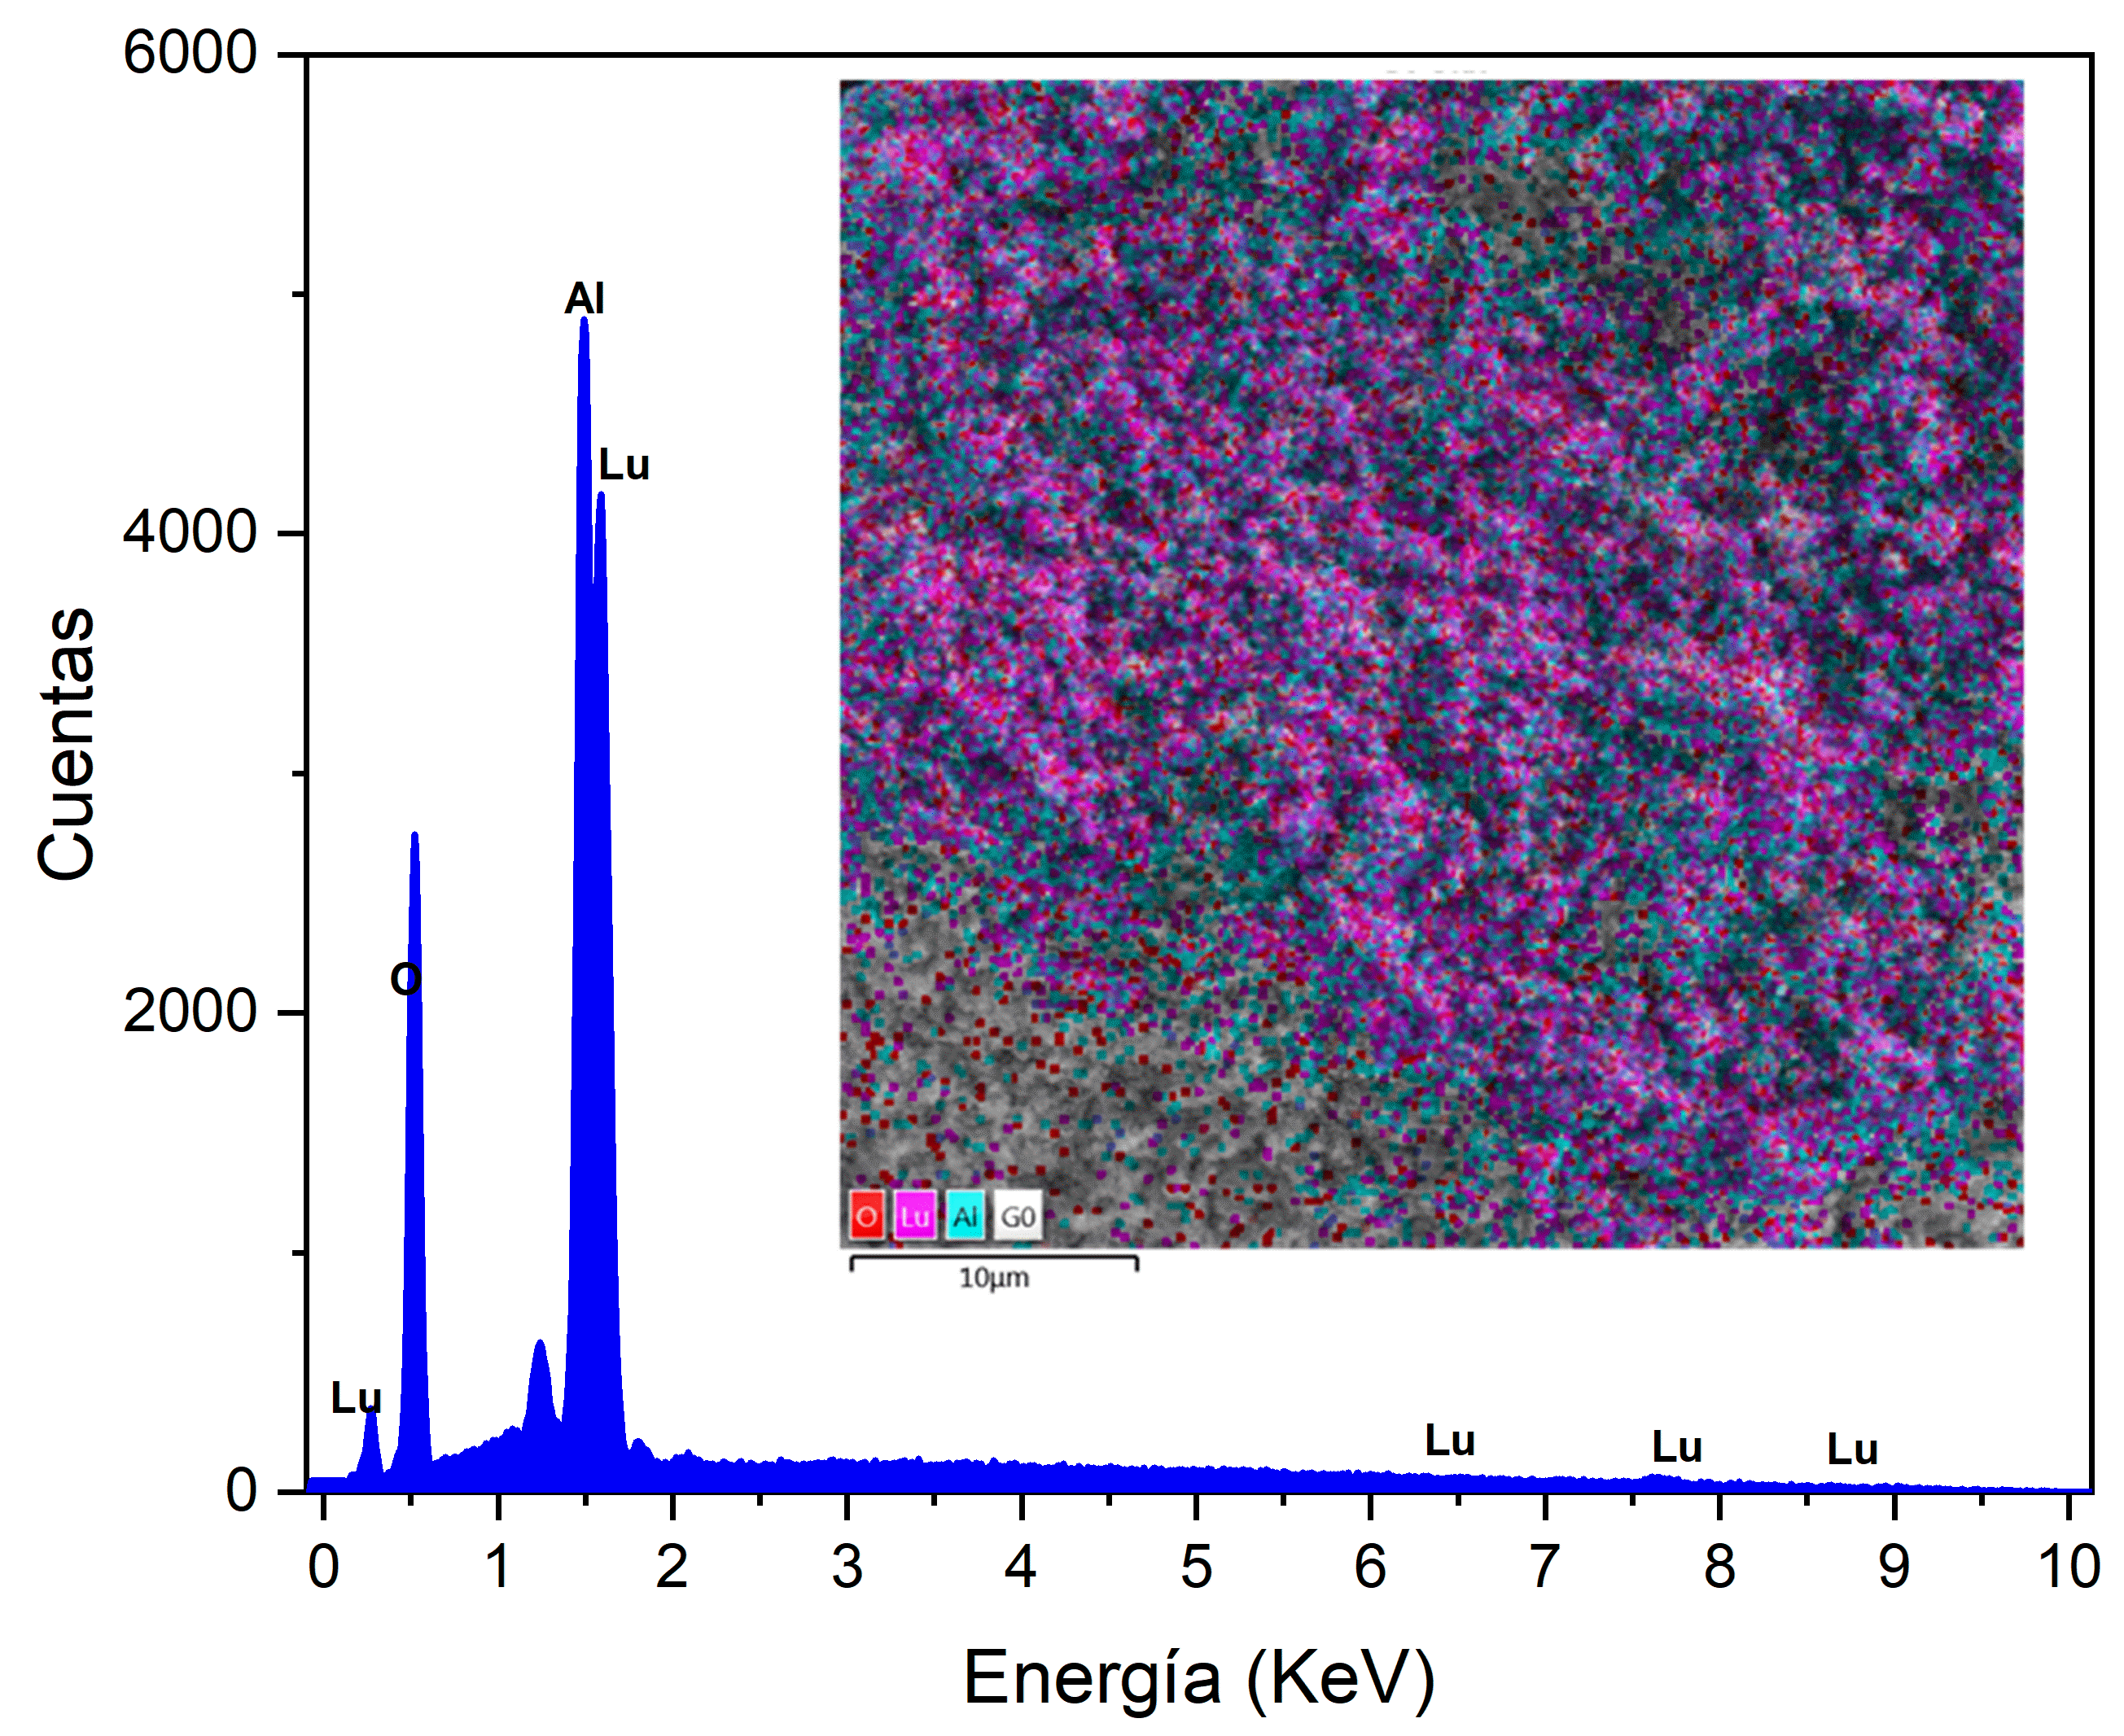
\includegraphics[width=\textwidth]{Anexos/EDXG0.png}%
		\caption{EDX de \ce{Lu_{3.0}Al_{5.0}O12}}\label{fig:edxg0}
	\end{figure}

	\begin{figure}[h]
		\centering%

		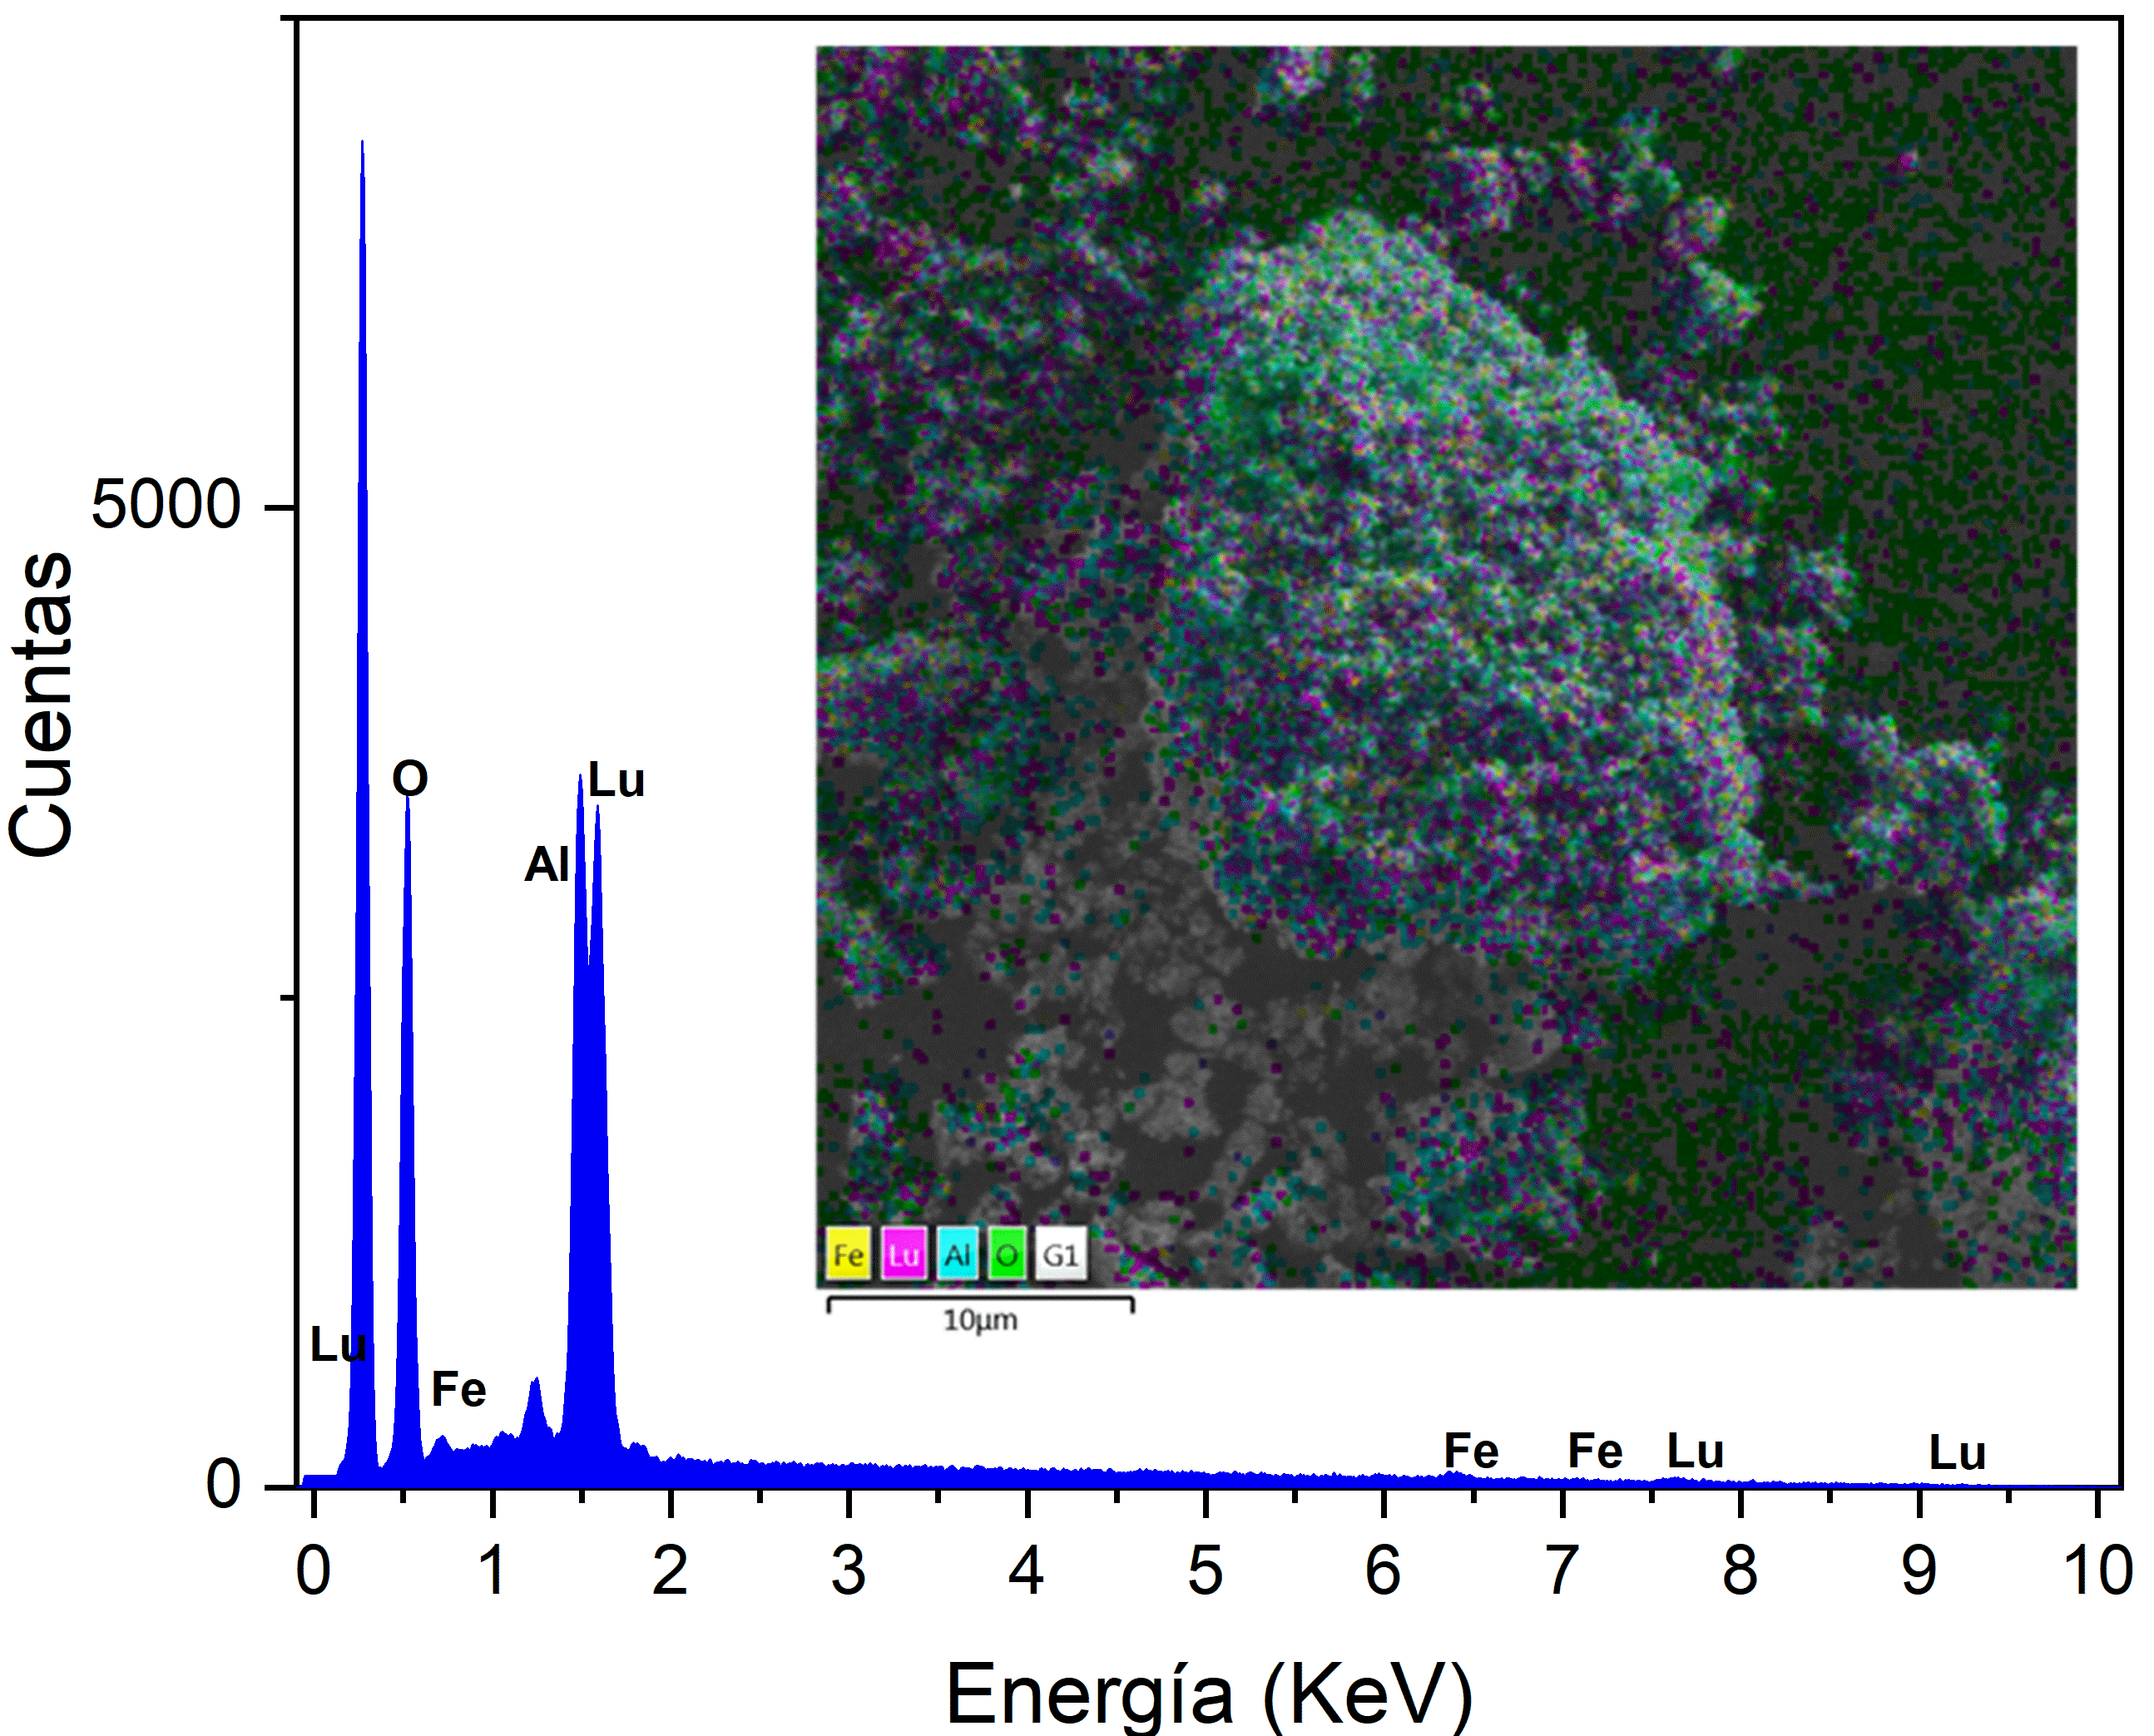
\includegraphics[width=\textwidth]{Anexos/EDXG1.png}%
		\caption{EDX de \ce{Lu_{3.0}Al_{4.5}Fe_{0.5}O12}}\label{fig:edxg1}
	\end{figure}

	\begin{figure}[h]
		\centering%

		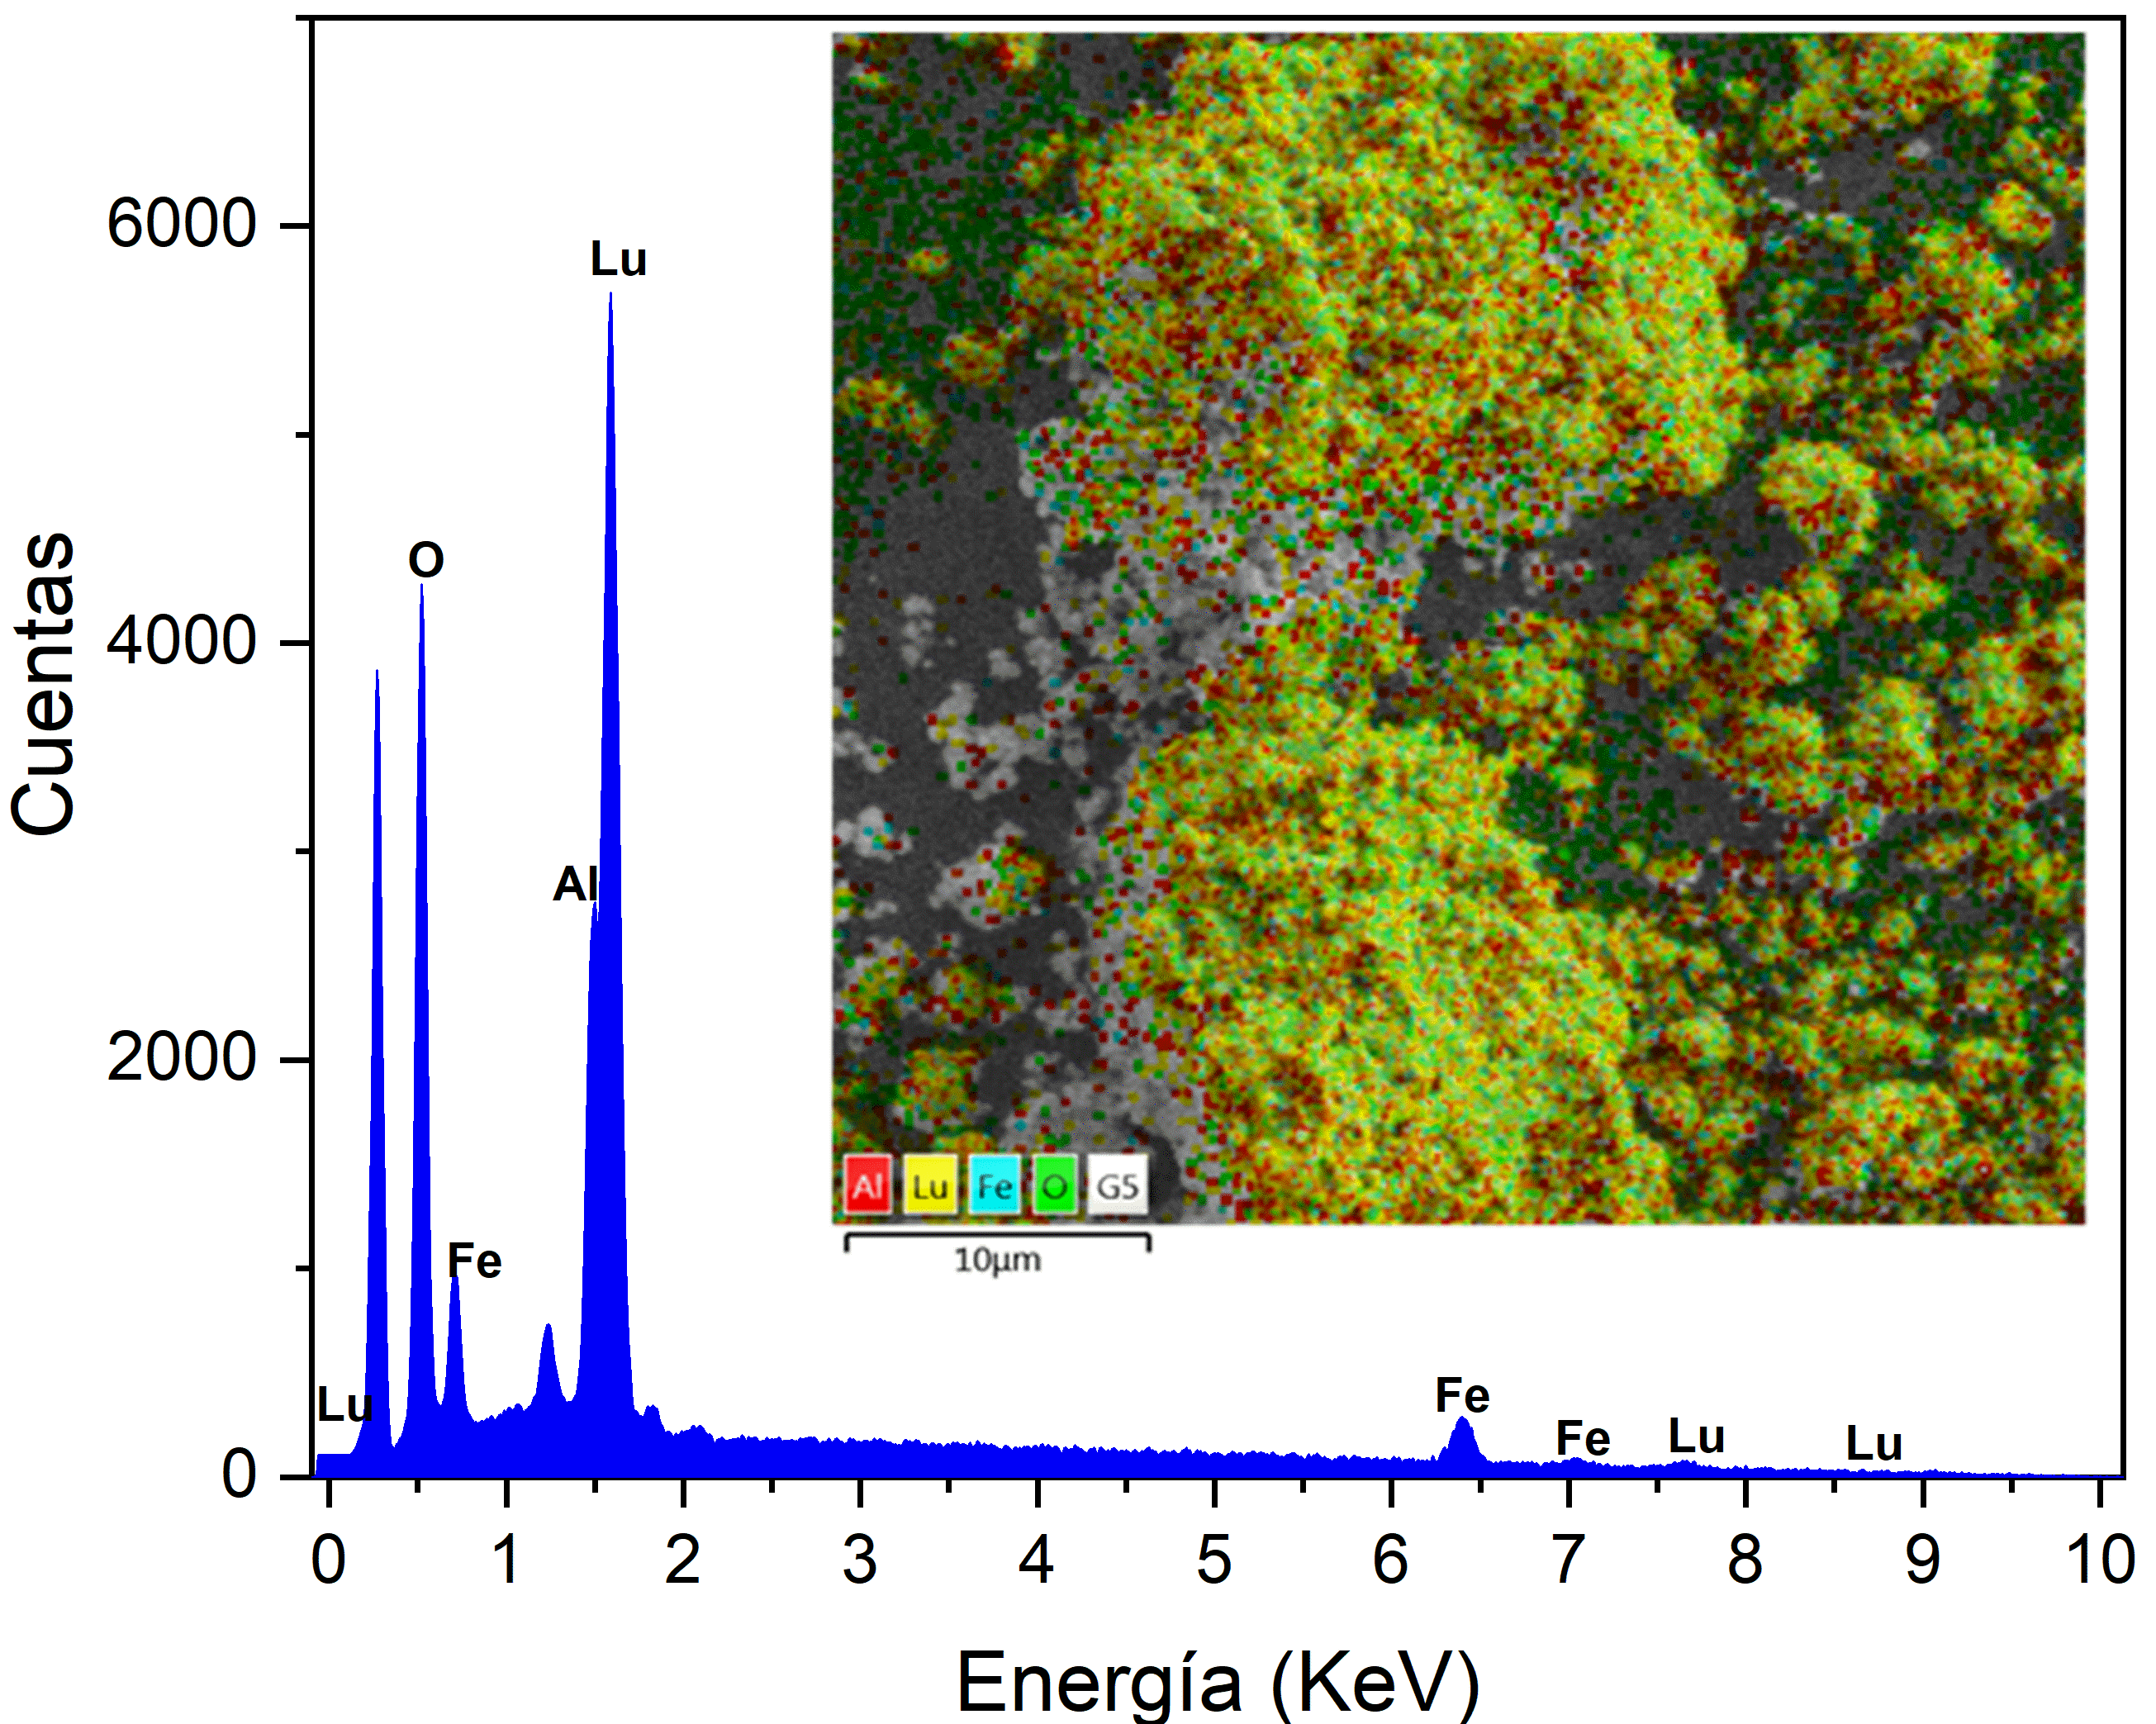
\includegraphics[width=\textwidth]{Anexos/EDXG5.png}%
		\caption{EDX de \ce{Lu_{3.0}Al_{2.5}Fe_{2.5}O12}}\label{fig:edxg5}
	\end{figure}

	\begin{figure}[h]
		\centering%

		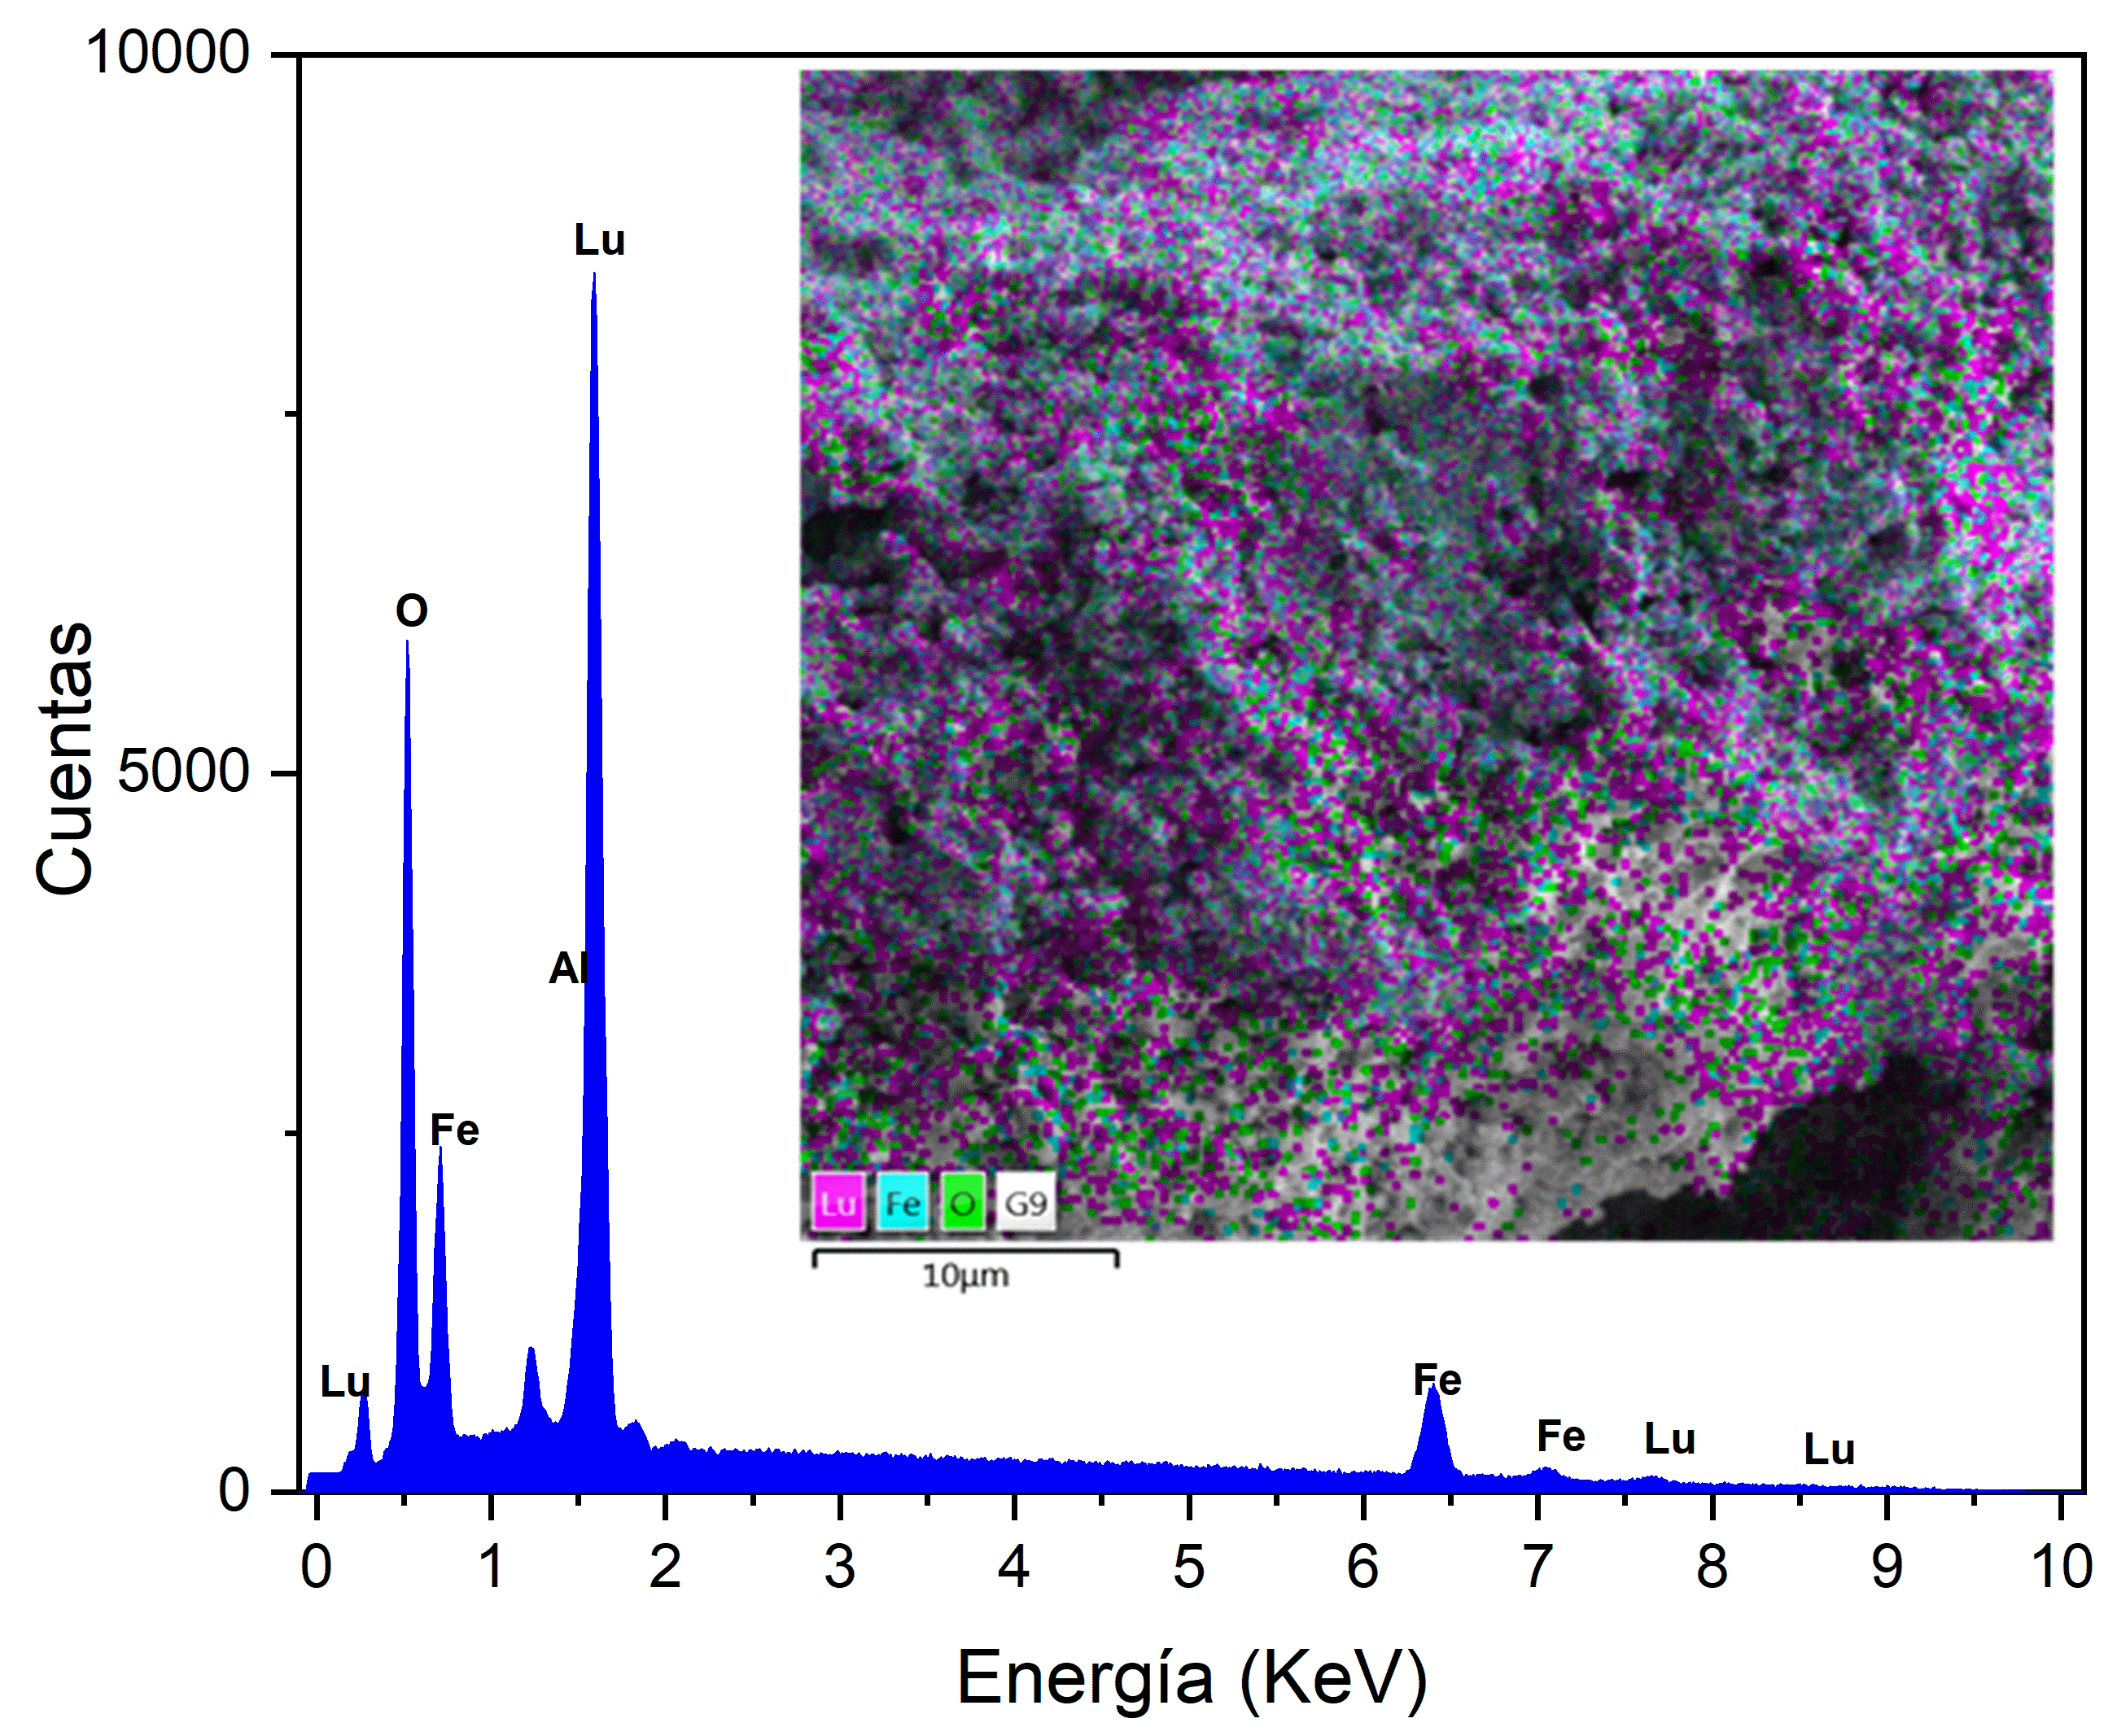
\includegraphics[width=\textwidth]{Anexos/EDXG9.png}%
		\caption{EDX de \ce{Lu_{3.0}Al_{0.5}Fe_{4.5}O12}}\label{fig:edxg9}
	\end{figure}


\end{appendix}